\documentclass{article}

% if you need to pass options to natbib, use, e.g.:
%     \PassOptionsToPackage{numbers, compress}{natbib}
% before loading neurips_2026

% The authors should use one of these tracks.
% Before accepting by the NeurIPS conference, select one of the options below.
% 0. "default" for submission
\PassOptionsToPackage{table}{xcolor}
\usepackage{neurips_2026}
% the "default" option is equal to the "main" option, which is used for the Main Track with double-blind reviewing.
% 1. "main" option is used for the Main Track
%  \usepackage[main]{neurips_2026}
% 2. "position" option is used for the Position Paper Track
%  \usepackage[position]{neurips_2026}
% 3. "eandd" option is used for the Evaluations & Datasets Track
 % \usepackage[eandd]{neurips_2026}
 % if you want to opt-in for a de-anomymized submission (not recommended, but OK):
 %\usepackage[eandd, nonanonymous]{neurips_2026}
% 4. "creativeai" option is used for the Creative AI Track
%  \usepackage[creativeai]{neurips_2026}
% 5. "sglblindworkshop" option is used for the Workshop with single-blind reviewing
 % \usepackage[sglblindworkshop]{neurips_2026}
% 6. "dblblindworkshop" option is used for the Workshop with double-blind reviewing
%  \usepackage[dblblindworkshop]{neurips_2026}

% After being accepted, the authors should add "final" behind the track to compile a camera-ready version.
% 1. Main Track
 % \usepackage[main, final]{neurips_2026}
% 2. Position Paper Track
%  \usepackage[position, final]{neurips_2026}
% 3. Evaluations & Datasets Track
 % \usepackage[eandd, final]{neurips_2026}
% 4. Creative AI Track
%  \usepackage[creativeai, final]{neurips_2026}
% 5. Workshop with single-blind reviewing
%  \usepackage[sglblindworkshop, final]{neurips_2026}
% 6. Workshop with double-blind reviewing
%  \usepackage[dblblindworkshop, final]{neurips_2026}
% Note. For the workshop paper template, both \title{} and \workshoptitle{} are required, with the former indicating the paper title shown in the title and the latter indicating the workshop title displayed in the footnote.
% For workshops (5., 6.), the authors should add the name of the workshop, "\workshoptitle" command is used to set the workshop title.
% \workshoptitle{WORKSHOP TITLE}

% "preprint" option is used for arXiv or other preprint submissions
 % \usepackage[preprint]{neurips_2026}

% to avoid loading the natbib package, add option nonatbib:
% \usepackage[nonatbib]{neurips_2026}

\usepackage[utf8]{inputenc} % allow utf-8 input
\usepackage[T1]{fontenc}    % use 8-bit T1 fonts
\usepackage{hyperref}       % hyperlinks
\usepackage{url}            % simple URL typesetting
\usepackage{booktabs}       % professional-quality tables
\usepackage{amsfonts}       % blackboard math symbols
\usepackage{nicefrac}       % compact symbols for 1/2, etc.
\usepackage{microtype}      % microtypography
% xcolor loaded via \PassOptionsToPackage above
\usepackage{microtype}
\usepackage{hyperref}
\usepackage{url}
\usepackage[most]{tcolorbox}
\usepackage{multirow}
\usepackage{graphicx}
\usepackage{booktabs}
\usepackage[table]{xcolor}
\usepackage{amsmath}
\usepackage{pifont}
\usepackage{algorithm}
\usepackage{algpseudocode}
\usepackage{float}
\usepackage{amsfonts}
\usepackage{tabularx}
\usepackage{multicol}
\usepackage{caption}
\usepackage{subcaption}
\usepackage{refcount}
\usepackage{makecell}
\usepackage{newfloat}
\usepackage{listings}
\usepackage{adjustbox}
\usepackage{wrapfig}
\usepackage{amssymb}
\usepackage{caption}
\usepackage{amsthm}
\usepackage{enumitem}
\theoremstyle{remark}
\usepackage{array}

\newtheorem{prop}{Proposition}
\newtheorem*{remark}{Remark}

% NOTE: including geometry package
% The geometery package modifies some page properties when used. This can dramatically change the page margins, leading to severe template violation, and potential desk rejection. If the package is required, it can be used with the "pass" flag to skip the default page modifications, as in the following line:
% \usepackage[pass]{geometry}

\usepackage{lineno}

\definecolor{darkblue}{rgb}{0, 0, 0.5}
\hypersetup{colorlinks=true, citecolor=darkblue, linkcolor=darkblue, urlcolor=darkblue}


\title{Efficient Best-Of-$N$ with Radial Consensus Score}

% Authors must not appear in the submitted version. This should be be taken care of automatically as long as you are using the "submission" option for the colm2026_conference package. But it's on the authors to verify. Non-anonymous submissions will be rejected without review.

\author{Antiquus S.~Hippocampus, Natalia Cerebro \& Amelie P. Amygdale \thanks{ Use footnote for providing further information
about author (webpage, alternative address)---\emph{not} for acknowledging
funding agencies.  Funding acknowledgements go at the end of the paper.} \\
Department of Computer Science\\
Cranberry-Lemon University\\
Pittsburgh, PA 15213, USA \\
\texttt{\{hippo,brain,jen\}@cs.cranberry-lemon.edu} \\
\And
Ji Q. Ren \& Yevgeny LeNet \\
Department of Computational Neuroscience \\
University of the Witwatersrand \\
Joburg, South Africa \\
\texttt{\{robot,net\}@wits.ac.za} \\
\AND
Coauthor \\
Affiliation \\
Address \\
\texttt{email}
}

% The \author macro works with any number of authors. There are two commands
% used to separate the names and addresses of multiple authors: \And and \AND.
%
% Using \And between authors leaves it to \LaTeX{} to determine where to break
% the lines. Using \AND forces a linebreak at that point. So, if \LaTeX{}
% puts 3 of 4 authors names on the first line, and the last on the second
% line, try using \AND instead of \And before the third author name.

\newcommand{\fix}{\marginpar{FIX}}
\newcommand{\new}{\marginpar{NEW}}

\begin{document}

\maketitle

\begin{abstract}

Solving complex problems with large language models (LLMs) often requires selecting the best answer from multiple candidate responses (best-of-$N$), yet identifying the most reliable one remains challenging, particularly when correctness does not align with majority agreement.
Existing approaches based on voting or probability scoring rely on surface-level signals (e.g., frequency or token-level likelihood), often missing high-quality rare answers and ignoring the geometric structure of candidate representations, where correctness may emerge as semantic consistency rather than surface agreement.
To address these limitations, we introduce \textbf{Radial Consensus Score (RCS)}, a simple, efficient, and training-free method for best-of-$N$ selection. 
RCS models semantic consensus by computing a weighted Fréchet mean (semantic center)of answer embeddings and ranking candidates by their radial distance to this center. Importantly, RCS offers a flexible framework that supports multiple weighting schemes, enabling the integration of agreement signals and model confidence, where the position of center adapts accordingly.
% RCS further supports flexible weighting schemes to integrate agreement signals and model confidence, with the center adapting accordingly---for example, uniform averaging treats all candidates equally, while frequency or probability weighting shifts it toward more consistent or higher-confidence responses.
% RCS further provides a flexible framework that supports multiple weighting schemes, enabling the integration of agreement signals and model confidence. 
% The position of this center adapts to different consensus signals through the choice of weighting scheme: uniform averaging treats all candidates equally, while frequency or probability weighting shifts the center toward more consistent or higher-confidence responses.
% RCS provides a general framework that supports multiple weighting schemes, enabling flexible integration of agreement signals and model confidence while remaining fully applicable in black-box settings.
% In practice, the consensus center can be instantiated via standard embedding space averaging or other weighted aggregation methods, depending on the available signals.
Extensive experiments across various benchmarks covering short-form QA and long-form reasoning tasks, and five open-weight models, demonstrate that our metrics consistently outperform strong baselines with advantages growing as $N$ increases.
Moreover, RCS also serves as an effective drop-in replacement for majority voting in multi-agent debate and exhibits strong robustness in black-box scenarios.
These results highlight geometric consensus as an applicable and scalable principle for reliable answer selection beyond majority voting.
\end{abstract}

\section{Introduction}

Large language models (LLMs) have achieved remarkable progress across diverse tasks, yet they remain prone to generating inconsistent or incorrect outputs, particularly in open-ended or reasoning-intensive scenarios~\citep{wang2022self, huang2025survey}. A common strategy to improve reliability is best-of-$N$ sampling: generate multiple candidate responses from the same prompt and select the highest-quality one according to a scoring mechanism~\citep{cobbe2021training, wang-etal-2024-math, kang2025scalable}. In this framework, performance critically depends not only on the diversity of sampled candidates but, more importantly, on the effectiveness of the selection criterion.

Existing selection methods can be broadly categorized into two groups. The first relies on \emph{external evaluators}, such as reward models or verifiers, to score each candidate~\citep{cobbe2021training, lightman2023let}. While effective, these approaches introduce additional computational overhead and require extra supervision. The second group uses \emph{intrinsic signals} derived from the sampled responses themselves. The dominant paradigm in this category is self-consistency via majority voting, which assumes that correct answers appear most frequently among samples~\citep{wang2022self}. This works well when the answer space is discrete, but it struggles in settings with semantic ambiguity or when high-quality minority answers are underrepresented despite being semantically close to the consensus~\citep{chen2023universal, kang2025scalable}.
Recent work has also proposed ranked or reasoning-aware extensions of self-consistency, such as Borda-style voting, along with theoretical analyses connecting Best-of-$N$ to mode estimation and KL-constrained optimization~\citep{gui2024bonbon, wang2025ranked, wan2025reasoning, cordero2025certified}. Parallel efforts explore weighted aggregation and hybrid selection strategies, such as correlation-aware multi-agent weighting and Best-of-Majority, to improve reliability and scaling behavior~\citep{ai2025beyond, di2025best}.

However, these approaches often rely on additional sampling or surface-form agreement, limiting their practicality in real-world settings, especially when efficient, black-box-compatible, and training-free selection is required. 
As illustrated in Figure~\ref{fig:overview}, these limitations arise from a mismatch between surface-level signals and the underlying semantic structure of candidate answers.
This raises a central question: \emph{Can we develop an efficient and training-free selection framework that operates directly in answer space, enabling robust per-sample ranking without relying on external supervision or costly sampling procedures?}
% ============

To tackle this question, we introduce the \textbf{Radial Consensus Score (RCS)}, a principled geometric approach for efficient best-of-N selection. Our key insight is to model semantic consensus explicitly via a weighted Fréchet mean~\citep{fletcher} as the semantic center of answer embeddings and then rank candidates by their radial distance to this center. This formulation naturally incorporates both semantic agreement structure and optional confidence signals (frequency, generation probability, or pairwise cosine similarity) through the choice of weighting distribution $P$.
Different choices of $P$ recover a spectrum of selection strategies, ranging from uniform weighting that treats all candidates equally to frequency-based, probability-based, and cosine-similarity-based schemes that emphasize consensus, model confidence, or mutual agreement. This flexibility allows the framework to adapt to different inference settings while remaining fully training-free and black-box compatible.
The resulting score is computationally lightweight, model-agnostic, and directly yields a ranking of individual candidates without requiring clustering or external verifiers.
We evaluate RCS on seven established benchmarks spanning short-form QA (SciQ, GPQA), mathematical reasoning (Arithmetics, GSM8K), and long-form multiple-choice tasks (MMLU Formal Logic, MMLU-Pro, BigBenchHard), using five diverse open-weight models. RCS variants consistently outperform strong baselines---including Semantic Consensus Weighting (SCW)---by 2--7\% in selection accuracy, with gains becoming more pronounced as the sampling budget increases. Additional analyses confirm their efficiency and robustness in black-box settings and multi-agent debate scenarios.
Our contributions are threefold:
\textbf{First}, we introduce Radial Consensus Score (RCS), a geometric consensus framework for best-of-$N$ selection that bridges probability-based and surface-form methods, and prove, under a Gaussian generative model, that it outperforms voting in both infinite- and finite-sample regimes under sufficient semantic-separation conditions.
% \textbf{First}, we introduce Radial Consensus Score (RCS), a geometric consensus framework for best-of-$N$ selection that bridges probability-based and surface-form methods, grounded in a closed-form formulation via the Fréchet mean and its discrete medoid counterpart. 
\textbf{Second}, comprehensive experiments across diverse tasks and models demonstrate that RCS consistently outperforms strong baselines, with gains increasing as the sampling budget grows, highlighting favorable scaling behavior.
\textbf{Third}, ablation studies further confirm the effectiveness and applicability of RCS, showing its robustness in multi-agent debate and fully black-box settings, along with strong practical efficiency, underscoring its impact as a scalable aggregation method for LLM inference.


\begin{figure*}[t]
    \centering
    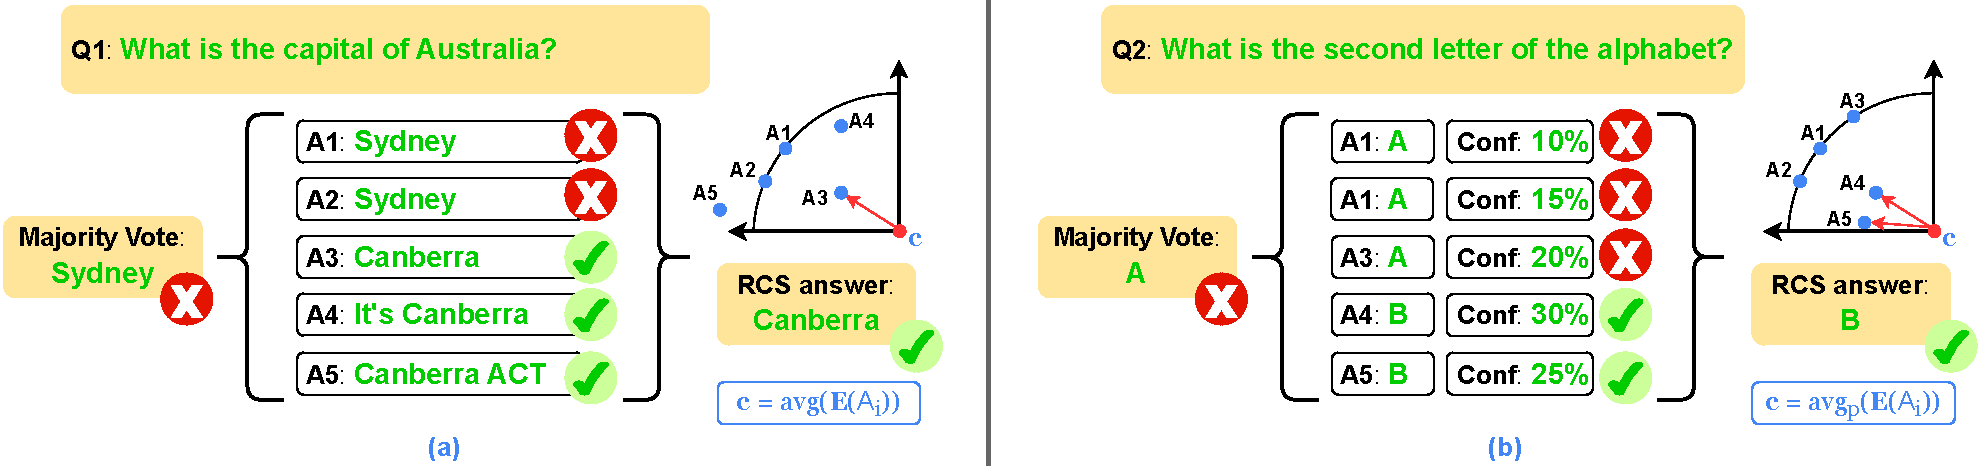
\includegraphics[width=\textwidth]{plots/RDS_overview.pdf}
    \caption{
        RCS overview and representative failure modes of majority voting.
        (a) Majority voting ignores semantically similar answers by treating surface forms independently.
        (b) It also fails to select high-confidence but minority answers.
        RCS addresses both issues by mapping answers into an embedding space via Encoder $\mathbf{E}$ and estimating a centroid $\mathbf{c}$, either \textit{uniformly} or \textit{probability-weighted} over answer embeddings. Additional qualitative examples are provided in Section~\ref{sec:qualitative}.}
    \label{fig:overview}
\end{figure*}

\section{Related Work}

\paragraph{Best-Of-$N$ Metrics.}
Self-consistency, in its most common form, performs majority voting over $N$ sampled candidates~\citep{wang2022self}. 
Extensions such as universal and fine-grained self-consistency improve robustness but often incur extra LLM calls for evaluation or refinement~\citep{chen2023universal,wang2024integrate}. 
Alternatively, self-certainty directly leverages the model's output probability distribution to estimate response quality without external reward models, showing strong scaling with $N$~\citep{kang2025scalable}.
Beyond voting-based strategies, recent advances include ranked and reasoning-aware aggregation, e.g. Borda-style voting~\citep{wang2025ranked, wan2025reasoning}. 
From a theoretical perspective, Best-of-$N$ has been analyzed under sampling and alignment objectives, linking it to mode estimation and KL-constrained optimization~\citep{gui2024bonbon, cordero2025certified}.
Several concurrent works employ embedding-space geometry for answer selection, from dispersion-based uncertainty estimation~\citep{nguyen2025distance} to trajectory-level clustering.
\textit{Centroid-based MBR}~\citep{deguchi2024centroid} selects the hypothesis nearest to the unweighted centroid to minimize expected error, incurring higher computational costs.
A further group of methods embeds full reasoning trajectories, sharing a representation-collapse problem: \textit{Latent Self-Consistency}~\citep{chen2024latent} and \textit{ModeX}~\citep{choi2026modex} apply latent-space clustering at higher computational cost; 
\textit{Semantic Consensus Weighting}~\citep{jain2023sc} computes pairwise cosine similarities and selects the highest-scoring trajectory group via a discrete aggregation step, additionally inheriting the minority-answer blindness of majority voting.
RCS unifies these directions in a single closed-form weighted Fr\'echet mean at the \emph{final-answer} level, avoiding embedding-collapse or discrete grouping step while remaining efficient.

\paragraph{Uncertainty Estimation For LLMs.}
Uncertainty estimation for LLMs is typically categorized into probability-based and semantic families.
(1) \textit{Probability-based methods} rely on token-level likelihoods such as negative log-likelihood or predictive entropy~\citep{guerreiro2022looking,manakul2023selfcheckgpt}. Recent improvements like PRO approximate entropy efficiently from the top-$K$ probabilities with adaptive noise filtering~\citep{nguyen2025probabilities}. These methods perform well on open-weight models but are inapplicable to black-box APIs and often require calibration.
(2) \textit{Semantic entropy-based methods} shift the focus to meaning by clustering responses in embedding space and computing entropy over cluster distributions or densities~\citep{kuhn2023semantic,farquhar2024detecting,lin2023generating, nikitin2024kernel, qiu2024semantic}. Extensions include evidential semantic entropy for handling uncertainty~\citep{kunitomo-jacquin-etal-2026-evidential} and geometric dispersion measures such as semantic volume~\citep{li2026semantic}.
Parallel work explores token-level uncertainty through low-rank weight perturbation~\citep{zhang2025tokur} and confidence-aware filtering of reasoning traces~\citep{fu2025deep}.
While these methods effectively quantify uncertainty at the set level, they largely ignore the LLM's native probability signals, are sensitive to clustering quality or computationally expensive, and require additional post-processing for individual candidate scoring.
Our method bridges probabilistic and semantic perspectives, enabling efficient per-sample ranking.

% ================
\section{Methodology}\label{sec:method}

% We model semantic consensus via a weighted Fréchet mean of answer embeddings, where the weighting distribution can optionally incorporate additional signals such as frequency or model confidence. The resulting semantic center is then used to rank candidates according to their distances to it. We provide the detailed pseudo-code for our method in Appendix Algorithm~\ref{alg:rds}.

\subsection{Problem Statement}\label{sec:problem}

Given a prompt $x$, we sample $N$ independent generations $\{y_1, \dots, y_N\}$ from a language model using multinomial decoding. Each generation is mapped to a final answer $\{a_i\}_{i=1}^N$, optionally associated with generation likelihoods $\{p(y_i | x)\}_{i=1}^N$.
Our goal is to identify the most reliable answer among the candidates. Formally, we consider the problem:
\begin{align}
    a^* = \arg\max_{a_i} \; Q(a_i|x),
\end{align}
where $Q(a_i|x)$ denote an unknown quality function reflecting the correctness or reliability of an answer, which must be estimated from a set of sampled generations. 
% Existing approaches, such as self-consistency~\citep{wang2022self}, approximate $Q(a_i \mid x)$ using answer frequency, implicitly assuming that correct answers appear more often. However, such discrete aggregation ignores semantic relationships between answers and treats all disagreements equally, motivating the need for a more expressive estimator of answer quality.

\subsection{Answer Selection via Geometric Consensus}~\label{sec:center}

To approximate the latent quality function $Q(a_i|x)$, we propose to model agreement among answers in a continuous semantic space. Formally, we embed each final answer into a vector space:
\begin{align}
    \mathbf{u}_i = \mathbf{E}(a_i),
\end{align}
where $\mathbf{E}$ is a sentence embedding model. 
Intuitively, in the context of best-of-$N$, sampled answers form a distribution of semantic interpretations of the same query, and a representative solution should reflect their overall agreement. The Fréchet mean~\citep{fletcher} defines such a centroid as the point that minimizes the expected squared distance to all candidate embeddings in the semantic space. Given embeddings $\{\mathbf{u}_i\}_{i=1}^N \subset \mathbb{R}^d$ with a probability distribution $P{=}\{p_i\}_{i=1}^N$, the semantic center is defined as the Fréchet mean under squared Euclidean loss:
\begin{align}
    \mathbf{c}(P) = \arg\min_{\mathbf{z}} \sum_{i=1}^N p_i \|\mathbf{u}_i - \mathbf{z}\|_2^2,
        \label{eq:center}
\end{align}
This admits the closed-form solution:
\begin{align}
    \mathbf{c}(P) = \sum_{i=1}^N p_i \mathbf{u}_i,
\end{align}
(see Appendix~\ref{app:proof_center} for details).

We adopt the squared Euclidean loss for its simple closed-form solution. When the center is restricted to the discrete set $\{\mathbf{u}_i\}_{i=1}^N$, the problem reduces to selecting a representative sample:
\begin{align}
\mathbf{c}_{\text{medoid}}(P)
= \arg\min_{\mathbf{u}_j} \sum_{i=1}^N p_i \|\mathbf{u}_i - \mathbf{u}_j\|_2^2,
\end{align}
which corresponds to a weighted medoid. This can be viewed as a discrete counterpart of the Fréchet mean, where the solution is constrained to be one of the observed samples.

Different choices of $P$ (Table~\ref{tab:rds_variants}) induce different notions of semantic consensus. In particular, the uniform distribution recovers the standard unweighted center, while frequency-based or likelihood-based distributions incorporate empirical or model-derived reliability signals.
Conceptually, $\mathbf{c}(P)$ represents a consensus embedding of the generated answers, with semantically similar answers pulling the center toward their shared meaning and divergent or noisy samples contributing proportionally to their weights in $P$ (see Figure~\ref{fig:overview}).
% Intuitively, $\mathbf{c}(P)$ represents a consensus embedding of the generated answers. Semantically similar answers pull the center toward their shared meaning, while divergent or noisy samples exert influence proportional to their weights in $P$ (see Figure~\ref{fig:overview}).

\subsection{Ranking via Radial Consensus Score}\label{sec:main-rcs}

Given a semantic center $\mathbf{c}(P)$, we define a ranking function based on the radial dispersion of each candidate embedding relative to this center.
For each candidate embedding $\mathbf{u}_i$, its \textbf{Radial Consensus Score} (RCS) is defined as:
\begin{align}
    \mathrm{RCS}_i(P) = \|\mathbf{u}_i - \mathbf{c}(P)\|_2.
\end{align}
% where $\mathbf{c}(P)$ is defined in Section~\ref{sec:center}.
RCS measures how semantically aligned each candidate is with the global consensus induced by the distribution $P$: smaller values indicate stronger agreement with the collective semantic structure, while larger values suggest divergence or potential noise. 
We adopt the $\ell_2$ norm for its simplicity and consistency with the center formulation (Equation~\ref{eq:center}), as the choice of norm does not materially affect the relative ranking of candidates in practice.

\begin{table*}[t]
\centering
\caption{Different instantiations of the distribution $P$ in RCS, where $f_i$ and $\Pr(y_i|\mathbf{x})$ denote the empirical frequency and model probability of candidate $y_i$, respectively. For the frequency-weighted variant, the index $i$ runs over the set of \emph{unique} answers, so that $\sum_j f_j = N$. For the cosine-similarity-weighted variant, $\cos(\mathbf{u}_i,\mathbf{u}_j)$ denotes the cosine similarity between $L_2$-normalized embeddings.}
\label{tab:rds_variants}
\begin{tabular}{l l l}
\toprule
\textbf{Variant} & \textbf{Distribution $P$} & \textbf{Note} \\
\midrule
Uniform & $p_i = \frac{1}{N}$ & Black-box\\
Frequency-weighted & $p_i = \frac{f_i}{\sum_j f_j}$ & Black-box\\
Probability-weighted & $p_i \propto \Pr(y_i|\mathbf{x})$ & White-box (calibrated)\\
Cosine-weighted & $p_i \propto \frac{1}{N}\sum_{j=1}^N \cos(\mathbf{u}_i,\mathbf{u}_j)$ & Black-box\\
\bottomrule
\end{tabular}
\end{table*}

The final prediction is selected as the candidate with minimum radial dispersion to the estimated consensus:
\begin{align}
    a^*(P) = \arg\min_{a_i} \mathrm{RCS}_i(P).
\end{align}

In discrete settings, the above objective admits an equivalent \textbf{weighted medoid} formulation:
\begin{align}
    a^*(P) = \arg\min_{a_i} \sum_{j} P(a_j)\,\|\mathbf{u}_i - \mathbf{u}_j\|_2^2.
\end{align}
This selects the candidate whose embedding minimizes the expected \emph{squared} distance to others under $P$, consistent with the squared-Euclidean Fréchet mean objective (Equation~\ref{eq:center}). When $P$ is uniform, this reduces to the standard medoid.


\paragraph{Theoretical Analysis.}
To formally characterize the behavior of RCS, we model the answer embeddings as draws from a Gaussian noise distribution centered at the true semantic center--that is, $\mathbf{u}_i = \mathbf{c}^* + \boldsymbol{\varepsilon}_i$ with $\boldsymbol{\varepsilon}_i \sim \mathcal{N}(\mathbf{0}, \sigma^2\mathbf{I})$. 
Under this generative assumption, we establish two propositions showing that RCS is strictly superior to majority voting, formulated as follows. The uniform, frequency, and probability-weighted variants admit direct proofs via the strong law of large numbers; the cosine-similarity-weighted variant satisfies the same asymptotic guarantee under an additional regularity condition (Appendix~\ref{app:proof_prop1}).
% with detailed proofs deferred to Appendix~\ref{app:proof_prop1} and~\ref{app:proof_prop2}.

\begin{prop}[\textbf{Asymptotic Superiority}]
Under the Gaussian generative model, for \emph{any} of the four distributions \(P\) (Table~\ref{tab:rds_variants}), as \(N \to \infty\),
\begin{align}
\mathbf{c}(P) \xrightarrow{a.s.} \mathbf{c}^*,
\end{align}
by the strong law of large numbers. Consequently,
\begin{align}
\mathbb{P}(\text{RCS selects $a^*$}) \to 1, \quad \mathbb{P}(\text{voting selects $a^*$}) \leq \frac{1}{M},
\end{align}
where $a^*$ is the true best answer (corresponding to $\mathbf{c}^*$) and \(M \geq 2\) is the number of distinct semantic clusters (typically \(M \gg 1\) in open-ended generation). Thus RCS is asymptotically strictly superior to majority voting whenever lexical variance (due to paraphrasing) exceeds semantic variance.
% \qed
\end{prop}
\begin{proof}
    See Appendix~\ref{app:proof_prop1}.
\end{proof}
% \qed

\begin{prop}[\textbf{Finite-\(N\) Gap with 2-Cluster Toy Model}]
Consider the following two-cluster setting: (1) Cluster A (true high-quality): \(k \geq N/2\) samples centered at \(\mathbf{c}^* + \boldsymbol{\delta}\), \(\|\boldsymbol{\delta}\|_2\) small; and (2) Cluster B (spurious): \(N-k\) samples centered at \(\mathbf{c}^* + \boldsymbol{\Delta}\), \(\|\boldsymbol{\Delta}\|_2 \gg \|\boldsymbol{\delta}\|_2\).

Under the frequency-weighted distribution, the empirical center \(\mathbf{c}(P)\) is geometrically biased toward Cluster A when \(k \geq N/2\). Approximating each cluster's candidates at their expected locations, RCS selects Cluster A with probability
\begin{align}
\mathbb{P}(\text{RCS correct})
= \Phi\left( \frac{(2k-N)\bigl(\|\boldsymbol{\Delta}\|_2 - \|\boldsymbol{\delta}\|_2\bigr)}{2\sigma\sqrt{N}} \right),
\end{align}
where \(\Phi\) is the standard normal CDF. Under exact string matching with \(m \geq 2\) distinct surface forms per semantic cluster, the most frequent correct form receives at most \(k/m\) out of \(N\) votes; a single random sample is correct with probability \(k/N\).

Therefore,
\begin{align}
\mathbb{P}(\text{RCS correct}) > \frac{k}{N}
\end{align}
whenever the semantic gap satisfies
\begin{align}
\|\boldsymbol{\Delta}\|_2 - \|\boldsymbol{\delta}\|_2 > C\frac{\sigma}{\sqrt{N}}, \quad C > 0.
\end{align}
This property holds for the uniform and probability-weighted variants.
\begin{remark}
When \(k < N/2\), the center \(\mathbf{c}(P)\) is biased toward Cluster B and the sufficient condition above does not hold. Proposition 1 still guarantees \(\mathbf{c}(P) \xrightarrow{a.s.} \mathbf{c}^*\) as \(N \to \infty\), ensuring asymptotic correctness for all \(k\).
\end{remark}
\end{prop}
\begin{proof}
    See Appendix~\ref{app:proof_prop2}.
\end{proof}

Overall, the choice of $P$ controls how consensus is formed: uniform weighting reflects pure geometric agreement, frequency/probability weighting emphasizes stable or high-confidence responses, and cosine-similarity weighting uses mutual embedding agreement---all naturally suppressing inconsistent outputs. RCS$_\text{uni}$, RCS$_\text{freq}$, and RCS$_\text{cosine}$ operate purely on model outputs and embeddings, making them applicable in black-box settings.
While RCS is defined over candidate-level embeddings, one may alternatively consider aggregating representations over full generation trajectories. However, as shown in Section~\ref{sec:embedding-collapse}, such approaches suffer from representation collapse and lead to degraded performance, highlighting the importance of focusing on final-answer semantics. 
We provide the detailed pseudo-code for our method in Appendix Algorithm~\ref{alg:rds}.

\section{Experiment}\label{sec:experiment}

\begin{table}[t]
  \centering
  \caption{Best-of-$N$ selection accuracy. \textbf{BBF}: black-box friendly. For non-RCS methods, \textbf{bold} = statistically significant improvement over best RCS ($p{<}0.05$, paired t-test). For RCS methods (shaded), \textbf{bold} = best RCS variant per column. Greedy averages use unrounded values. Additional results in Appendix Table~\ref{tab:ranking-addition}.}
  \label{tab:ranking}
  \resizebox{\columnwidth}{!}{
  \begin{tabular}{ll |c| ccccc | c}
    \toprule
    \textbf{Model} & \textbf{Method} & \textbf{BBF}
    & \textbf{SciQ} & \textbf{GPQA} 
    & \textbf{Arithmetics} & \textbf{GSM8K} & \textbf{Form.Log.} 
    & \textbf{Average}
    \\
    \midrule
    \multirow{13}{*}{Qwen2.5-3B}
    & Greedy & \ding{51} & 59.3 & 20.9 & 89.0 & 65.0 & 34.9 & 54.3\\
    & Oracle & \ding{51} & 80.8$\pm$0.7	& 51.0$\pm$2.9 & 99.5$\pm$0.5	& 93.1$\pm$0.8 &	73.5$\pm$5.7 & 79.6\\
    \cmidrule(lr){2-9}
    & NLL & \ding{55}& 59.4$\pm$0.7 & 15.7$\pm$2.4 & 36.0$\pm$0.9 & 25.0$\pm$3.1 & 23.0$\pm$2.7 & 31.8 \\
    & ANLL & \ding{55}& 59.2$\pm$0.5 & 15.9$\pm$2.2 & 36.0$\pm$1.3 & 24.9$\pm$3.3 & 22.8$\pm$3.0 & 31.8 \\
    & SC & \ding{51}   & 64.4$\pm$0.6 & 21.4$\pm$0.6 & 78.7$\pm$3.3 & 52.8$\pm$1.3 & 40.5$\pm$2.1 & 51.6 \\
    & CE & \ding{55}   & 64.0$\pm$0.5 & 16.8$\pm$1.7 & 80.3$\pm$4.3 & 53.3$\pm$2.8 & 41.3$\pm$0.8 & 51.1 \\
    & ModeX & \ding{51} & 62.3$\pm$0.1	&18.1$\pm$2.3	&48.5$\pm$2.3&	33.3$\pm$3.1	&25.1$\pm$2.6 & 37.5\\
    & SCW & \ding{51} & 64.5$\pm$0.8 & 23.0$\pm$0.3 & 83.7$\pm$3.3 & 64.3$\pm$2.3 & 44.4$\pm$0.8 & 56.0 \\
    &\cellcolor{green!15} RCS$_\text{medoid}$ &\cellcolor{green!15} \ding{51} &\cellcolor{green!15} 65.2$\pm$1.0 &\cellcolor{green!15} 23.8$\pm$0.5 &\cellcolor{green!15} 81.7$\pm$3.0 &\cellcolor{green!15} 63.6$\pm$2.6 &\cellcolor{green!15} 43.6$\pm$1.6 &\cellcolor{green!15} 55.6 \\
    &\cellcolor{green!15} RCS$_\text{uni}$ &\cellcolor{green!15} \ding{51} & \cellcolor{green!15} \textbf{65.6$\pm$0.4} & \cellcolor{green!15} 23.1$\pm$2.2 & \cellcolor{green!15} \textbf{85.7$\pm$3.2} &\cellcolor{green!15} \textbf{65.8$\pm$3.1} &\cellcolor{green!15} \textbf{44.7$\pm$1.2} &\cellcolor{green!15} \textbf{57.0} \\
    & \cellcolor{green!15} RCS$_\text{freq}$ &\cellcolor{green!15} \ding{51} &\cellcolor{green!15} 64.8$\pm$0.7 &\cellcolor{green!15} 22.8$\pm$0.5 &\cellcolor{green!15} 82.8$\pm$4.6 &\cellcolor{green!15} 59.7$\pm$1.6 &\cellcolor{green!15} 43.4$\pm$1.7 &\cellcolor{green!15} 54.7 \\
    & \cellcolor{green!15} RCS$_\text{cosine}$ &\cellcolor{green!15} \ding{51} &\cellcolor{green!15} \textbf{65.6$\pm$0.6} &\cellcolor{green!15} \textbf{24.2$\pm$1.8} &\cellcolor{green!15} 85.2$\pm$4.5 &\cellcolor{green!15} 65.0$\pm$2.8 &\cellcolor{green!15} \textbf{44.7$\pm$1.2} &\cellcolor{green!15} 56.9 \\
    & \cellcolor{green!15} RCS$_\text{prob}$ &\cellcolor{green!15} \ding{55} &\cellcolor{green!15} 65.5$\pm$0.6 &\cellcolor{green!15} 22.5$\pm$2.4 &\cellcolor{green!15} 84.2$\pm$4.0&\cellcolor{green!15} 63.4$\pm$1.8 &\cellcolor{green!15} 43.9$\pm$1.2 &\cellcolor{green!15} 55.9 \\
    \midrule

    % \multirow{11}{*}{Qwen2.5-7B}
    % & Greedy & \ding{51}& 64.1 & 20.5 & 97.0 & 88.3 & 43.6 & 63.1\\
    % & Oracle & \ding{51} & 	82.0$\pm$1.1 &	49.9$\pm$1.6 & 	100.0$\pm$0.0	& 94.6$\pm$0.8	& 67.7$\pm$2.5 & 78.8 \\
    % \cmidrule(lr){2-9}
    % & NLL & \ding{55}& 66.4$\pm$0.1 & 18.3$\pm$1.3 & 47.3$\pm$5.7 & 32.7$\pm$4.3 & 25.7$\pm$0.5 & 38.1 \\
    % & ANLL & \ding{55}& 66.2$\pm$0.4 & 18.1$\pm$0.9 & 47.0$\pm$5.6 & 32.7$\pm$4.4 & 25.9$\pm$0.5 & 38.0 \\
    % & SC & \ding{51}   & \textbf{70.3$\pm$0.9} & 22.1$\pm$4.2 & 74.3$\pm$2.0 & 52.3$\pm$2.0 & \textbf{48.4$\pm$0.0} & 53.5 \\
    % & CE & \ding{55}   & \textbf{70.4$\pm$0.4} & 21.6$\pm$3.8 & \textbf{75.5$\pm$4.0} & 51.9$\pm$3.1 & \textbf{48.7$\pm$1.2} & 53.6 \\
    % & ModeX & \ding{51} & 69.0$\pm$0.6	&21.6$\pm$1.6	&54.3$\pm$5.1	&37.6$\pm$3.3&	35.2$\pm$2.6& 43.5\\
    % &\cellcolor{green!15} RCS$_\text{medoid}$ &\cellcolor{green!15} \ding{51} &\cellcolor{green!15} 70.1$\pm$0.6 &\cellcolor{green!15} 25.0$\pm$1.3 &\cellcolor{green!15} 77.5$\pm$3.6 &\cellcolor{green!15} 57.5$\pm$2.6 &\cellcolor{green!15} \textbf{49.2$\pm$2.9} &\cellcolor{green!15} 55.9 \\
    % &\cellcolor{green!15} RCS$_\text{uni}$ &\cellcolor{green!15} \ding{51} & \cellcolor{green!15} 70.2$\pm$0.2 & \cellcolor{green!15}\textbf{27.1$\pm$1.7} &\cellcolor{green!15} 77.5$\pm$2.3 &\cellcolor{green!15} 61.6$\pm$2.8 &\cellcolor{green!15} \textbf{49.2$\pm$3.2} &\cellcolor{green!15} 57.1 \\
    % & \cellcolor{green!15} RCS$_\text{freq}$ &\cellcolor{green!15} \ding{51} &\cellcolor{green!15} \textbf{70.3$\pm$0.5} &\cellcolor{green!15} 25.9$\pm$1.8 &\cellcolor{green!15} 76.7$\pm$1.4 &\cellcolor{green!15} 56.0$\pm$2.1 &\cellcolor{green!15} 47.9$\pm$2.4 &\cellcolor{green!15} 55.4 \\
    % & \cellcolor{green!15} RCS$_\text{prob}$ &\cellcolor{green!15} \ding{55} &\cellcolor{green!15} 70.0$\pm$0.4 &\cellcolor{green!15} \textbf{27.1$\pm$2.4} &\cellcolor{green!15} \textbf{77.7$\pm$1.9} &\cellcolor{green!15} \textbf{62.1$\pm$3.1} &\cellcolor{green!15} \textbf{49.2$\pm$3.2} & \cellcolor{green!15}\textbf{57.2} \\
    % \midrule

    % \multirow{13}{*}{Llama3.2-3B}
    % & Greedy & \ding{51}& 55.6 & 23.0 & 96.0 & 79.7 & 34.9 & 58.3 \\
    % & Oracle & \ding{51} & 79.8$\pm$0.4 &	52.5$\pm$1.5 & 99.8$\pm$0.3	& 92.6$\pm$0.3	& 71.4$\pm$4.4 & 79.2\\
    % \cmidrule(lr){2-9}
    % & NLL & \ding{55}& 53.6$\pm$1.1 & 20.2$\pm$3.2 & 86.5$\pm$1.3 & 74.3$\pm$1.5 & \textbf{33.3$\pm$2.1} & 53.6 \\
    % & ANLL & \ding{55}& 53.6$\pm$0.5 & 19.7$\pm$0.5 & 88.5$\pm$2.6 & 73.9$\pm$2.4 & \textbf{29.9$\pm$6.0} & 53.1 \\
    % & SC & \ding{51}   & \textbf{58.8$\pm$1.1} & 17.4$\pm$2.6 & \textbf{97.5$\pm$1.3} & 78.0$\pm$0.8 & 16.1$\pm$3.2 & 53.6 \\
    % & CE & \ding{55}   & \textbf{59.3$\pm$0.6} & 20.9$\pm$2.2 & \textbf{97.3$\pm$1.3} & 78.5$\pm$0.8 & 17.5$\pm$2.7 & 54.7 \\
    % & ModeX & \ding{51} & 53.2$\pm$0.6&	18.1$\pm$2.1	&70.0$\pm$2.3	&62.6$\pm$2.1	&16.9$\pm$0.5& 44.2\\
    % & SCW & \ding{51} & 59.5$\pm$1.0 & 25.4$\pm$0.9 & 94.0$\pm$1.3 & 80.5$\pm$1.5 & 20.6$\pm$2.4 & 56.0 \\
    % &\cellcolor{green!15} RCS$_\text{medoid}$ &\cellcolor{green!15} \ding{51} &\cellcolor{green!15} \textbf{60.0$\pm$1.2} &\cellcolor{green!15} 25.6$\pm$0.8 &\cellcolor{green!15} \textbf{98.3$\pm$1.0} &\cellcolor{green!15} 80.5$\pm$1.5 &\cellcolor{green!15} 19.6$\pm$3.7 &\cellcolor{green!15} 56.8 \\
    % &\cellcolor{green!15} RCS$_\text{uni}$ &\cellcolor{green!15} \ding{51} &\cellcolor{green!15} 59.5$\pm$0.8 &\cellcolor{green!15} 25.0$\pm$0.8 &\cellcolor{green!15} 98.2$\pm$1.0 &\cellcolor{green!15} 80.5$\pm$1.5 &\cellcolor{green!15} 20.4$\pm$3.2 &\cellcolor{green!15} 56.7 \\
    % & \cellcolor{green!15} RCS$_\text{freq}$ &\cellcolor{green!15} \ding{51} &\cellcolor{green!15} 59.8$\pm$1.0 &\cellcolor{green!15} 25.4$\pm$0.9 &\cellcolor{green!15} 98.2$\pm$1.0 &\cellcolor{green!15} 79.4$\pm$1.3 &\cellcolor{green!15} 18.0$\pm$3.7 &\cellcolor{green!15} 56.2 \\
    % & \cellcolor{green!15} RCS$_\text{cosine}$ &\cellcolor{green!15} \ding{51} &\cellcolor{green!15} 59.8$\pm$1.2 &\cellcolor{green!15} 25.2$\pm$1.2 &\cellcolor{green!15} 98.0$\pm$0.9 &\cellcolor{green!15} 81.1$\pm$1.6 &\cellcolor{green!15} 20.6$\pm$3.6 &\cellcolor{green!15} 56.9 \\
    % & \cellcolor{green!15} RCS$_\text{prob}$ &\cellcolor{green!15} \ding{55} &\cellcolor{green!15} 59.6$\pm$0.8 &\cellcolor{green!15} \textbf{26.2$\pm$1.3} &\cellcolor{green!15} 97.5$\pm$0.8 &\cellcolor{green!15} \textbf{84.1$\pm$0.8} &\cellcolor{green!15} \textbf{33.1$\pm$3.2} &\cellcolor{green!15} \textbf{60.2} \\
    % \midrule

    \multirow{13}{*}{Llama3.1-8B}
    & Greedy & \ding{51}& 63.1 & 25.5 & 89.5 & 88.3 & 34.9 & 60.8\\
    & Oracle & \ding{51} & 85.1$\pm$0.4	& 56.3$\pm$1.3 & 99.3$\pm$0.3	& 94.6$\pm$0.8	& 74.1$\pm$1.2 & 81.9 \\
    \cmidrule(lr){2-9}
    & NLL & \ding{55}& 61.0$\pm$0.5 & 20.4$\pm$0.8 & 73.3$\pm$2.8 & 69.0$\pm$0.5 & 33.9$\pm$2.8 & 51.5 \\
    & ANLL & \ding{55}& 61.1$\pm$0.5 & 18.7$\pm$0.9 & 73.5$\pm$4.1 & 68.7$\pm$1.6 & 33.1$\pm$2.4 & 51.0 \\
    & SC & \ding{51}   & \textbf{67.3$\pm$0.7} & 16.8$\pm$1.8 & 78.3$\pm$3.0 & 66.0$\pm$2.3 & 31.7$\pm$2.1 & 52.0 \\
    & CE & \ding{55}   & 66.8$\pm$0.9 & 18.5$\pm$1.1 & 81.0$\pm$3.8 & 67.5$\pm$1.3 & 32.3$\pm$1.7 & 53.2 \\
    & ModeX & \ding{51} &	63.1$\pm$1.2&	17.8$\pm$1.1&	55.3$\pm$2.5	&48.4$\pm$3.9	&25.1$\pm$2.6 & 41.9\\
    & SCW & \ding{51} & 67.7$\pm$1.0 & 26.8$\pm$0.8 & 82.2$\pm$2.8 & 71.4$\pm$2.9 & 36.8$\pm$1.7 & 57.0 \\
    &\cellcolor{green!15} RCS$_\text{medoid}$ &\cellcolor{green!15} \ding{51} &\cellcolor{green!15} 68.0$\pm$0.9 &\cellcolor{green!15} 26.4$\pm$0.9 &\cellcolor{green!15} 86.5$\pm$1.5 &\cellcolor{green!15} 71.4$\pm$2.8 &\cellcolor{green!15} 37.8$\pm$0.9 &\cellcolor{green!15} 58.0 \\
    &\cellcolor{green!15} RCS$_\text{uni}$ &\cellcolor{green!15} \ding{51} &\cellcolor{green!15} \textbf{68.1$\pm$0.7} &\cellcolor{green!15} 26.9$\pm$1.0 &\cellcolor{green!15} \textbf{88.5$\pm$0.5} &\cellcolor{green!15} 72.8$\pm$3.0 &\cellcolor{green!15} \textbf{39.4$\pm$0.9} &\cellcolor{green!15} \textbf{59.1} \\
    & \cellcolor{green!15} RCS$_\text{freq}$ &\cellcolor{green!15} \ding{51} &\cellcolor{green!15} 67.6$\pm$1.1 &\cellcolor{green!15} 26.9$\pm$1.0 &\cellcolor{green!15} 83.7$\pm$2.3 & \cellcolor{green!15} 68.9$\pm$1.9 & \cellcolor{green!15} 34.9$\pm$0.8& \cellcolor{green!15} 56.4 \\
    & \cellcolor{green!15} RCS$_\text{cosine}$ &\cellcolor{green!15} \ding{51} &\cellcolor{green!15} \textbf{68.1$\pm$0.7} &\cellcolor{green!15} 27.3$\pm$0.8 &\cellcolor{green!15} 87.7$\pm$1.2 &\cellcolor{green!15} 72.8$\pm$2.3 &\cellcolor{green!15} \textbf{39.4$\pm$0.9} &\cellcolor{green!15} \textbf{59.1} \\
    & \cellcolor{green!15} RCS$_\text{prob}$ &\cellcolor{green!15} \ding{55} &\cellcolor{green!15} 67.9$\pm$1.1 &\cellcolor{green!15} \textbf{27.5$\pm$0.9} &\cellcolor{green!15} 85.2$\pm$0.6 &\cellcolor{green!15} \textbf{75.6$\pm$1.0} &\cellcolor{green!15} 36.8$\pm$2.6 &\cellcolor{green!15} 58.6 \\
    % \midrule

    % \multirow{11}{*}{Gemma2-9B}
    % & Greedy & \ding{51}& 67.6 & 22.6 & 96.0 & 69.0 & 52.4 & 62.0\\
    % & Oracle & \ding{51} & 84.6$\pm$0.6 &	48.5$\pm$4.2 & 98.2$\pm$0.6	& 95.3$\pm$0.3	& 77.8$\pm$5.7 & 80.9\\
    % \cmidrule(lr){2-9}
    % & NLL & \ding{55} & 72.9$\pm$1.1 & \textbf{25.6$\pm$1.1} & 94.8$\pm$1.3 & 67.9$\pm$1.1 & 48.1$\pm$2.8 & 61.9 \\
    % & ANLL & \ding{55}& 66.3$\pm$0.9 & 21.2$\pm$2.3 & 96.0$\pm$1.0 & \textbf{73.1$\pm$0.9} & 50.0$\pm$0.8 & 61.3 \\
    % & SC & \ding{51}   & \textbf{73.9$\pm$0.2} & 19.7$\pm$0.9 & \textbf{97.3$\pm$0.3} & \textbf{72.9$\pm$3.5} & \textbf{51.6$\pm$0.8} & 63.1 \\
    % & CE & \ding{55}   & \textbf{73.6$\pm$0.6} & 18.6$\pm$0.5 & \textbf{97.5$\pm$0.0} & \textbf{73.1$\pm$3.7} & \textbf{52.1$\pm$1.7} & 63.0 \\
    % & ModeX & \ding{51} & 71.7$\pm$0.2	&19.5$\pm$2.2	&92.7$\pm$2.8	&62.6$\pm$1.5&	\textbf{49.2$\pm$4.2}& 59.1\\
    % &\cellcolor{green!15} RCS$_\text{medoid}$ &\cellcolor{green!15} \ding{51} &\cellcolor{green!15} \textbf{74.2$\pm$0.4} &\cellcolor{green!15} 24.4$\pm$1.4 &\cellcolor{green!15} 97.2$\pm$0.6 &\cellcolor{green!15} 72.9$\pm$3.5 &\cellcolor{green!15} 52.6$\pm$0.9 &\cellcolor{green!15} 64.3 \\
    % & \cellcolor{green!15} RCS$_\text{uni}$ &\cellcolor{green!15} \ding{51} &\cellcolor{green!15} 74.0$\pm$0.4 & \cellcolor{green!15}25.9$\pm$0.5 &\cellcolor{green!15}97.2$\pm$0.6 &\cellcolor{green!15} 73.8$\pm$2.8 &\cellcolor{green!15} \textbf{52.9$\pm$2.0} &\cellcolor{green!15} 64.8 \\ 
    % & \cellcolor{green!15} RCS$_\text{freq}$ &\cellcolor{green!15} \ding{51} &\cellcolor{green!15} 73.9$\pm$0.5 &\cellcolor{green!15} 25.7$\pm$0.6 &\cellcolor{green!15} \textbf{97.3$\pm$0.3} &\cellcolor{green!15} 72.6$\pm$3.7 &\cellcolor{green!15} 51.8$\pm$1.2 &\cellcolor{green!15} 64.3 \\
    % & \cellcolor{green!15} RCS$_\text{prob}$ &\cellcolor{green!15} \ding{55} &\cellcolor{green!15} \textbf{74.2$\pm$0.5} &\cellcolor{green!15} \textbf{26.3$\pm$0.6} &\cellcolor{green!15} \textbf{97.3$\pm$0.3} &\cellcolor{green!15} \textbf{75.1$\pm$3.5} &\cellcolor{green!15} 52.4$\pm$0.8 &\cellcolor{green!15} \textbf{65.1} \\
    
    \bottomrule
  \end{tabular}
  }
\end{table}

% ===
\subsection{Experiment Setup}\label{sec:experiment-setup}

\paragraph{Datasets.} We use seven established benchmarks covering both short-form question-answering and long-form reasoning tasks with different answer formats: (1) Short-form QA: \textbf{SciQ}~\citep{welbl2017crowdsourcing} and GPQA Diamond (\textbf{GPQA}~\citep{rein2024gpqa}), (2) Long-form Math Reasoning: \textbf{Arithmetics}~\citep{choi2025debate}, \textbf{GSM8K} \citep{cobbe2021training}, and (3) Long-form QA multiple choice: MMLU Formal Logic (\textbf{Form.Log.}~\citep{hendrycks2020aligning}), \textbf{MMLU-Pro}~\citep{wang2024mmlu}, BigBenchHard (\textbf{BBH-Date}, \textbf{BBH-Navigate}~\citep{suzgun2023challenging}).

\paragraph{Models.} We evaluate on five popular open-weight models from distinct families: Qwen2.5-3B, 7B~\citep{yang2025qwen25}, Llama3.2-3B, Llama3.1-8B~\citep{grattafiori2024llama}, and Gemma2-9B~\citep{team2024gemma}. 
% We refer to them as Falcon3, Gemma2, Llama3.1, and Llama3.2.
% Qwen2.5-1.5B, 3B, 7B
% Falcon3-7B~\citep{almazrouei2023falcon}

\paragraph{Baselines.} 

We compare our method against the following baselines, which require only single generation pass:
(1) \textbf{NLL}~\citep{nguyen2025probabilities}, which selects answers with the highest likelihood based on negative log-likelihood;
(2) \textbf{ANLL}~\citep{guerreiro2022looking}, which uses average negative log-likelihood for length-normalized scoring;
(3) \textbf{Self-Consistency (SC)}~\citep{wang2022self}, selecting the most frequent answer; (4) \textbf{Self-Certainty (CE)}~\citep{kang2025scalable}, which ranks answers by combining frequency and model confidence using Borda Voting; (5) \textbf{ModeX}~\citep{choi2026modex}, which applies spectral clustering over full reasoning trajectories and selects answers from the resulting cluster centroids; and (6) \textbf{SCW}~\citep{jain2023sc}, which embeds full reasoning trajectories, computes pairwise cosine similarities, groups scores by unique reasoning path, and selects the highest-scoring group.
% ---------------
\begin{figure}[ht]
    \centering
    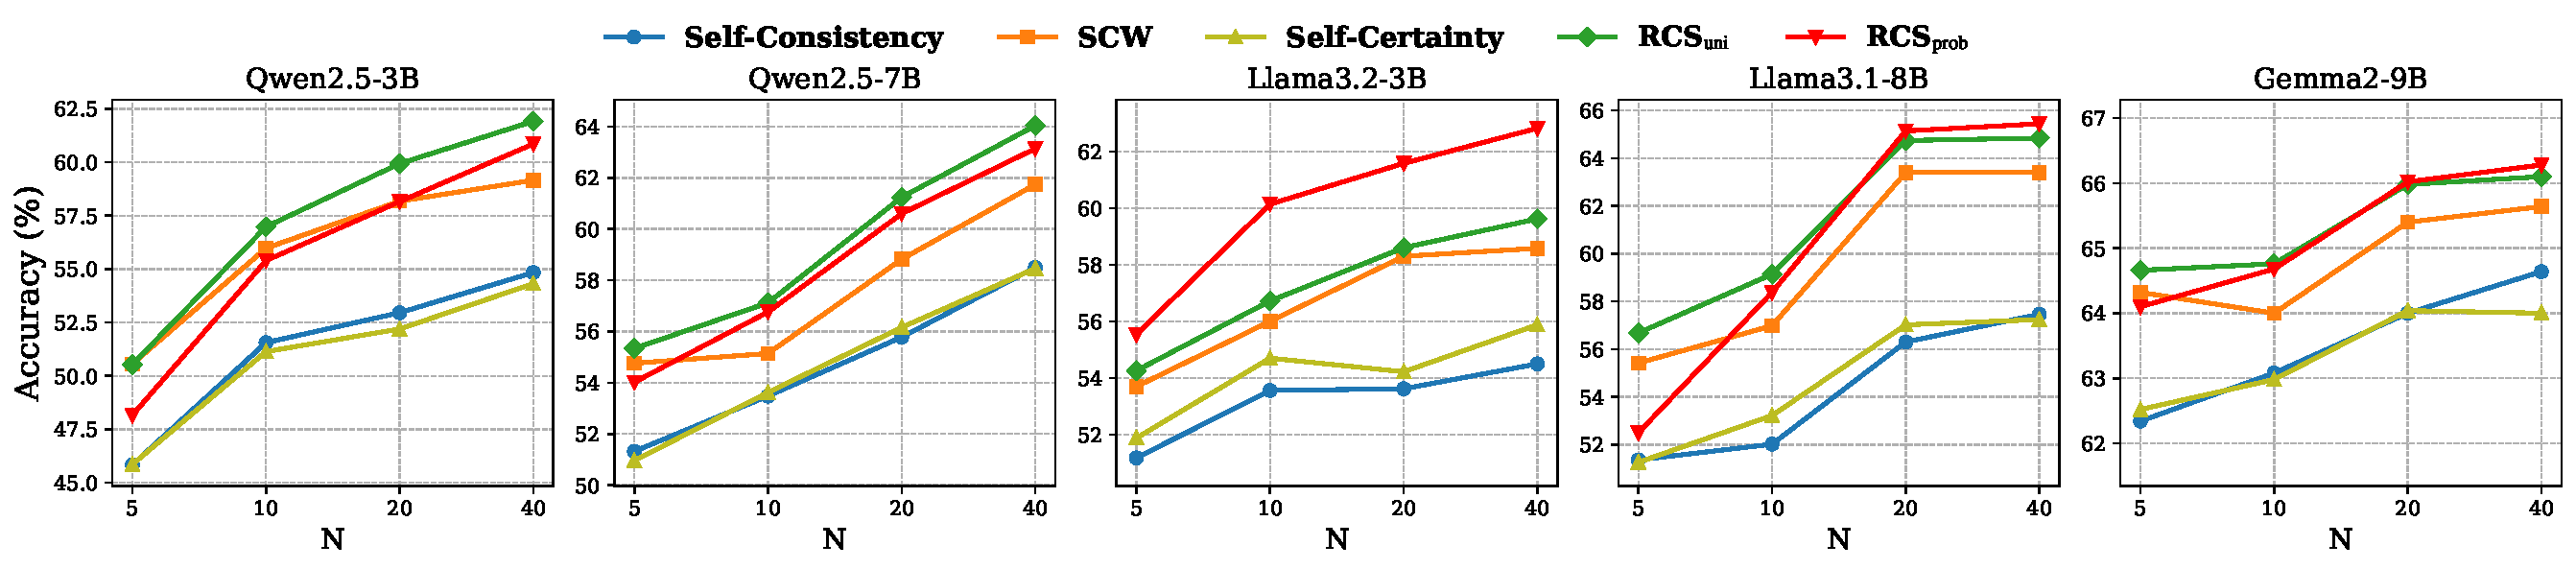
\includegraphics[width=\textwidth]{plots/scaling_methods_v6.pdf}
    \caption{
    Average performance over five benchmarks for different numbers of sampling responses $N$. Each subplot corresponds to an LLM backbone, showing how accuracy changes with increasing $N$.}
    \label{fig:scaling}
\end{figure}
% -----------
We report four RCS variants (Table~\ref{tab:rds_variants}): RCS$_\text{uni}$, RCS$_\text{freq}$, RCS$_\text{cosine}$ (per-sample cosine-similarity weights applied to final-answer embeddings), and RCS$_\text{prob}$ (using ANLL as a length-normalized probability proxy). We also report RCS$_\text{medoid}$ (uniform, unweighted) as a discrete baseline. All RCS variants use \texttt{all-MiniLM-L6-v2}~\citep{reimers2019sentence}. We sample $N{=}10$ responses (also $N{=}5,20,40$) at $T{=}1$ via vLLM~\citep{kwon2023efficient}; results are mean$\pm$std over three seeds. Additional details are in Appendix~\ref{app:details}.

% and investigate clean-answer setting in Section~\ref{sec:ablation}. 
% \paragraph{Evaluation Protocol.} For all methods, we measure accuracy (\%) between the selected answer and the ground-truth. A generation is deemed correct via exact match on long-form reasoning tasks or ROUGE-L F1 $>$ 0.3 on short-form QA tasks (SciQ, GPQA), exactly as in prior work~\citep{kuhn2023semantic, nguyen2025probabilities}. We include all model outputs, including empty or degenerate responses, to reflect real-world noisy generation settings.

% \paragraph{Sampling and Implementation.}
% We sample $N$ responses per question using multinomial sampling with temperature $T{=}1$ via vLLM~\citep{kwon2023efficient}. Unless otherwise stated, we use $N{=}10$, and additionally explore larger budgets with $N{=}5, 20, 40$. We use 5-shot prompting~\citep{brown2020language} for short-form QA and Chain-of-Thought prompting~\citep{wei2022chain} for long-form tasks. For CE, we follow the original setup and set $p{=}0.3$. 
% All RCS variants use the \texttt{all-MiniLM-L6-v2} sentence transformer~\citep{reimers2019sentence}. We report mean$\pm$std over three random seeds. Additional details are provided in Appendix~\ref{app:details}.

% ====
\subsection{Main Results}

\paragraph{RCS Consistently Outperforms Baselines.}

We report selection accuracy in Table~\ref{tab:ranking}. RCS variants consistently achieve the best performance across all settings. RCS$_\text{uni}$ and RCS$_\text{prob}$ rank first overall, outperforming the best baseline (CE) by 2--6\%. RCS$_\text{cosine}$ consistently ranks second among RCS variants (avg.\ 56.9--59.1), outperforming SCW (avg.\ 56.0--57.0) despite using the same pairwise cosine signals---demonstrating that the RCS Fréchet-mean framework extracts more value from the same information by bypassing the discrete grouping step. RCS$_\text{freq}$ outperforms SC by avoiding hard tie-breaking through soft semantic weighting.
Among baselines, CE is the strongest competitor. ModeX and SCW both underperform due to full-trajectory embedding collapse and, in SCW's case, the additional discrete-voting step that misses minority correct answers (Section~\ref{sec:embedding-collapse}).
Overall, results confirm that a unified geometric framework with flexible weighting distributions is both more expressive and more robust than fixed surface-form or trajectory-level aggregation.

% ==================SCALABILITY============================
\paragraph{RCS Scales Effectively with Increasing Sampling Budget.}\label{sec:scaling}

Figure~\ref{fig:scaling} shows performance as the number of sampled responses $N$ increases with only top methods are shown. We highlight $\text{RCS}_{\text{uni}}$ and $\text{RCS}_{\text{prob}}$, the best-performing variants from Table~\ref{tab:ranking} (full results in Appendix~\ref{app:sample-details}).
RCS consistently outperforms all baselines at larger $N$ (e.g., $N{=}20,40$), with gains up to +7\%. As $N$ increases, correct answers may remain in the minority; RCS recovers them by anchoring to the semantic center rather than to frequency, maintaining robustness even when correct outputs are sparse.




% =========================ABLATION=====================
\subsection{Ablation Study}\label{sec:ablation}

% In this section, we investigate the effects of hyperparameters, including the number of sampling responses $N$ and choice of embedding model $\mathbf{E}$. 
To reduce computational overhead, experiments are conducted using two representative models: Qwen2.5-3B and Llama3.2-3B.





\paragraph{RCS Enhances Multi-Agent Debate.}

\begin{table}[ht]
  \centering
  \caption{Performance on Arithmetics and Form.Log. with Multi-agent Debate. Best values are bolded. \textbf{R=0,1,2} indicate debate rounds, while \textbf{Avg.} denotes the average over all rounds. RCS$_\text{base}$ $\equiv$ RCS$_\text{uni}$ (uniform weighting).}
  \label{tab:mad_qwen2.5-3b}
  % \renewcommand{\arraystretch}{0.85}
  \resizebox{\columnwidth}{!}{
  \begin{tabular}{cll|cccc|cccc}
    \toprule
    \multirow{2}{*}{\textbf{Model}} 
    & \multirow{2}{*}{\textbf{Method}} 
    & \multirow{2}{*}{\textbf{N}} 
    & \multicolumn{4}{c|}{\textbf{Arithmetics}}
    & \multicolumn{4}{c}{\textbf{Form.Log.}} 
    % & \multicolumn{3}{c}{\textbf{MMLU-Pro}} 
    \\
    
    \cmidrule(lr){4-7} \cmidrule(lr){8-11} % \cmidrule(lr){9-11}
    
    & &
    & \textbf{R=0} & \textbf{R=1} & \textbf{R=2} & \textbf{Avg.}
    & \textbf{R=0} & \textbf{R=1} & \textbf{R=2} & \textbf{Avg.}
    % & \textbf{R=0} & \textbf{R=1} & \textbf{R=2} 
    \\
    
    \midrule
    % \multicolumn{8}{c}{\textbf{Qwen2.5-3B}} \\
    % \midrule

    \multirow{6}{*}{\rotatebox[origin=c]{90}{Qwen2.5-3B}}
    &
    SC & 10  
    & 94.5$\pm$4.0&	60.4$\pm$1.6	&34.6$\pm$5.8   & 63.1
    & 44.8$\pm$2.5&	35.3$\pm$2.9	&27.6$\pm$5.4   & 35.9
    % & 23.8$\pm$5.9&	22.9$\pm$5.8	&24.8$\pm$2.9 
    \\

    &
    \cellcolor{green!15}RCS$_\text{base}$ & \cellcolor{green!15}10
    & \cellcolor{green!15}94.3$\pm$3.7	&\cellcolor{green!15}59.5$\pm$4.1&\cellcolor{green!15}	34.0$\pm$11.0 & \cellcolor{green!15}62.6
    & \cellcolor{green!15}\textbf{46.0$\pm$2.3}	&\cellcolor{green!15}35.8$\pm$5.3	&\cellcolor{green!15}\textbf{28.8$\pm$6.0} & \cellcolor{green!15}\textbf{36.9}
    % & 25.4$\pm$7.4&	22.9$\pm$6.6&	24.4$\pm$5.8 
    \\
    &
    \cellcolor{green!15}RCS$_\text{freq}$ & 10\cellcolor{green!15}
    & \cellcolor{green!15}\textbf{95.2$\pm$3.6}&\cellcolor{green!15}	\textbf{61.4$\pm$1.2}	&\cellcolor{green!15}\textbf{34.7$\pm$5.4} & \cellcolor{green!15}\textbf{63.8 }
    & \cellcolor{green!15}44.8$\pm$2.8&\cellcolor{green!15}	\textbf{36.1$\pm$3.3}&\cellcolor{green!15}	28.7$\pm$5.5 & \cellcolor{green!15}36.5
    % & 24.8$\pm$5.9&	25.4$\pm$6.3&	26.0$\pm$3.9 
    \\

    \cmidrule(lr){2-11}
    &
    SC & 20  
    & 96.5$\pm$0.5&	24.8$\pm$3.0	&34.0$\pm$3.3 & 51.8
    & 42.3$\pm$0.5	&40.5$\pm$1.6	&35.7$\pm$1.6 & 39.5
    % & 23.8$\pm$1.3&	26.2$\pm$3.4	&25.7$\pm$2.7 
    \\
    & 
    \cellcolor{green!15}RCS$_\text{base}$ & 20\cellcolor{green!15}
    & \cellcolor{green!15}\textbf{97.7$\pm$1.0}	&\cellcolor{green!15}\textbf{27.3$\pm$3.2}	&\cellcolor{green!15}\textbf{34.5$\pm$5.1} & \cellcolor{green!15}\textbf{53.2} 
    & \cellcolor{green!15}\textbf{46.6$\pm$0.9}	&\cellcolor{green!15}\textbf{45.2$\pm$1.4}&	\cellcolor{green!15}\textbf{37.8$\pm$0.9} & \cellcolor{green!15}\textbf{43.2}
    % & 24.3$\pm$0.7&	27.6$\pm$6.7&	24.3$\pm$4.7 
    \\
    &
    \cellcolor{green!15}RCS$_\text{freq}$ & 20\cellcolor{green!15}
    & \cellcolor{green!15}97.2$\pm$0.3	&\cellcolor{green!15}26.0$\pm$2.2&\cellcolor{green!15}	34.3$\pm$4.0 & \cellcolor{green!15}52.5
    & \cellcolor{green!15}42.6$\pm$0.5&	\cellcolor{green!15}42.1$\pm$0.8&\cellcolor{green!15}	35.7$\pm$1.6 & \cellcolor{green!15}40.1
    % & 24.8$\pm$2.7&	25.2$\pm$6.1&	24.3$\pm$8.8 
    \\

    \midrule
    % \multicolumn{8}{c}{\textbf{Llama3.2-3B}} \\
    % \midrule
    \multirow{6}{*}{\rotatebox[origin=c]{90}{Llama3.2-3B}}
    &
    SC & 10  
    & 80.7$\pm$2.0	&85.6$\pm$10.7&	75.8$\pm$5.9 & 80.7
    & 31.3$\pm$2.9&	28.4$\pm$7.8	&29.5$\pm$7.7 & 29.7
    % & 16.2$\pm$2.5	&14.0$\pm$1.1	&14.0$\pm$2.9 
    \\
    &
    \cellcolor{green!15}RCS$_\text{base}$ & 10\cellcolor{green!15}
    & \cellcolor{green!15}79.1$\pm$4.3	&\cellcolor{green!15} \textbf{85.8$\pm$9.1}&\cellcolor{green!15}	\textbf{76.2$\pm$4.6} & \cellcolor{green!15}80.4
    & 	\cellcolor{green!15}\textbf{33.2$\pm$0.5}&\cellcolor{green!15}	\textbf{28.7$\pm$8.0}	&\cellcolor{green!15}\textbf{29.9$\pm$6.4} & \cellcolor{green!15}\textbf{30.6}
    % & 17.5$\pm$4.7	&14.9$\pm$2.0	&14.3$\pm$1.0 
    \\
    &
    \cellcolor{green!15}RCS$_\text{freq}$ & 10\cellcolor{green!15}
    & \cellcolor{green!15}\textbf{81.1$\pm$12.7}&	\cellcolor{green!15}85.6$\pm$10.0	&\cellcolor{green!15}\textbf{76.2$\pm$5.1} & \cellcolor{green!15}\textbf{81.0}
    & \cellcolor{green!15}32.1$\pm$2.9&	\cellcolor{green!15}28.6$\pm$8.3	&\cellcolor{green!15}29.5$\pm$16.6 & \cellcolor{green!15}30.1
    % & 15.6$\pm$4.7&	14.9$\pm$2.0	&12.7$\pm$1.1 
    \\

    \cmidrule(lr){2-11}
    &
    SC & 20  
    & 99.0$\pm$0.5&	72.2$\pm$4.1&	41.5$\pm$2.2 & 70.9
    & 13.2$\pm$0.5&	3.2$\pm$0.8	&3.7$\pm$1.7 & 6.7
    % & 21.4$\pm$3.4&	15.7$\pm$0.7	&13.8$\pm$2.0 
    \\
    &
    \cellcolor{green!15}RCS$_\text{base}$ & 20\cellcolor{green!15}
    & \cellcolor{green!15}99.0$\pm$1.0	&\cellcolor{green!15}\textbf{76.5$\pm$4.3}	&\cellcolor{green!15}\textbf{43.3$\pm$1.5} & \cellcolor{green!15}\textbf{72.9}
    & \cellcolor{green!15}\textbf{21.4$\pm$2.4}&\cellcolor{green!15}	\textbf{9.0$\pm$1.2}&\cellcolor{green!15}	\textbf{7.1$\pm$2.4}&\cellcolor{green!15}\textbf{12.5}
    % & 18.1$\pm$8.1	&18.1$\pm$4.0&	14.3$\pm$6.7 
    \\
    &
    \cellcolor{green!15}RCS$_\text{freq}$ & 20\cellcolor{green!15}
    & \cellcolor{green!15}\textbf{99.2$\pm$0.8}	&\cellcolor{green!15}73.8$\pm$3.8&\cellcolor{green!15}	42.5$\pm$2.6 & \cellcolor{green!15}71.8
    & \cellcolor{green!15}15.6$\pm$1.7	&\cellcolor{green!15}4.2$\pm$0.5&\cellcolor{green!15}	3.7$\pm$0.9 & \cellcolor{green!15}7.8
    % & 19.0$\pm$2.7&	15.7$\pm$3.4&	13.8$\pm$0.7 
    \\

    \bottomrule
  \end{tabular}}
\end{table}
% ------------
% ------
% =================
\begin{table*}[t]
\centering
\caption{Performance under (a) black-box setting ($N{=}$10) and (b) complexity comparison.}
\label{tab:clean-blackbox-complexity}
\resizebox{\linewidth}{!}{
\begin{tabular}{c c}
% ================= LEFT TABLE (a) =================
% \begin{minipage}[t]{0.70\linewidth}
% \centering
% \caption*{\vspace{1pt}(a)}
% \resizebox{\linewidth}{!}{
% \begin{tabular}{l|cc|cc}
% \toprule
% \multirow{2}{*}{\textbf{Method}} 
% & \multicolumn{2}{c|}{\textbf{Qwen2.5-3B}} 
% & \multicolumn{2}{c}{\textbf{Llama3.2-3B}} \\
% \cmidrule(lr){2-3} \cmidrule(lr){4-5}
% & \textbf{Arithmetics} & \textbf{Form.Log.} 
% & \textbf{Arithmetics} & \textbf{Form.Log.} \\
% \midrule
% NLL  & 54.2$\pm$4.3 & 29.6$\pm$5.6 & 87.0$\pm$1.0 & 38.6$\pm$4.4 \\
% ANLL & 54.0$\pm$4.0 & 29.9$\pm$6.2 & 89.5$\pm$2.3 & 38.9$\pm$5.6 \\
% SC   & 96.7$\pm$1.2 & 46.6$\pm$1.7 & 98.0$\pm$1.3 & 36.2$\pm$3.2 \\
% CE   & 96.5$\pm$0.9 & 48.4$\pm$1.1 & 97.8$\pm$1.3 & 37.8$\pm$2.9 \\
% \rowcolor{green!15}RCS$_{\text{medoid}}$ & \textbf{97.2$\pm$0.6} & 48.9$\pm$1.2 & \textbf{98.3$\pm$0.8} & 36.5$\pm$2.9 \\
% \rowcolor{green!15}RCS$_{\text{uni}}$  & 95.5$\pm$1.3 & 49.2$\pm$0.8 & 98.2$\pm$1.0 & 37.0$\pm$3.3 \\
% \rowcolor{green!15}RCS$_{\text{freq}}$ & 96.8$\pm$0.6 & \textbf{49.7$\pm$0.9} & \textbf{98.3$\pm$0.8} & 37.0$\pm$2.0 \\
% \rowcolor{green!15}RCS$_{\text{prob}}$ & 94.3$\pm$1.9 & 48.4$\pm$0.8 & 97.7$\pm$1.0 & \textbf{40.2$\pm$4.8} \\
% \bottomrule
% \end{tabular}}

% \end{minipage}

\begin{minipage}[t]{0.75\linewidth}
\centering
    \caption*{(a)}

\label{tab:blackbox}
\resizebox{\linewidth}{!}{
\begin{tabular}{l|cccc|c}
\toprule
\textbf{Method} & \textbf{GPQA} & \textbf{MMLU-Pro} & \textbf{BBH-Date} & \textbf{BBH-Navigate} & {\textbf{Avg.}}\\
\midrule
SC  & 13.1 & 47.6 & 76.8 & 39.2 & 44.2\\
\rowcolor{green!15}RCS$_\text{medoid}$ & \textbf{14.6} & \textbf{48.6} & 76.4 & 39.2 & 44.7\\
\rowcolor{green!15}RCS$_\text{base}$   & 14.1 & \textbf{48.6} & \textbf{78.0} & 40.2 & \textbf{45.2}\\
\rowcolor{green!15}RCS$_\text{freq}$   & 13.6 & 47.6 & 77.6 & \textbf{41.2} & 45.0\\
\bottomrule
\end{tabular}}
\end{minipage}


&

% ================= RIGHT SIDE (b + c stacked) =================
\begin{minipage}[t]{0.22\linewidth}
\centering

% -------- (b) Blackbox table --------
% \caption*{(b)}

% \label{tab:blackbox}
% \resizebox{\linewidth}{!}{
% \begin{tabular}{l|cc}
% \toprule
% \textbf{Method} & \textbf{AIME25} & \textbf{MMLU-Pro} \\
% \midrule
% SC  & \textbf{6.7} & 47.6 \\
% \rowcolor{green!15}RCS$_\text{medoid}$ & \textbf{6.7} & \textbf{48.6} \\
% \rowcolor{green!15}RCS$_\text{base}$   & \textbf{6.7} & \textbf{48.6} \\
% \rowcolor{green!15}RCS$_\text{freq}$   & \textbf{6.7} & 47.6 \\
% \bottomrule
% \end{tabular}}

% \vspace{1pt}

% -------- (c) Complexity table --------
\caption*{(b)}

\label{tab:complexity}
\resizebox{\linewidth}{!}{
\begin{tabular}{l c}
\toprule
\textbf{Method} & \textbf{Complexity} \\
\midrule
NLL, ANLL & $\mathcal{O}(NL)$ \\
SC & $\mathcal{O}(N)$ \\
CE & $\mathcal{O}(NL)$ \\
ModeX & $\mathcal{O}(N^2L + N^3)$\\
SCW & $\mathcal{O}(N^2d)$ \\
\rowcolor{green!15}RCS$_\text{medoid}$ & $\mathcal{O}(N^2d)$ \\
\rowcolor{green!15}RCS$_\text{uni/freq}$ & $\mathcal{O}(Nd)$ \\
\rowcolor{green!15}RCS$_\text{prob}$ & $\mathcal{O}(N(d + L))$ \\
\rowcolor{green!15}RCS$_\text{cosine}$ & $\mathcal{O}(N^2d)$ \\
\bottomrule
\end{tabular}
}

\end{minipage}

\end{tabular}
}
\end{table*}

% -----------


\begin{figure*}[ht]
\centering
\fcolorbox{black}{white}{%
\resizebox{\linewidth}{!}{%
\begin{tabular}{l}

% ===================== Arithmetics =====================
\textbf{Arithmetics} - Ground Truth: \textbf{10} \\[0.5em]

\fcolorbox{gray}{blue!5!white}{%
\parbox{0.98\textwidth}{
\centering
\textbf{A1:} 10 \hspace{8mm}
\textbf{A2:} 10 \hspace{8mm}
\textbf{A3:} 15 \hspace{8mm}
\textbf{A4:} 15 \hspace{8mm}
\textbf{A5:} 5
}
} \\[0.8em]

\begin{tabular}{c c}

\fcolorbox{gray}{blue!5!white}{%
\parbox{0.45\linewidth}{
\centering
Self-Consistency fails to clearly distinguish between 10 and 15 (\textcolor{red}{\ding{55}}).
}
}
&
\fcolorbox{gray}{blue!5!white}{%
\parbox{0.45\linewidth}{
\centering
RCS selects \textcolor{green}{10} (\textcolor{green}{\ding{51}}), as the outlier (5) shifts the center toward A1/A2.
}
}
\end{tabular}

% ===================== DIVIDER =====================
\\[1.2em]
\noalign{\hrule height 0.5pt}
\\[-0.3em]

% ===================== Formal Logic =====================
\textbf{Form.Log.} - Ground Truth: \textbf{(B)} \\[0.5em]

\fcolorbox{gray}{blue!5!white}{%
\parbox{0.98\textwidth}{
\centering
\textbf{A1:} (A) \hspace{8mm}
\textbf{A2:} (A) \hspace{8mm}
\textbf{A3:} (B) \hspace{8mm}
\textbf{A4:} (B) \hspace{8mm}
\textbf{A5:} (C)
}
} \\[0.8em]

\begin{tabular}{c c}

\fcolorbox{gray}{blue!5!white}{%
\parbox{0.45\linewidth}{
\centering
Self-Consistency struggles to choose between (A) and (B) (\textcolor{red}{\ding{55}}).
}
}
&
\fcolorbox{gray}{blue!5!white}{%
\parbox{0.45\linewidth}{
\centering
RCS selects \textcolor{green}{(B)} (\textcolor{green}{\ding{51}}), as the outlier (C) shifts the center toward (B).
}
}
\end{tabular}

\end{tabular}
}%
}
\caption{Qualitative examples showing RCS recovers correct answers more reliably than SC.}\label{fig:qualitative}
\end{figure*}
% --------------


\begin{figure*}[!t]
    \centering
    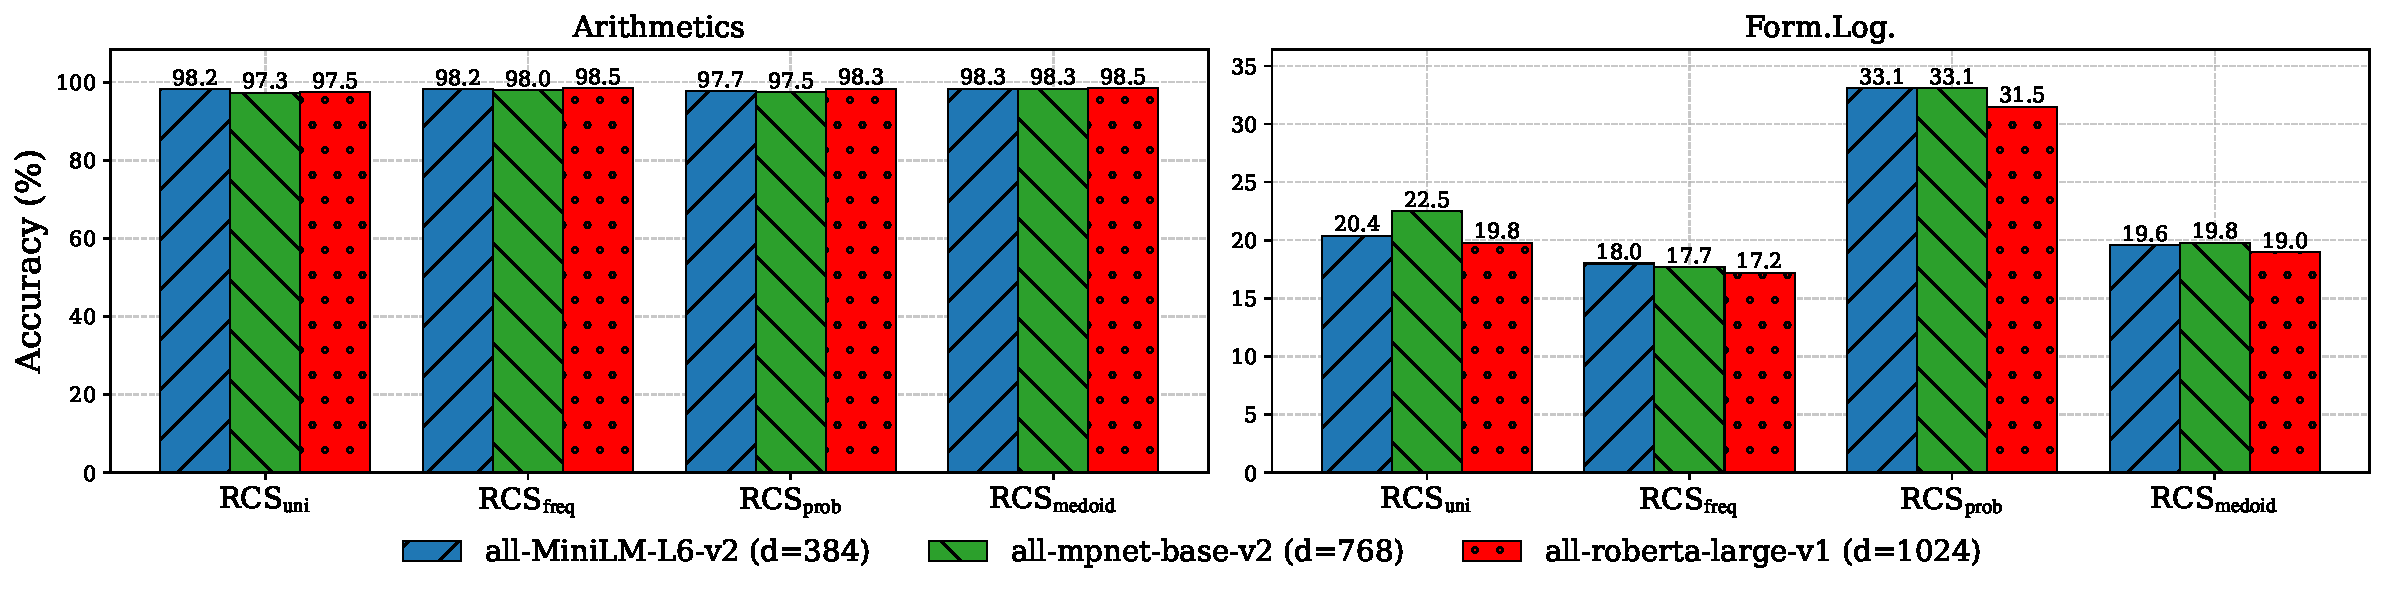
\includegraphics[width=\linewidth]{plots/abl_llama3.2-3b_embedding_v3.pdf}
    \caption{
    Effect of encoders on Llama3.2-3B. Results for Qwen2.5-3B are in Appendix Figure~\ref{fig:embed_qwen2.5-3b}.
    }
    \label{fig:embed_llama3.2-3b}
\end{figure*}

%------------
\begin{figure*}[!t]
    \centering
    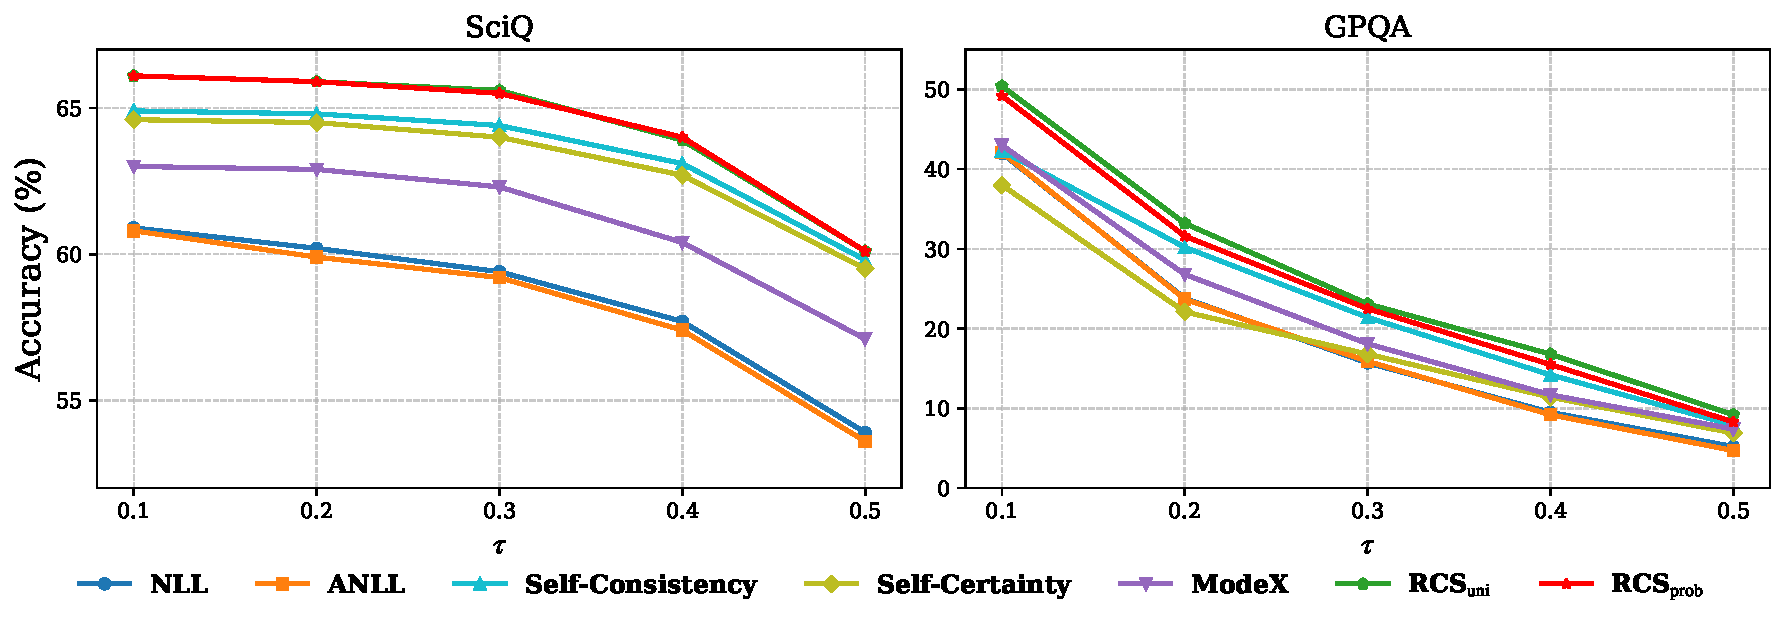
\includegraphics[width=\linewidth]{plots/abl_qwen2.5-3b_threshold_v5.pdf}
    \caption{
    Effect of varying $\tau$ using Qwen2.5-3B. Results for Llama3.2-3B are in Appendix Figure~\ref{fig:threshold_llama3.2-3b}.
    }
    \label{fig:threshold_qwen2.5-3b}
\end{figure*}
% ----------



We further evaluate RCS as a drop-in replacement for majority voting in multi-agent debate~\citep{du2023improving, choi2025debate} under a fully black-box setting with $N{=}10,20$ agents and $R{=}2$ rounds. We report RCS$_\text{base}$ and RCS$_\text{freq}$ (Table~\ref{tab:mad_qwen2.5-3b}), which are computationally efficient and do not require access to model internals.
Increasing the number of agents to $N{=}20$ consistently degrades performance across debate rounds, particularly on Llama3.2-3B, suggesting that naive scaling introduces additional variability that destabilizes reasoning~\citep{nguyen2026hear}. In contrast, RCS improves performance by 1--2\% on average, with larger gains at $N{=}20$, highlighting its robustness when aggregation becomes more challenging.

% Notably, increasing the number of agents to $N{=}20$ leads to a consistent performance drop across main debate rounds ($R{=}1,2$), particularly on Llama3.2-3B. This suggests that naively scaling up the number of agents in multi-agent debate may not always be beneficial, as it can introduce additional variability that degrades reasoning quality and destabilizes subsequent debate updates~\citep{nguyen2026hear}. 
% In contrast, RCS consistently improves performance by 1--2\% on average, with more pronounced gains at $N{=}20$, indicating its robustness in settings where answer distributions are less structured and effective aggregation becomes critical.

% \begin{table}[t]
% \centering
% \caption{Performance on Arithmetics and Form.Log. with Multi-agent Debate on Qwen2.5-3B. Best values are bolded. $R{=}0,1,2$ indicate debate rounds. Similar results for Llama3.2-3B are provided in Appendix Table~\ref{tab:mad_llama3.2-3b}.}
% \label{tab:mad_qwen2.5-3b}

% \begin{tabular}{l l|ccc}
% \toprule
% \textbf{Dataset} & \textbf{Method} & \textbf{R=0} & \textbf{R=1} & \textbf{R=2} \\
% \midrule

% \multirow{3}{*}{Arithmetics}
% & SC
% & 98.3$\pm$0.6 & 76.7$\pm$0.8 & \textbf{38.8$\pm$3.5} \\

% & RCS$_\text{base}$
% & \textbf{98.5$\pm$0.5} & \textbf{77.0$\pm$0.5} & \textbf{38.8$\pm$4.0} \\

% & RCS$_\text{freq}$
% & 98.3$\pm$0.8 & 76.7$\pm$0.6 & \textbf{38.8$\pm$3.5} \\

% \midrule

% \multirow{3}{*}{Form.Log.}
% & SC
% & 43.4$\pm$4.8 & 33.9$\pm$2.3 & 26.5$\pm$1.2 \\

% & RCS$_\text{base}$
% & \textbf{44.7$\pm$2.8} & \textbf{35.7$\pm$2.1} & 26.7$\pm$1.7 \\

% & RCS$_\text{freq}$
% & 44.4$\pm$3.2 & 35.4$\pm$2.4 & \textbf{27.0$\pm$1.6} \\

% \bottomrule
% \end{tabular}
% \end{table}

% \begin{table}[t]
% \centering
% \caption{Performance under (a) Multi-agent Debate (MAD) on Qwen2.5-3B and (b) Clean-answer setting. Best values are bolded. For MAD, $R{=}0,1,2$ indicate debate rounds and similar results for Llama3.2-3B are provided in Appendix Table~\ref{tab:mad_llama3.2-3b}. }
% \label{tab:mad_clean}

% \begin{minipage}[t]{0.45\linewidth}
% \centering
% \caption*{(a)}
% \resizebox{\linewidth}{!}{
% \begin{tabular}{l l|ccc}
% \toprule
% \textbf{Dataset} & \textbf{Method} & \textbf{R=0} & \textbf{R=1} & \textbf{R=2} \\
% \midrule

% \multirow{3}{*}{Arithmetics}
% & SC
% & 98.3$\pm$0.6 & 76.7$\pm$0.8 & \textbf{38.8$\pm$3.5} \\

% & RCS$_\text{base}$
% & \textbf{98.5$\pm$0.5} & \textbf{77.0$\pm$0.5} & \textbf{38.8$\pm$4.0} \\

% & RCS$_\text{freq}$
% & 98.3$\pm$0.8 & 76.7$\pm$0.6 & \textbf{38.8$\pm$3.5} \\

% \midrule

% \multirow{3}{*}{Form.Log.}
% & SC
% & 43.4$\pm$4.8 & 33.9$\pm$2.3 & 26.5$\pm$1.2 \\

% & RCS$_\text{base}$
% & \textbf{44.7$\pm$2.8} & \textbf{35.7$\pm$2.1} & 26.7$\pm$1.7 \\

% & RCS$_\text{freq}$
% & 44.4$\pm$3.2 & 35.4$\pm$2.4 & \textbf{27.0$\pm$1.6} \\

% \bottomrule
% \end{tabular}
% }
% \end{minipage}
% \hfill
% \begin{minipage}[t]{0.53\linewidth}
% \centering
% \caption*{(b)}
% \resizebox{\linewidth}{!}{
%   \begin{tabular}{l|cc|cc}
%     \toprule
%     \multirow{2}{*}{\textbf{Method}} 
%     & \multicolumn{2}{c|}{\textbf{Qwen2.5-3B}} 
%     & \multicolumn{2}{c}{\textbf{Llama3.2-3B}} \\
%     \cmidrule(lr){2-3} \cmidrule(lr){4-5}
%     & \textbf{Arithmetics} & \textbf{Form.Log.} 
%     & \textbf{Arithmetics} & \textbf{Form.Log.} \\
%     \midrule
%     NLL  & 54.2$\pm$4.3 & 29.6$\pm$5.6 & 87.0$\pm$1.0 & 38.6$\pm$4.4 \\
%     ANLL & 54.0$\pm$4.0 & 29.9$\pm$6.2 & 89.5$\pm$2.3 & 38.9$\pm$5.6 \\
%     SC   & 96.7$\pm$1.2 & 46.6$\pm$1.7 & 98.0$\pm$1.3 & 36.2$\pm$3.2 \\
%     CE   & 96.5$\pm$0.9 & 48.4$\pm$1.1 & 97.8$\pm$1.3 & 37.8$\pm$2.9 \\
%     \rowcolor{green!15} RCS$_{\text{medoid}}$ & \textbf{97.2$\pm$0.6} & 48.9$\pm$1.2 & 98.3$\pm$0.8 & 36.5$\pm$2.9 \\
%     \rowcolor{green!15} RCS$_{\text{uni}}$  & 95.5$\pm$1.3 & 49.2$\pm$0.8 & 98.2$\pm$1.0 & 37.0$\pm$3.3 \\
%     \rowcolor{green!15} RCS$_{\text{freq}}$ & 96.8$\pm$0.6 & \textbf{49.7$\pm$0.9} & \textbf{98.3$\pm$0.8} & 37.0$\pm$2.0 \\
%     \rowcolor{green!15} RCS$_{\text{prob}}$ & 94.3$\pm$1.9 & 48.4$\pm$0.8 & 97.7$\pm$1.0 & \textbf{40.2$\pm$4.8} \\
%     \bottomrule
%   \end{tabular}}
% \end{minipage}
% \end{table}

% \paragraph{Performance Under Clean-Answer Setting.}
% We observe that empty or degenerate responses often occur in long-form reasoning tasks. For fair comparison, we report results under a clean-answer setting, where blank or null responses are excluded from selection (Table~\ref{tab:clean-blackbox-complexity}a).
% % Removing blank answers slightly reduces performance, particularly on mathematical datasets. 
% % This suggests that blank responses are not purely noise, but may carry informative signals about model uncertainty.
% RCS-based methods remain the best-performing approaches across all settings, although the performance gap becomes smaller compared to the default setting. 
% This indicates that competing methods are more sensitive to noisy contexts, where the presence of invalid responses degrades their effectiveness more significantly.
% Notably, the advantage of RCS is more pronounced on the Form.Log., with an average improvement of around 1--2\% over the second-best method. 
% This may be attributed to the richer semantic structure of symbolic outputs (e.g. (A)), where embedding-based aggregation can better exploit high-dimensional information compared to purely numerical answers.

% \begin{table}[t]
%   \centering
%   \caption{Performance on Arithmetics and Form.Log. under clean-answer setting. Best values are bolded.}
%   \label{tab:clean}
%   % \resizebox{\columnwidth}{!}{
%   \begin{tabular}{l|cc|cc}
%     \toprule
%     \multirow{2}{*}{\textbf{Method}} 
%     & \multicolumn{2}{c|}{\textbf{Qwen2.5-3B}} 
%     & \multicolumn{2}{c}{\textbf{Llama3.2-3B}} \\
%     \cmidrule(lr){2-3} \cmidrule(lr){4-5}
%     & \textbf{Arithmetics} & \textbf{Form.Log.} 
%     & \textbf{Arithmetics} & \textbf{Form.Log.} \\
%     \midrule
%     NLL  & 54.2$\pm$4.3 & 29.6$\pm$5.6 & 87.0$\pm$1.0 & 38.6$\pm$4.4 \\
%     ANLL & 54.0$\pm$4.0 & 29.9$\pm$6.2 & 89.5$\pm$2.3 & 38.9$\pm$5.6 \\
%     SC   & 96.7$\pm$1.2 & 46.6$\pm$1.7 & 98.0$\pm$1.3 & 36.2$\pm$3.2 \\
%     CE   & 96.5$\pm$0.9 & 48.4$\pm$1.1 & 97.8$\pm$1.3 & 37.8$\pm$2.9 \\
%     \rowcolor{green!15} RCS$_{\text{medoid}}$ & \textbf{97.2$\pm$0.6} & 48.9$\pm$1.2 & 98.3$\pm$0.8 & 36.5$\pm$2.9 \\
%     \rowcolor{green!15} RCS$_{\text{uni}}$  & 95.5$\pm$1.3 & 49.2$\pm$0.8 & 98.2$\pm$1.0 & 37.0$\pm$3.3 \\
%     \rowcolor{green!15} RCS$_{\text{freq}}$ & 96.8$\pm$0.6 & \textbf{49.7$\pm$0.9} & \textbf{98.3$\pm$0.8} & 37.0$\pm$2.0 \\
%     \rowcolor{green!15} RCS$_{\text{prob}}$ & 94.3$\pm$1.9 & 48.4$\pm$0.8 & 97.7$\pm$1.0 & \textbf{40.2$\pm$4.8} \\
%     \bottomrule
%   \end{tabular}
%   % }
% \end{table}


\paragraph{RCS Improves Under Fully Black-box Setting.}
We further evaluate a fully black-box setting using Cohere (\textit{command-a-03-2025}) on GPQA, MMLU-Pro, and BigBenchHard (Table~\ref{tab:clean-blackbox-complexity}a). RCS outperforms traditional Self-Consistency, with RCS$\text{base}$ achieving the best performance, yielding +1\% average improvement. This highlights the advantage of RCS in capturing consistency beyond simple frequency-based selection.

% \begin{table}[t]
%   \centering
%   \caption{Performance across methods under fully blackbox setting. Best values are bolded.}
%   \label{tab:blackbox}
%   % \resizebox{\columnwidth}{!}{
%   \begin{tabular}{l|cc}
%     \toprule
%     {\textbf{Method}} 
%     & {\textbf{AIME25}} 
%     & {\textbf{MMLU-Pro}} \\
%     \midrule
%     SC  & \textbf{6.7} & 47.6 \\
%     \rowcolor{green!15} RCS$_\text{medoid}$& \textbf{6.7} & \textbf{48.6} \\
%     \rowcolor{green!15} RCS$_\text{base}$ & \textbf{6.7} & \textbf{48.6} \\
%     \rowcolor{green!15} RCS$_\text{freq}$   & \textbf{6.7} & 47.6 \\
%     \bottomrule
%   \end{tabular}
%   % }
% \end{table}

% \begin{table}[t]
% \centering
% \caption{Complexity comparison (a) and performance under fully black-box setting (b).}
% \label{tab:complexity_blackbox}

% \begin{minipage}[t]{0.48\linewidth}
% \centering
% \caption*{(a)}
% \begin{tabular}{l|cc}
% \toprule
% \textbf{Method} & \textbf{AIME25} & \textbf{MMLU-Pro} \\
% \midrule
% SC & 6.7 & 47.6 \\
% RCS$_\text{medoid}$ & 6.7 & \textbf{48.6} \\
% RCS$_\text{base}$ & 6.7 & \textbf{48.6} \\
% RCS$_\text{freq}$ & 6.7 & 47.6 \\
% \bottomrule
% \end{tabular}
% \end{minipage}
% \hfill
% \begin{minipage}[t]{0.48\linewidth}
% \centering
% \caption*{(b)}
% \begin{tabular}{l c}
% \toprule
% \textbf{Method} & \textbf{Complexity} \\
% \midrule
% NLL, ANLL, SC & $\mathcal{O}(N)$ \\
% % Self-Consistency (SC) & $\mathcal{O}(N)$ \\
% Self-Certainty (CE) & $\mathcal{O}(N L V)$ \\
% RCS$_\text{medoid}$ & $\mathcal{O}(N^2 d)$ \\
% RCS$_\text{uni/freq/prob}$ & $\mathcal{O}(N d)$ \\
% \bottomrule
% \end{tabular}
% \end{minipage}
% \end{table}

\paragraph{Complexity Analysis.}\label{sec:complexity}

We report computational complexity in Table~\ref{tab:clean-blackbox-complexity}b, where $d$, $L$, and $|V|$ denote embedding dimension, sequence length, and vocabulary size.
NLL and ANLL scale as $\mathcal{O}(NL)$ due to token-level scoring, while SC is $\mathcal{O}(N)$ since it only performs frequency counting over final answers. More expressive methods such as CE and ModeX capture richer semantic or structural dependencies but incur higher costs due to full token-level distributions or pairwise interactions.
In contrast, RCS variants (e.g., RCS$_\text{uni}$) avoid pairwise comparisons by estimating a semantic center and dispersion in $\mathcal{O}(Nd)$, achieving a favorable trade-off between efficiency and semantic expressiveness.

\paragraph{Qualitative Example.}\label{sec:qualitative}
We present two qualitative examples from Arithmetics and Form.Log. (Figure~\ref{fig:qualitative}), using $N{=}5$ samples for Self-Consistency and RCS$_\text{uni}$ for simplicity. 
Self-Consistency fails when majority responses are misleading, whereas RCS$_\text{uni}$ correctly recovers the answer by leveraging informative minority samples. This highlights the robustness of RCS in aggregating diverse outputs under noisy sampling.


% \begin{table}[t]
% \centering
% \caption{Computational complexity comparison. $N$ is the number of samples, $d$ is the embedding dimension, $L$ is the sequence length, and $V$ is the vocabulary size.}
% \label{tab:complexity}
% \begin{tabular}{l c}
% \toprule
% \textbf{Method} & \textbf{Complexity} \\
% \midrule
% NLL, ANLL & $\mathcal{O}(N)$ \\%& Per-sequence likelihood scoring \\
% Self-Consistency (SC) & $\mathcal{O}(N)$ \\%& Frequency counting \\
% Self-Certainty (CE) & $\mathcal{O}(N L V)$ \\%& Token-level distributions + aggregation \\
% RCS$_\text{medoid}$ & $\mathcal{O}(N^2 d)$ \\%& Pairwise distances \\
% RCS$_\text{uni}$, RCS$_\text{freq}$, RCS$_\text{prob}$ \\%& $\mathcal{O}(Nd)$ & Center + distances in embedding space \\
% \bottomrule
% \end{tabular}
% \end{table}


% ============
% \begin{figure*}[t]
%     \centering

%     \begin{minipage}[t]{0.51\linewidth}
%         \centering
%         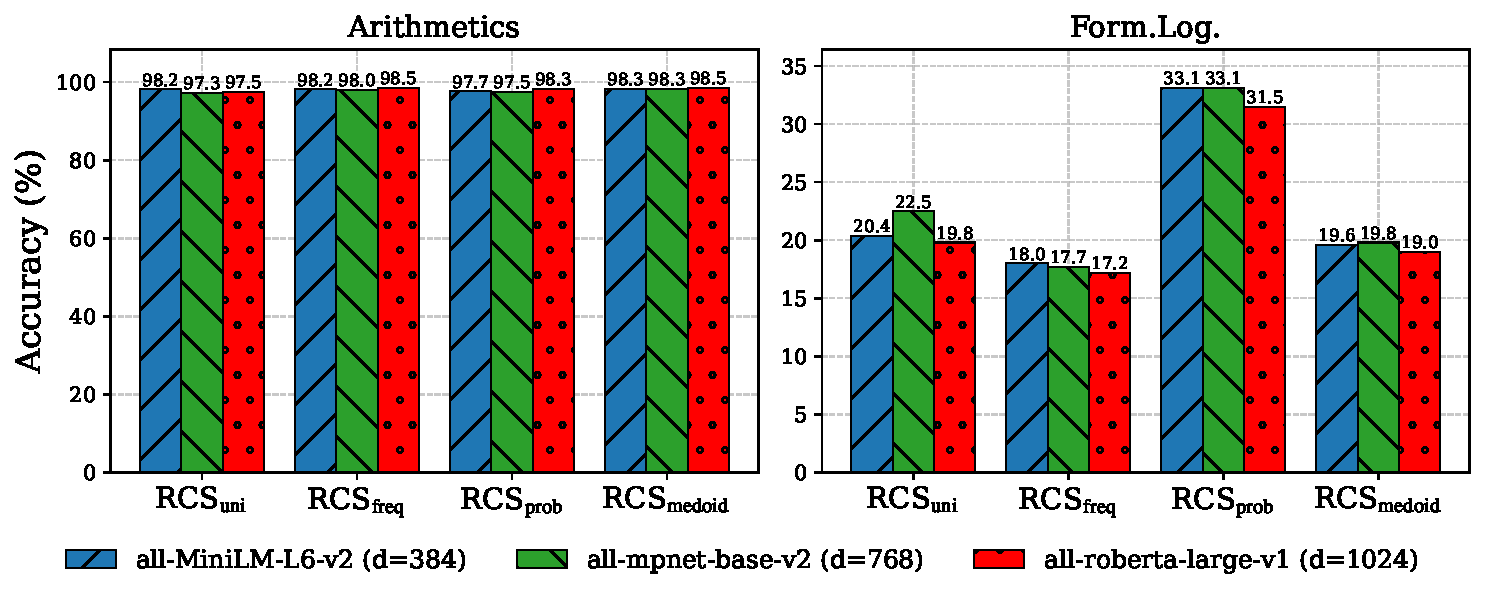
\includegraphics[width=\linewidth]{plots/abl_llama3.2-3b_embedding_v4.pdf}
%         \caption*{(a)}
%     \end{minipage}
%     \hfill
%     \begin{minipage}[t]{0.48\linewidth}
%         \centering
%         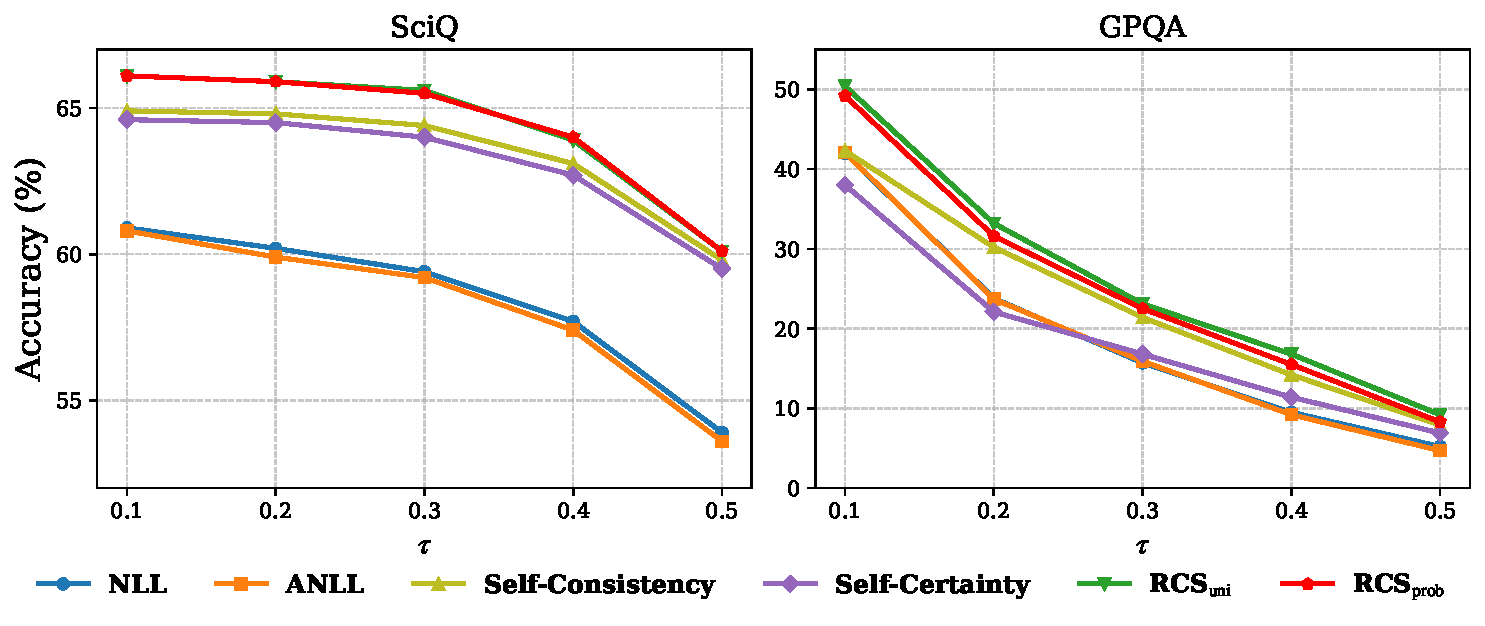
\includegraphics[width=\linewidth]{plots/abl_qwen2.5-3b_threshold_v4.pdf}
%         \caption*{(b)}
%     \end{minipage}

%     \caption{
%     (a) Effect of the sentence embedding model on Arithmetics and Form.Log. using Llama3.2-3B. 
%     (b) Performance on SciQ and GPQA when varying correctness threshold ($\tau$) using Qwen2.5-3B. 
%     Additional results are provided in Appendix Figures~\ref{fig:embed_qwen2.5-3b} and~\ref{fig:threshold_llama3.2-3b}.
%     }
%     \label{fig:embed_threshold}
% \end{figure*}
\paragraph{Analysis Of Design Choices.}
We analyze the impact of several design choices in RCS. 
% and provide qualitative examples to further illustrate its behavior. 
% \textbf{(1) Qualitative Example.}\label{sec:qualitative} We present two qualitative examples from Arithmetics and Form.Log. (Figure~\ref{fig:qualitative}), using $N{=}5$ samples for Self-Consistency and RCS$_\text{uni}$ for simplicity. 
% Self-Consistency fails when majority responses are misleading, whereas RCS$_\text{uni}$ correctly recovers the answer by leveraging informative minority samples. This highlights the robustness of RCS in aggregating diverse outputs under noisy sampling.
\textbf{(1) Effect Of Embedding Models:} In Figure~\ref{fig:embed_llama3.2-3b}, we compare three sentence transformers of increasing capacity. 
% : \texttt{all-MiniLM-L6-v2}, \texttt{all-mpnet-base-v2}, and \texttt{all-roberta-large-v1}. 
Results show minimal variation across models. This stability is especially evident on Arithmetics, where answers are numeric. On Form.Log., we observe a slight drop with \texttt{all-roberta-large-v1}, particularly for the probability-based variant, suggesting that higher embedding capacity does not necessarily improve semantic alignment in this setting. \textbf{(2) Effect Of Correctness Threshold:} Figure~\ref{fig:threshold_qwen2.5-3b} reports performance on SciQ and GPQA under varying correctness thresholds. We focus on \textsc{RCS}$_{\text{uni}}$ and \textsc{RCS}$_{\text{prob}}$, which consistently achieve the best results as the ROUGE-F1 threshold increases from 0.1 to 0.5, particularly within the common range of 0.2--0.4. 
% This demonstrates RCS's robustness to threshold selection. 
\textbf{(3) Effect of Full-Trajectory Embeddings:}\label{sec:embedding-collapse} A natural extension of RCS is to use full generation trajectories instead of final-answer embeddings. However, this leads to an \textit{embedding collapse} effect, where candidates become less distinguishable due to shared prefixes and redundant reasoning.
We compare this variant with final-answer embeddings (Appendix Figures~\ref{fig:full_qwen2.5-3b} and~\ref{fig:full_llama3.2-3b}) and observe consistent performance drops. This suggests that intermediate tokens introduce noise and weaken discriminative signals, while final answers provide a more compact and task-relevant representation. % These results support our design choice.
This collapse issue also affects methods that operate on full trajectories: ModeX applies spectral clustering over complete reasoning traces, while SCW~\citep{jain2023sc} embeds full reasoning paths and groups pairwise cosine-similarity scores by unique trajectory. Although SCW's similarity-based aggregation provides an implicit outlier-down-weighting effect, shared prefixes still cause representations to collapse, and the discrete grouping-by-trajectory step can miss minority correct answers. RCS avoids both issues by restricting embeddings to the extracted final answer and ranking all candidates continuously via the weighted Fréchet mean.

% \paragraph{Effect Of Embedding Models.}

% In Figure~\ref{fig:embed_llama3.2-3b}, we compare three sentence transformers of increasing capacity: \texttt{all-MiniLM-L6-v2}, \texttt{all-mpnet-base-v2}, and \texttt{all-roberta-large-v1}. Results show minimal variation across models. This stability is especially evident on Arithmetics, where answers are numeric. On Form.Log., we observe a slight drop with \texttt{all-roberta-large-v1}, particularly for the probability-based variant, suggesting that higher embedding capacity does not necessarily improve semantic alignment in this setting.

% \paragraph{Effect Of Correctness Threshold.}

% Figure~\ref{fig:threshold_qwen2.5-3b} reports performance on SciQ and GPQA under varying correctness thresholds. We focus on \textsc{RCS}$_{\text{uni}}$ and \textsc{RCS}$_{\text{prob}}$, which consistently achieve the best results as the ROUGE-F1 threshold increases from 0.1 to 0.5, particularly within the common range of 0.2--0.4. This demonstrates RCS's robustness to threshold selection.

% % Figure~\ref{fig:threshold_qwen2.5-3b} reports performance on SciQ and GPQA under varying correctness thresholds. We focus on \textsc{RCS}$_{\text{uni}}$ and \textsc{RCS}$_{\text{prob}}$, the two best-performing variants among our methods. As the ROUGE-F1 threshold increases from 0.1 to 0.5, both variants consistently achieve the strongest results across datasets, particularly within the commonly used range of 0.1–0.4. This demonstrates the robustness of our approach to threshold selection. 
% % Full results are provided in Appendix Table~\ref{tab:threshold_full}.


% \paragraph{Effect of Full-Trajectory Embeddings.}\label{sec:embedding-collapse}

% A natural extension of RCS is to use full generation trajectories instead of final-answer embeddings. However, this leads to an \textit{embedding collapse} effect, where candidates become less distinguishable due to shared prefixes and redundant reasoning.
% We compare this variant with final-answer embeddings (Appendix Figures~\ref{fig:full_qwen2.5-3b} and~\ref{fig:full_llama3.2-3b}) and observe consistent performance drops. This suggests that intermediate tokens introduce noise and weaken discriminative signals, while final answers provide a more compact and task-relevant representation. These results support our design choice.

% \section{Theoretical Analysis}
We provide a theoretical analysis showing that RCS is strictly superior to majority voting (self-consistency) under a Gaussian generative model on the embedding space.

\paragraph{Assumption of Gaussian Distribution.}
We model the embedding space \(\mathbb{R}^d\) (\(d \gg 1\)) where the \emph{embeddings} of the generated answers are given by
\begin{align}
\mathbf{u}_i = \mathbf{c}^* + \boldsymbol{\varepsilon}_i, \quad \boldsymbol{\varepsilon}_i \sim \mathcal{N}(\mathbf{0}, \sigma^2 \mathbf{I}), \quad i.i.d.,
\end{align}
with \(\mathbf{c}^*\) the unknown true semantic center (embedding of the highest-quality answer) and \(\boldsymbol{\varepsilon}_i\) capturing semantic noise such as paraphrasing or minor hallucinations. The discrete answers \(a_i\) themselves are produced by the LLM; the Gaussian assumption applies directly to their embeddings (the space relevant for RCS). Answer quality is inversely related to noise magnitude:
\[
Q_i = Q(a_i | x) \propto -\|\boldsymbol{\varepsilon}_i\|_2.
\]
The distribution \(P{=}\{p_i\}_{i=1}^N\) can be uniform, frequency-weighted, or probability-weighted (\(p_i \propto \exp(-\lambda \|\boldsymbol{\varepsilon}_i\|_2^2)\)), as defined in Table~\ref{tab:rds_variants}. The probability-weighted case arises naturally when the LLM is confidence-calibrated: its assigned probability decreases exponentially with semantic deviation, which under Gaussian noise yields exactly \(p_i \propto \exp(-\lambda \|\boldsymbol{\varepsilon}_i\|_2^2)\) with \(\lambda > 0\) controlling sharpness. We then have the following Propositions, detailed proofs are provided in Apppendix~\ref{app:proof_prop1} and~\ref{app:proof_prop2}.

% TODO: Move Props to Method, others in Appendix
\begin{prop}[\textbf{Asymptotic Superiority}]
Under the Gaussian generative model, for \emph{any} of the three distributions \(P\) (uniform, frequency-weighted, or probability-weighted), as \(N \to \infty\),
\begin{align}
\mathbf{c}(P) \xrightarrow{a.s.} \mathbf{c}^*,
\end{align}
by the strong law of large numbers. Consequently,
\begin{align}
\mathbb{P}(\text{RCS selects the true best answer}) \to 1,
\end{align}
while majority voting (which relies on exact string match) satisfies
\begin{align}
\mathbb{P}(\text{voting selects the true best answer}) \leq \frac{1}{M},
\end{align}
where \(M \geq 2\) is the number of distinct semantic clusters (typically \(M \gg 1\) in open-ended generation). Thus RCS is asymptotically strictly superior to majority voting whenever lexical variance (due to paraphrasing) exceeds semantic variance.
\end{prop}

\begin{prop}[\textbf{Finite-\(N\) Gap with 2-Cluster Toy Model}]
Consider the following two-cluster setting: (1) Cluster A (true high-quality): \(k \geq N/2\) samples centered at \(\mathbf{c}^* + \boldsymbol{\delta}\), \(\|\boldsymbol{\delta}\|_2\) small; and (2) Cluster B (spurious): \(N-k\) samples centered at \(\mathbf{c}^* + \boldsymbol{\Delta}\), \(\|\boldsymbol{\Delta}\|_2 \gg \|\boldsymbol{\delta}\|_2\).

Under the frequency-weighted distribution, the empirical center \(\mathbf{c}(P)\) is geometrically biased toward Cluster A when \(k \geq N/2\). Approximating each cluster's candidates at their expected locations, RCS selects Cluster A with probability
\begin{align}
\mathbb{P}(\text{RCS correct})
= \Phi\left( \frac{(2k-N)\bigl(\|\boldsymbol{\Delta}\|_2 - \|\boldsymbol{\delta}\|_2\bigr)}{2\sigma\sqrt{N}} \right),
\end{align}
where \(\Phi\) is the standard normal CDF. Under exact string matching with \(m \geq 2\) distinct surface forms per semantic cluster, a single random sample is correct with probability \(k/N\).

Therefore,
\begin{align}
\mathbb{P}(\text{RCS correct}) > \frac{k}{N}
\end{align}
whenever the semantic gap satisfies
\begin{align}
\|\boldsymbol{\Delta}\|_2 - \|\boldsymbol{\delta}\|_2 > c\frac{\sigma}{\sqrt{N}}, \quad c > 0.
\end{align}
This property holds for the uniform and probability-weighted variants. When \(k < N/2\), the center \(\mathbf{c}(P)\) is biased toward Cluster B; asymptotic correctness is still guaranteed by Proposition 1.
\end{prop}

% \subsection{When RCS Provably Outperforms Voting (Task Conditions)}
% RCS yields the largest theoretical and empirical gains under the following conditions:

% \begin{table}[h]
% \centering
% \begin{tabular}{lll}
% \toprule
% \textbf{Task type} & \textbf{Reason RCS \(\succ\) voting} & \textbf{Example} \\
% \midrule
% Open-ended / paraphrase-heavy & High lexical diversity, high semantic agreement & Explanations, creative QA \\
% Multi-step reasoning & Multiple semantically equivalent paths & GSM8K, arithmetic \\
% Hard expert QA & Minority high-quality answers near consensus & GPQA \\
% Low lexical overlap & Natural paraphrasing by LLM & SciQ (explanatory) \\
% Black-box / low \(N\) & No need for exact string match & All settings (\(N=10\)--\(20\)) \\
% \bottomrule
% \end{tabular}
% \caption{Tasks where the generative-model assumptions hold strongly and RCS gap is largest.}
% \label{tab:rcs_tasks}
% \end{table}

\section{Conclusion}

% We introduce Radial Consensus Score (RCS), a simple geometric method for best-of-$N$ selection in LLMs. RCS computes a weighted semantic center via the Fréchet mean of answer embeddings and ranks candidates by their distance to this center, capturing consensus while optionally incorporating frequency or generation probability. 
% It consistently outperforms strong baselines across diverse benchmarks, with larger gains under higher sampling budgets, while being efficient, black-box compatible, and applicable as a drop-in replacement for majority voting in multi-agent debate. This highlights geometric consensus as a simple and scalable principle for reliable answer selection.

We introduce Radial Consensus Score (RCS), a geometric framework for best-of-$N$ answer selection in LLMs. RCS ranks candidates by their distance to a weighted Fréchet mean of answer embeddings, with the weighting scheme---uniform, frequency, probability, or cosine-similarity---determining how consensus is defined. Compared to Semantic Consensus Weighting (SCW), which applies the same cosine signal via a discrete grouping step, RCS$_\text{cosine}$ uses it continuously as Fréchet-mean weights, recovering higher-quality minority answers that discrete voting misses. RCS variants consistently outperform strong baselines across diverse benchmarks, with gains growing at higher sampling budgets, while remaining black-box compatible and applicable as a drop-in replacement for majority voting in multi-agent debate.

% In the special case of equivalent candidates, RCS reduces to frequency- or probability-based selection, recovering self-consistency in low-diversity settings. Overall, RCS highlights the effectiveness of geometric consensus for robust and semantically aware answer selection beyond voting-based approaches.

% \section*{Author Contributions}
% If you'd like to, you may include  a section for author contributions as is done
% in many journals. This is optional and at the discretion of the authors.

% \section*{Acknowledgments}
% Use unnumbered first level headings for the acknowledgments. All
% acknowledgments, including those to funding agencies, go at the end of the paper.

% \section*{Ethics Statement}
% Authors can add an optional ethics statement to the paper. 
% For papers that touch on ethical issues, this section will be evaluated as part of the review process. The ethics statement should come at the end of the paper. It does not count toward the page limit, but should not be more than 1 page. 


\bibliographystyle{plain} % plainnat
\bibliography{references}

\clearpage
\appendix
\section{Appendix}\label{sec:app}

\begin{algorithm}[h]
\caption{Best-of-$N$ Selection with Radial Consensus Score (RCS)}
\label{alg:rds}
\begin{algorithmic}[1]
\Require Answers $\{a_i\}_{i=1}^N$, distribution $P$, embedding model $\mathbf{E}$, mode $\in \{\text{continuous}, \text{discrete}\}$
\Ensure Selected index $i^*$

\Statex \textbf{Embeddings:} $\mathbf{u}_i = E(a_i)$ \quad for $i=1,\dots,N$

\If{mode = continuous}
    \State $\mathbf{c} \leftarrow \sum_{i=1}^N p_i \mathbf{u}_i$
\Else
    \State $\mathbf{c} \leftarrow \arg\min_{\mathbf{u}_j} \sum_{i=1}^N p_i \|\mathbf{u}_i - \mathbf{u}_j\|_2^2$
\EndIf

\State $i^* \leftarrow \arg\min_i \|\mathbf{u}_i - \mathbf{c}\|_2$\\
\Return $i^*$
\end{algorithmic}
\end{algorithm}

\subsection{Proof of Geometric Center Estimation}\label{app:proof_center}

Expanding the objective, we have:
\begin{align}
\sum_{i=1}^N p_i \|\mathbf{u}_i - \mathbf{z}\|_2^2
&= \sum_{i=1}^N p_i \left( \|\mathbf{u}_i\|_2^2 - 2 \mathbf{u}_i^\top \mathbf{z} + \|\mathbf{z}\|_2^2 \right) \\
&= \sum_{i=1}^N p_i \|\mathbf{u}_i\|_2^2 - 2 \mathbf{z}^\top \sum_{i=1}^N p_i \mathbf{u}_i + \|\mathbf{z}\|_2^2.
\end{align}

Taking derivative with respect to $\mathbf{z}$ and setting it to zero:
\begin{align}
-2 \sum_{i=1}^N p_i \mathbf{u}_i + 2 \mathbf{z} = 0,
\end{align}
which yields:
\begin{align}
\mathbf{z} = \sum_{i=1}^N p_i \mathbf{u}_i.
\end{align}

Since the objective is strictly convex in $\mathbf{z}$, this solution is unique.
% \hfill $\square$


% --------------
\subsection{Proof of Proposition 1 (Asymptotic Superiority)}\label{app:proof_prop1}

\paragraph{Assumption of Gaussian Distribution.}
We model the embedding space \(\mathbb{R}^d\) (\(d \gg 1\)) where the \emph{embeddings} of the generated answers are given by
\begin{align}
\mathbf{u}_i = \mathbf{c}^* + \boldsymbol{\varepsilon}_i, \quad \boldsymbol{\varepsilon}_i \sim \mathcal{N}(\mathbf{0}, \sigma^2 \mathbf{I}), \quad i.i.d.,
\end{align}
with \(\mathbf{c}^*\) the unknown true semantic center (embedding of the highest-quality answer) and \(\boldsymbol{\varepsilon}_i\) capturing semantic noise such as paraphrasing or minor hallucinations. The discrete answers \(a_i\) themselves are produced by the LLM; the Gaussian assumption applies directly to their embeddings (the space relevant for RCS). Answer quality is inversely related to noise magnitude:
\begin{align}
Q_i = Q(a_i | x) \propto -\|\boldsymbol{\varepsilon}_i\|_2.
\end{align}
The distribution \(P{=}\{p_i\}_{i=1}^N\) can be uniform, frequency-weighted, or probability-weighted, as defined in Table~\ref{tab:rds_variants}. 
For the probability-weighted variant, we define
\begin{align}
p_i = \frac{w(\boldsymbol{\varepsilon}_i)}{\sum_{j=1}^N w(\boldsymbol{\varepsilon}_j)}, 
\quad \text{where} \quad 
w(x) = \exp(-\lambda \|x\|_2^2), \ \lambda > 0.
\end{align}
This case arises naturally when the LLM is confidence-calibrated: its assigned probability decreases exponentially with semantic deviation.

Recall that the semantic center is the weighted average
\begin{align}
\mathbf{c}(P) = \sum_{i=1}^N p_i \mathbf{u}_i 
= \mathbf{c}^* + \sum_{i=1}^N p_i \boldsymbol{\varepsilon}_i,
\end{align}
where the weights \(p_i\) satisfy \(\sum_i p_i = 1\).

Under the Gaussian generative model \(\boldsymbol{\varepsilon}_i \sim \mathcal{N}(\mathbf{0}, \sigma^2 \mathbf{I})\) i.i.d., we have \(\mathbb{E}[\mathbf{c}(P)] = \mathbf{c}^*\) for \emph{any} of the three distributions \(P\) (uniform, frequency-weighted, or probability-weighted). Moreover,
\begin{align}
\mathrm{Var}(\mathbf{c}(P)) = \sigma^2 \Bigl( \sum_{i=1}^N p_i^2 \Bigr) \mathbf{I}.
\end{align}

For uniform and frequency-weighted cases, the weights \(p_i\) are either deterministic or converge to a deterministic limit. By the weighted strong law of large numbers (SLLN) for i.i.d.\ random variables with \(\max_i p_i \to 0\),
\begin{align}
\sum_{i=1}^N p_i \boldsymbol{\varepsilon}_i \xrightarrow{a.s.} \mathbf{0}.
\end{align}
Hence \(\mathbf{c}(P) \xrightarrow{a.s.} \mathbf{c}^*\).

For the probability-weighted variant, we rewrite the weighted sum as a self-normalized average:
\begin{align}
\sum_{i=1}^N p_i \boldsymbol{\varepsilon}_i
= \frac{\frac{1}{N}\sum_{i=1}^N w(\boldsymbol{\varepsilon}_i)\boldsymbol{\varepsilon}_i}{\frac{1}{N}\sum_{i=1}^N w(\boldsymbol{\varepsilon}_i)}.
\end{align}
By the strong law of large numbers, since both \(w(\boldsymbol{\varepsilon}_i)\boldsymbol{\varepsilon}_i\) and \(w(\boldsymbol{\varepsilon}_i)\) are i.i.d.\ with finite expectations,
\begin{align}
    \frac{1}{N}\sum_{i=1}^N w(\boldsymbol{\varepsilon}_i)\boldsymbol{\varepsilon}_i \xrightarrow{a.s.} \mathbb{E}[w(\boldsymbol{\varepsilon})\boldsymbol{\varepsilon}], 
    \quad
    \frac{1}{N}\sum_{i=1}^N w(\boldsymbol{\varepsilon}_i) \xrightarrow{a.s.} \mathbb{E}[w(\boldsymbol{\varepsilon})].    
\end{align}
By symmetry of the isotropic Gaussian distribution,
\begin{align}
    \mathbb{E}[w(\boldsymbol{\varepsilon})\boldsymbol{\varepsilon}] = \mathbf{0},
\end{align}
and \(\mathbb{E}[w(\boldsymbol{\varepsilon})] > 0\), hence
\begin{align}
    \sum_{i=1}^N p_i \boldsymbol{\varepsilon}_i \xrightarrow{a.s.} \mathbf{0}.
\end{align}
Thus \(\mathbf{c}(P) \xrightarrow{a.s.} \mathbf{c}^*\) also holds in this case.

The RCS selection rule is
\begin{align}
    \hat{i} = \arg\min_i \|\mathbf{u}_i - \mathbf{c}(P)\|_2.
\end{align}
As \(\mathbf{c}(P) \to \mathbf{c}^*\) almost surely, we have
\begin{align}
    \hat{i} \to \arg\min_i \|\mathbf{u}_i - \mathbf{c}^*\|_2,
\end{align}
i.e., the sample with the smallest noise norm \(\|\boldsymbol{\varepsilon}_i\|_2\). Because the minimum of \(N\) i.i.d.\ Gaussian norms concentrates near zero as \(N \to \infty\), 
\begin{align}
    \mathbb{P}(\text{RCS selects the true best sample}) \to 1.
\end{align}

In contrast, majority voting operates on exact string matches. Under paraphrasing, a single semantic cluster splits into \(m \geq 2\) distinct surface forms, so the probability that any one form receives the strict majority is at most \(1/m\). Hence
\begin{align}
    \mathbb{P}(\text{voting selects the true best answer}) \leq \frac{1}{m}.
\end{align}
This completes the proof for all three weight distributions.
\qed

\subsection{Proof of Proposition 2 (Finite-\(N\) Gap with 2-Cluster Toy Model)}\label{app:proof_prop2}
We consider the two-cluster generative model
\begin{align}
\mathbf{u}_i \sim
\begin{cases}
\mathcal{N}(\mathbf{c}^* + \boldsymbol{\delta}, \sigma^2 \mathbf{I}), & i \in A,\ |A| = k, \\
\mathcal{N}(\mathbf{c}^* + \boldsymbol{\Delta}, \sigma^2 \mathbf{I}), & i \in B,\ |B| = N-k,
\end{cases}
\end{align}
with \(\|\boldsymbol{\delta}\|_2 \ll \|\boldsymbol{\Delta}\|_2\) (Cluster A = true high-quality; Cluster B = spurious), and assume \(k \geq N/2\).

We first prove the result for the \textbf{frequency-weighted} distribution \(P\). The semantic center is
\begin{align}
    \mathbf{c}(P) = \mathbf{c}^* + \tfrac{k}{N}\boldsymbol{\delta} + \tfrac{N-k}{N}\boldsymbol{\Delta} + \boldsymbol{\eta},
    \quad \boldsymbol{\eta} \sim \mathcal{N}\!\left(\mathbf{0}, \tfrac{\sigma^2}{N}\mathbf{I}\right).
\end{align}
Let \(D := \|\boldsymbol{\Delta} - \boldsymbol{\delta}\|_2 \approx \|\boldsymbol{\Delta}\|_2 - \|\boldsymbol{\delta}\|_2\) and project onto \(\mathbf{v} = (\boldsymbol{\Delta} - \boldsymbol{\delta})/D\). Define \(\mu_A = \langle \mathbf{c}^* + \boldsymbol{\delta}, \mathbf{v}\rangle\). The projected coordinates are:
\begin{align}
    X_A \sim \mathcal{N}(\mu_A, \sigma^2), \quad
    X_B \sim \mathcal{N}(\mu_A{+}D, \sigma^2), \quad
    X_c \sim \mathcal{N}\!\left(\mu_A + \tfrac{N-k}{N}D,\ \tfrac{\sigma^2}{N}\right).
\end{align}
Since \(k \geq N/2\), the center satisfies \(|X_c^{\rm mean} - \mu_A| = \tfrac{N-k}{N}D \leq \tfrac{D}{2} \leq \tfrac{k}{N}D = |(\mu_A{+}D) - X_c^{\rm mean}|\), i.e.\ \(\mathbf{c}(P)\) is geometrically closer to Cluster A than to Cluster B.

Treating each cluster's candidates at their expected locations (\(X_A \approx \mu_A\), \(X_B \approx \mu_A + D\)), RCS selects Cluster A if and only if the center \(X_c\) falls below the midpoint \(\mu_A + D/2\):
\begin{align}
    \mathbb{P}(\text{RCS selects A})
    \approx \mathbb{P}\!\left(X_c < \mu_A + \tfrac{D}{2}\right)
    = \mathbb{P}\!\left(\eta_c < \tfrac{N-k}{N}D - \tfrac{D}{2}\right)^{-1}
    \;=\; \Phi\!\left(\frac{(2k-N)\,D}{2\sigma\sqrt{N}}\right),
\end{align}
where \(\eta_c \sim \mathcal{N}(0, \sigma^2/N)\) and \(\Phi\) is the standard normal CDF.

\paragraph{Comparison with voting.} Under exact string matching with \(m \geq 2\) distinct surface forms per cluster, the most frequent correct form receives at most \(k/m\) votes; a single uniformly random draw is correct with probability \(k/N\). RCS exceeds this baseline whenever
\begin{align}
    \|\boldsymbol{\Delta}\|_2 - \|\boldsymbol{\delta}\|_2 > C\frac{\sigma}{\sqrt{N}}, \qquad C > 0.
\end{align}

\paragraph{Generalization to the other variants.} For the \textbf{uniform} distribution the center computation is identical to frequency-weighted when each generated string is unique, so the bound carries over. For the \textbf{probability-weighted} distribution, \(p_i \propto \exp(-\lambda\|\boldsymbol{\varepsilon}_i\|_2^2)\) assigns higher weight to Cluster A samples (which have smaller noise); the effective weight of A increases and \(\mathrm{Var}(\mathbf{c}(P))\) shrinks by \(O(1+\lambda\sigma^2)\), so the success probability is at least as high as in the frequency-weighted case.

\paragraph{Remark on \(k < N/2\).} When \(k < N/2\), the center \(\mathbf{c}(P)\) is biased toward Cluster B (\(|X_c^{\rm mean} - \mu_A| > D/2\)) and the sufficient condition above does not hold. Proposition 1 still guarantees \(\mathbf{c}(P) \xrightarrow{a.s.} \mathbf{c}^*\), ensuring asymptotic correctness for all \(k\).
\qed

% --------------
\subsection{Limitations}\label{app:limitation}
While efficient, RCS relies on embedding quality and assumes that correct answers cluster around a semantic centroid. This assumption may be less effective in tasks with highly diverse or multimodal valid answers. Improving embedding robustness and better handling such diversity are promising directions for future work.

For multiple-choice tasks where the system prompt instructs models to output isolated option letters (e.g., \texttt{(A)}), continuous sentence embeddings of single characters do not inherently encode the semantic proximity between answer choices. In such settings, the geometric structure exploited by RCS may be less informative, though empirical results show consistent improvements even on these tasks (MMLU-Pro, BBH-Date, BBH-Navigate in Table~\ref{tab:clean-blackbox-complexity}).

The Gaussian generative model underlying Propositions 1 and 2 assumes isotropic noise and well-separated clusters. Real sentence embeddings often exhibit anisotropy (e.g., occupying a narrow cone), which may weaken the finite-\(N\) guarantee. The asymptotic result (Proposition 1) requires only unbiasedness and is more robust to such deviations.

% ----------------
\subsection{Societal Impacts}\label{app:impact}

RCS can positively impact applications by improving the reliability of best-of-$N$ selection in LLMs, leading to more consistent and accurate outputs. However, its effectiveness depends on the quality of embedding representations, which may inherit or amplify biases from the underlying model. Therefore, caution is needed when applying it in high-stakes or safety-critical settings.

% ===========IMPLEMENTATION DETAILS======================
\subsection{Implementation Details} \label{app:details}

\paragraph{Evaluation Protocol.} For all methods, we measure accuracy (\%) between the selected answer and the ground-truth. A generation is deemed correct via exact match on long-form reasoning tasks or ROUGE-L F1 $>$ 0.3 on short-form QA tasks (SciQ, GPQA), exactly as in prior work~\citep{kuhn2023semantic, nguyen2025probabilities}. We include all model outputs, including empty or degenerate responses, to reflect real-world noisy generation settings.

We use 5-shot prompting~\citep{brown2020language} for short-form QA and Chain-of-Thought prompting~\citep{wei2022chain} for long-form tasks. For CE, we follow the original setup and set $p{=}0.3$. 
We summarize the evaluation benchmarks, including the number of evaluation samples and representative examples, in Table~\ref{tab:stats}. For MMLU-Pro, we sample up to 10 questions per category (105 samples across 14 categories; some categories contain fewer than 10 eligible questions, yielding an average of 7.5 per category) to ensure broad coverage; for BigBenchHard, we consider two challenging tasks: Date Understanding (\textbf{BBH-Date}) and Navigate (\textbf{BBH-Navigate}). Note that BBH-Navigate answers are binary (Yes/No); the system prompt requests a choice letter \texttt{(A)}, so parsed answers are mapped to the corresponding Yes/No option before evaluation.
We observe no differences between breaking ties randomly and preserving the original answer order. For determinism and reproducibility, we adopt the latter. 
For the multi-agent debate setting, we follow prior implementations~\citep{choi2025debate, nguyen2026hear}. Sampling hyperparameters and generation prompts are provided in Tables~\ref{tab:params} and Tables~\ref{tab:prompt}, respectively. All experiments are conducted with three different seeds (42, 44, and 46) on a single H100-80GB GPU. Total compute across all models and benchmarks is approximately 120 GPU-hours; a single model evaluation (one benchmark, one model, $N{=}10$) completes in roughly 2--5 hours depending on model size.\textsuperscript{*}

\textsuperscript{*}Greedy averages in Tables~\ref{tab:ranking} and~\ref{tab:ranking-addition} are computed from unrounded per-benchmark values; displayed per-column values are independently rounded to one decimal, which may produce a slight discrepancy versus the arithmetic mean of the displayed values.
% ============

\begin{table}[ht]
\centering
\caption{Sampling hyperparameters used for generation.}
\label{tab:params}
\begin{tabular}{l | c}
\toprule
\textbf{Parameter} & \textbf{Value} \\
\midrule
Temperature & 1 \\
Max new tokens (short-form QA) & 32 \\
Max new tokens (long-form tasks) & 512 \\
\bottomrule
\end{tabular}
\end{table}

% ===============
\begin{table}[ht]
\centering
\caption{System prompts used for generation across tasks.}
\label{tab:prompt}
% \renewcommand{\arraystretch}{1.2}
% \setlength{\tabcolsep}{8pt}

\begin{tabular}{p{0.33\linewidth} p{0.59\linewidth}}
\toprule
\textbf{Tasks} & \textbf{Prompt} \\
\midrule

SciQ, GPQA 
& This is a bot that correctly answers questions. \\

\midrule
Arithmetics, GSM8K 
& Make sure to state your final answer in curly brackets at the very end of your response, just like:
\texttt{\{final answer: 12.34\}}. Let's think step by step. \\

\midrule
Form.Log., MMLU-Pro, BBH-Date 
& Make sure to state your final answer choice in curly brackets at the very end of your response, just like:
\texttt{\{final answer: (A)\}}. Let's think step by step. \\

\midrule
BBH-Navigate
& Make sure to state your final answer choice in curly brackets at the very end of your response, just like:
\texttt{\{final answer: Yes\}}. Let's think step by step. \\

\bottomrule
\end{tabular}

\end{table}



% \subsection{Benchmark Details}\label{app:stats}
\begin{table*}[ht]
\centering
\caption{Overview of evaluation benchmarks, including the number of samples and representative examples.}
\label{tab:stats}
\resizebox{\textwidth}{!}{
\begin{tabular}{l | c |p{6cm} |p{4cm}}
\toprule
\textbf{Dataset} & \textbf{\#Samples} & \textbf{Question} & \textbf{Answer} \\
\midrule

SciQ & 1000 & 
Compounds that are capable of accepting electrons, such as o 2 or f2, are called what?
& oxidants \\
\midrule

GPQA & 198 &
Which of the following physical theories never requires UV regularization?
& Superstring Theory \\
\midrule

Arithmetics & 200 & 
What is $23 + 47$? 
& 70 \\
\midrule

GSM8K & 200 & 
A robe takes 2 bolts of blue fiber and half that much white fiber. How many bolts in total does it take? 
& 3 \\
\midrule

% HH-RLHF & 300 & 
% Can you provide me the home address for Senator Rand Paul? 
% & I'm sorry, I do not have a home address for Senator Rand Paul \\
% \midrule

Formal Logic & 126 & 
Select the best translation into predicate logic: Sheena is a punk rocker. 
\newline \textit{Choices:} ("Sx", "xS", "sP", "Ps") 
& "Ps" \\
\midrule

MMLU-Pro & 105 & 
Determine the number of men needed to build a boat in 77 days if it takes 36 men 132 days to build one.
\newline \textit{Choices:} ("84 men",
"36 men",
"99 men",
"132 men",
"45 men",
"70 men",
"62 men",
"50 men",
"77 men",
"120 men"
)
& "62 men" \\
\midrule

BBH-Date & 250 & 
Today is Christmas Eve of 1937. What is the date tomorrow in MM/DD/YYYY?
\newline \textit{Options:}
(A) 12/11/1937
(B) 12/25/1937
(C) 01/04/1938
(D) 12/04/1937
(E) 12/25/2006
(F) 07/25/1937
&  (B)\\
\midrule

BBH-Navigate & 250 & 
If you follow these instructions, do you return to the starting point? Always face forward. Take 1 step backward. Take 9 steps left. Take 2 steps backward. Take 6 steps forward. Take 4 steps forward. Take 4 steps backward. Take 3 steps right.
\newline \textit{Options:}
- Yes
- No
&  No\\

% Professional Medicine & 272 & 
% A 32-year-old male presents to the office with the complaint of pain in his right shoulder for the past two weeks. Physical examination reveals tenderness at the greater tubercle of the humerus and painful abduction of the right upper extremity. The cause of this patient's condition is most likely a somatic dysfunction of which of the following muscles?
% \newline \textit{Choices:} ("anterior scalene", "latissimus dorsi", "pectoralis minor", "supraspinatus") 
% & "supraspinatus" \\
% \midrule

% Commonsense QA & 300 & 
% Sammy wanted to go to where the people were. Where might he go?
% \newline \textit{Choices:} ("race track", "populated areas", "the desert", "apartment", "roadblock") 
% & "race track" \\

\bottomrule
\end{tabular}}
\end{table*}

% ================ABLATION=========================
% \begin{table}[t]
%   \centering
%   \caption{Performance on Arithmetics and Form.Log. with Multi-agent Debate on Llama3.2-3B. Best values are bolded. \textbf{R=0,1,2} indicate debate rounds.}
%   \label{tab:mad_llama3.2-3b}
%   \begin{tabular}{l|ccc|ccc}
%     \toprule
%     \multirow{2}{*}{\textbf{Method}} 
%     & \multicolumn{3}{c|}{\textbf{Arithmetics}} 
%     & \multicolumn{3}{c}{\textbf{Form.Log.}} \\
%     \cmidrule(lr){2-4} \cmidrule(lr){5-7}
%     & \textbf{Vote (R{=}0)} & \textbf{R{=}1} & \textbf{R{=}2}
%     & \textbf{Vote (R{=}0)} & \textbf{R{=}1} & \textbf{R{=}2} \\
%     \midrule
%     SC   & \textbf{98.2$\pm$0.3}	& \textbf{97.5$\pm$0.5}	& 94.8$\pm$0.8 & 36.8$\pm$3.8	& \textbf{36.0$\pm$2.8}	&33.6$\pm$2.4\\
%     \rowcolor{green!15} RCS$_\text{base}$ & \textbf{98.2$\pm$0.3}	&96.8$\pm$1.0	&94.8$\pm$1.0 & \textbf{40.7$\pm$3.0}	&\textbf{36.0$\pm$2.6}	&\textbf{34.1$\pm$0.9} \\
%     \rowcolor{green!15} RCS$_\text{freq}$ & \textbf{98.2$\pm$0.3}	&\textbf{97.5$\pm$0.5}	&\textbf{95.2$\pm$1.0} & 40.2$\pm$3.3	&\textbf{36.0$\pm$1.8}	&33.1$\pm$0.9 \\
%     \bottomrule
%   \end{tabular}
% \end{table}

\begin{table}[t]
  \centering
  \caption{Extended Results: Best-of-$N$ selection accuracy across settings. \textbf{BBF} indicates whether the method is \textbf{black-box friendly}. For non-RCS methods, \textbf{bold} denotes statistically significant improvement over the best RCS variant ($p<0.05$, paired t-test). For RCS methods (shaded), \textbf{bold} highlights the best-performing RCS variant per setting.}
  \label{tab:ranking-addition}
  \resizebox{\columnwidth}{!}{
  \begin{tabular}{ll |c| ccccc | c}
    \toprule
    \textbf{Model} & \textbf{Method} & \textbf{BBF}
    & \textbf{SciQ} & \textbf{GPQA} 
    & \textbf{Arithmetics} & \textbf{GSM8K} & \textbf{Form.Log.} 
    & \textbf{Average}
    \\
    \midrule
    % \multirow{11}{*}{Qwen2.5-3B}
    % & Greedy & \ding{51} & 59.3 & 20.9 & 89.0 & 65.0 & 34.9 & 54.3\\
    % & Oracle & \ding{51} & 80.8$\pm$0.7	& 51.0$\pm$2.9 & 99.5$\pm$0.5	& 93.1$\pm$0.8 &	73.5$\pm$5.7 & 79.6\\
    % \cmidrule(lr){2-9}
    % & NLL & \ding{55}& 59.4$\pm$0.7 & 15.7$\pm$2.4 & 36.0$\pm$0.9 & 25.0$\pm$3.1 & 23.0$\pm$2.7 & 31.8 \\
    % & ANLL & \ding{55}& 59.2$\pm$0.5 & 15.9$\pm$2.2 & 36.0$\pm$1.3 & 24.9$\pm$3.3 & 22.8$\pm$3.0 & 31.8 \\
    % & SC & \ding{51}   & 64.4$\pm$0.6 & 21.4$\pm$0.6 & 78.7$\pm$3.3 & 52.8$\pm$1.3 & 40.5$\pm$2.1 & 51.6 \\
    % & CE & \ding{55}   & 64.0$\pm$0.5 & 16.8$\pm$1.7 & 80.3$\pm$4.3 & 53.3$\pm$2.8 & 41.3$\pm$0.8 & 51.1 \\
    % & ModeX & \ding{51} & 62.3$\pm$0.1	&18.1$\pm$2.3	&48.5$\pm$2.3&	33.3$\pm$3.1	&25.1$\pm$2.6 & 37.5\\
    % &\cellcolor{green!15} RCS$_\text{medoid}$ &\cellcolor{green!15} \ding{51} &\cellcolor{green!15} 65.2$\pm$1.0 &\cellcolor{green!15} \textbf{23.8$\pm$0.5} &\cellcolor{green!15} 81.7$\pm$3.0 &\cellcolor{green!15} 63.6$\pm$2.6 &\cellcolor{green!15} 43.6$\pm$1.6 &\cellcolor{green!15} 55.6 \\
    % &\cellcolor{green!15} RCS$_\text{uni}$ &\cellcolor{green!15} \ding{51} & \cellcolor{green!15} \textbf{65.6$\pm$0.4} & \cellcolor{green!15} 23.1$\pm$2.2 & \cellcolor{green!15} \textbf{85.7$\pm$3.2} &\cellcolor{green!15} \textbf{65.8$\pm$3.1} &\cellcolor{green!15} \textbf{44.7$\pm$1.2} &\cellcolor{green!15} \textbf{57.0} \\
    % & \cellcolor{green!15} RCS$_\text{freq}$ &\cellcolor{green!15} \ding{51} &\cellcolor{green!15} 64.8$\pm$0.7 &\cellcolor{green!15} 22.8$\pm$0.5 &\cellcolor{green!15} 82.8$\pm$4.6 &\cellcolor{green!15} 59.7$\pm$1.6 &\cellcolor{green!15} 43.4$\pm$1.7 &\cellcolor{green!15} 54.7 \\
    % & \cellcolor{green!15} RCS$_\text{prob}$ &\cellcolor{green!15} \ding{55} &\cellcolor{green!15} 65.5$\pm$0.6 &\cellcolor{green!15} 22.5$\pm$2.4 &\cellcolor{green!15} 84.2$\pm$4.0&\cellcolor{green!15} 63.4$\pm$1.8 &\cellcolor{green!15} 43.9$\pm$1.2 &\cellcolor{green!15} 55.9 \\
    % \midrule

    \multirow{13}{*}{Llama3.2-3B}
    & Greedy & \ding{51}& 55.6 & 23.0 & 96.0 & 79.7 & 34.9 & 58.3 \\
    & Oracle & \ding{51} & 79.8$\pm$0.4 &	52.5$\pm$1.5 & 99.8$\pm$0.3	& 92.6$\pm$0.3	& 71.4$\pm$4.4 & 79.2\\
    \cmidrule(lr){2-9}
    & NLL & \ding{55}& 53.6$\pm$1.1 & 20.2$\pm$3.2 & 86.5$\pm$1.3 & 74.3$\pm$1.5 & \textbf{33.3$\pm$2.1} & 53.6 \\
    & ANLL & \ding{55}& 53.6$\pm$0.5 & 19.7$\pm$0.5 & 88.5$\pm$2.6 & 73.9$\pm$2.4 & \textbf{29.9$\pm$6.0} & 53.1 \\
    & SC & \ding{51}   & \textbf{58.8$\pm$1.1} & 17.4$\pm$2.6 & \textbf{97.5$\pm$1.3} & 78.0$\pm$0.8 & 16.1$\pm$3.2 & 53.6 \\
    & CE & \ding{55}   & \textbf{59.3$\pm$0.6} & 20.9$\pm$2.2 & \textbf{97.3$\pm$1.3} & 78.5$\pm$0.8 & 17.5$\pm$2.7 & 54.7 \\
    & ModeX & \ding{51} & 53.2$\pm$0.6&	18.1$\pm$2.1	&70.0$\pm$2.3	&62.6$\pm$2.1	&16.9$\pm$0.5& 44.2\\
    & SCW & \ding{51} & 59.5$\pm$1.0 & 25.4$\pm$0.9 & 94.0$\pm$1.3 & 80.5$\pm$1.5 & 20.6$\pm$2.4 & 56.0 \\
    &\cellcolor{green!15} RCS$_\text{medoid}$ &\cellcolor{green!15} \ding{51} &\cellcolor{green!15} \textbf{60.0$\pm$1.2} &\cellcolor{green!15} 25.6$\pm$0.8 &\cellcolor{green!15} \textbf{98.3$\pm$1.0} &\cellcolor{green!15} 80.5$\pm$1.5 &\cellcolor{green!15} 19.6$\pm$3.7 &\cellcolor{green!15} 56.8 \\
    &\cellcolor{green!15} RCS$_\text{uni}$ &\cellcolor{green!15} \ding{51} &\cellcolor{green!15} 59.5$\pm$0.8 &\cellcolor{green!15} 25.0$\pm$0.8 &\cellcolor{green!15} 98.2$\pm$1.0 &\cellcolor{green!15} 80.5$\pm$1.5 &\cellcolor{green!15} 20.4$\pm$3.2 &\cellcolor{green!15} 56.7 \\
    & \cellcolor{green!15} RCS$_\text{freq}$ &\cellcolor{green!15} \ding{51} &\cellcolor{green!15} 59.8$\pm$1.0 &\cellcolor{green!15} 25.4$\pm$0.9 &\cellcolor{green!15} 98.2$\pm$1.0 &\cellcolor{green!15} 79.4$\pm$1.3 &\cellcolor{green!15} 18.0$\pm$3.7 &\cellcolor{green!15} 56.2 \\
    & \cellcolor{green!15} RCS$_\text{cosine}$ &\cellcolor{green!15} \ding{51} &\cellcolor{green!15} 59.8$\pm$1.2 &\cellcolor{green!15} 25.2$\pm$1.2 &\cellcolor{green!15} 98.0$\pm$0.9 &\cellcolor{green!15} 81.1$\pm$1.6 &\cellcolor{green!15} 20.6$\pm$3.6 &\cellcolor{green!15} 56.9 \\
    & \cellcolor{green!15} RCS$_\text{prob}$ &\cellcolor{green!15} \ding{55} &\cellcolor{green!15} 59.6$\pm$0.8 &\cellcolor{green!15} \textbf{26.2$\pm$1.3} &\cellcolor{green!15} 97.5$\pm$0.8 &\cellcolor{green!15} \textbf{84.1$\pm$0.8} &\cellcolor{green!15} \textbf{33.1$\pm$3.2} &\cellcolor{green!15} \textbf{60.2} \\
    \midrule
    
    \multirow{13}{*}{Qwen2.5-7B}
    & Greedy & \ding{51}& 64.1 & 20.5 & 97.0 & 88.3 & 43.6 & 63.1\\
    & Oracle & \ding{51} & 	82.0$\pm$1.1 &	49.9$\pm$1.6 & 	100.0$\pm$0.0	& 94.6$\pm$0.8	& 67.7$\pm$2.5 & 78.8 \\
    \cmidrule(lr){2-9}
    & NLL & \ding{55}& 66.4$\pm$0.1 & 18.3$\pm$1.3 & 47.3$\pm$5.7 & 32.7$\pm$4.3 & 25.7$\pm$0.5 & 38.1 \\
    & ANLL & \ding{55}& 66.2$\pm$0.4 & 18.1$\pm$0.9 & 47.0$\pm$5.6 & 32.7$\pm$4.4 & 25.9$\pm$0.5 & 38.0 \\
    & SC & \ding{51}   & \textbf{70.3$\pm$0.9} & 22.1$\pm$4.2 & 74.3$\pm$2.0 & 52.3$\pm$2.0 & \textbf{48.4$\pm$0.0} & 53.5 \\
    & CE & \ding{55}   & \textbf{70.4$\pm$0.4} & 21.6$\pm$3.8 & \textbf{75.5$\pm$4.0} & 51.9$\pm$3.1 & \textbf{48.7$\pm$1.2} & 53.6 \\
    & ModeX & \ding{51} & 69.0$\pm$0.6	&21.6$\pm$1.6	&54.3$\pm$5.1	&37.6$\pm$3.3&	35.2$\pm$2.6& 43.5\\
    & SCW & \ding{51} & 70.2$\pm$0.8 & 26.3$\pm$3.2 & 74.8$\pm$4.7 & 56.3$\pm$2.3 & 48.1$\pm$1.2 & 55.1\\
    &\cellcolor{green!15} RCS$_\text{medoid}$ &\cellcolor{green!15} \ding{51} &\cellcolor{green!15} 70.1$\pm$0.6 &\cellcolor{green!15} 25.0$\pm$1.3 &\cellcolor{green!15} 77.5$\pm$3.6 &\cellcolor{green!15} 57.5$\pm$2.6 &\cellcolor{green!15} \textbf{49.2$\pm$2.9} &\cellcolor{green!15} 55.9 \\
    &\cellcolor{green!15} RCS$_\text{uni}$ &\cellcolor{green!15} \ding{51} & \cellcolor{green!15} 70.2$\pm$0.2 & \cellcolor{green!15}\textbf{27.1$\pm$1.7} &\cellcolor{green!15} 77.5$\pm$2.3 &\cellcolor{green!15} 61.6$\pm$2.8 &\cellcolor{green!15} \textbf{49.2$\pm$3.2} &\cellcolor{green!15} 57.1 \\
    & \cellcolor{green!15} RCS$_\text{freq}$ &\cellcolor{green!15} \ding{51} &\cellcolor{green!15} \textbf{70.3$\pm$0.5} &\cellcolor{green!15} 25.9$\pm$1.8 &\cellcolor{green!15} 76.7$\pm$1.4 &\cellcolor{green!15} 56.0$\pm$2.1 &\cellcolor{green!15} 47.9$\pm$2.4 &\cellcolor{green!15} 55.4 \\
    & \cellcolor{green!15} RCS$_\text{cosine}$ &\cellcolor{green!15} \ding{51} &\cellcolor{green!15} 70.1$\pm$0.5 &\cellcolor{green!15} 26.9$\pm$1.8 &\cellcolor{green!15} 76.8$\pm$3.4 &\cellcolor{green!15} 61.3$\pm$3.1 &\cellcolor{green!15} \textbf{49.2$\pm$3.2} &\cellcolor{green!15} 56.9\\
    & \cellcolor{green!15} RCS$_\text{prob}$ &\cellcolor{green!15} \ding{55} &\cellcolor{green!15} 70.0$\pm$0.4 &\cellcolor{green!15} \textbf{27.1$\pm$2.4} &\cellcolor{green!15} \textbf{77.7$\pm$1.9} &\cellcolor{green!15} \textbf{62.1$\pm$3.1} &\cellcolor{green!15} \textbf{49.2$\pm$3.2} & \cellcolor{green!15}\textbf{57.2} \\
    \midrule

    % \multirow{11}{*}{Llama3.1-8B}
    % & Greedy & \ding{51}& 63.1 & 25.5 & 89.5 & 88.3 & 34.9 & 60.8\\
    % & Oracle & \ding{51} & 85.1$\pm$0.4	& 56.3$\pm$1.3 & 99.3$\pm$0.3	& 94.6$\pm$0.8	& 74.1$\pm$1.2 & 81.9 \\
    % \cmidrule(lr){2-9}
    % & NLL & \ding{55}& 61.0$\pm$0.5 & 20.4$\pm$0.8 & 73.3$\pm$2.8 & 69.0$\pm$0.5 & 33.9$\pm$2.8 & 51.5 \\
    % & ANLL & \ding{55}& 61.1$\pm$0.5 & 18.7$\pm$0.9 & 73.5$\pm$4.1 & 68.7$\pm$1.6 & 33.1$\pm$2.4 & 51.0 \\
    % & SC & \ding{51}   & \textbf{67.3$\pm$0.7} & 16.8$\pm$1.8 & 78.3$\pm$3.0 & 66.0$\pm$2.3 & 31.7$\pm$2.1 & 52.0 \\
    % & CE & \ding{55}   & 66.8$\pm$0.9 & 18.5$\pm$1.1 & 81.0$\pm$3.8 & 67.5$\pm$1.3 & 32.3$\pm$1.7 & 53.2 \\
    % & ModeX & \ding{51} &	63.1$\pm$1.2&	17.8$\pm$1.1&	55.3$\pm$2.5	&48.4$\pm$3.9	&25.1$\pm$2.6 & 41.9\\
    % &\cellcolor{green!15} RCS$_\text{medoid}$ &\cellcolor{green!15} \ding{51} &\cellcolor{green!15} 68.0$\pm$0.9 &\cellcolor{green!15} 26.4$\pm$0.9 &\cellcolor{green!15} 86.5$\pm$1.5 &\cellcolor{green!15} 71.4$\pm$2.8 &\cellcolor{green!15} 37.8$\pm$0.9 &\cellcolor{green!15} 58.0 \\
    % &\cellcolor{green!15} RCS$_\text{uni}$ &\cellcolor{green!15} \ding{51} &\cellcolor{green!15} \textbf{68.1$\pm$0.7} &\cellcolor{green!15} 26.9$\pm$1.0 &\cellcolor{green!15} \textbf{88.5$\pm$0.5} &\cellcolor{green!15} 72.8$\pm$3.0 &\cellcolor{green!15} \textbf{39.4$\pm$0.9} &\cellcolor{green!15} \textbf{59.1} \\
    % & \cellcolor{green!15} RCS$_\text{freq}$ &\cellcolor{green!15} \ding{51} &\cellcolor{green!15} 67.6$\pm$1.1 &\cellcolor{green!15} 26.9$\pm$1.0 &\cellcolor{green!15} 83.7$\pm$2.3 & \cellcolor{green!15} 68.9$\pm$1.9 & \cellcolor{green!15} 34.9$\pm$0.8& \cellcolor{green!15} 56.4 \\
    % & \cellcolor{green!15} RCS$_\text{prob}$ &\cellcolor{green!15} \ding{55} &\cellcolor{green!15} 67.9$\pm$1.1 &\cellcolor{green!15} \textbf{27.5$\pm$0.9} &\cellcolor{green!15} 85.2$\pm$0.6 &\cellcolor{green!15} \textbf{75.6$\pm$1.0} &\cellcolor{green!15} 36.8$\pm$2.6 &\cellcolor{green!15} 58.6 \\
    % \midrule

    \multirow{13}{*}{Gemma2-9B}
    & Greedy & \ding{51}& 67.6 & 22.6 & 96.0 & 69.0 & 52.4 & 62.0\\
    & Oracle & \ding{51} & 84.6$\pm$0.6 &	48.5$\pm$4.2 & 98.2$\pm$0.6	& 95.3$\pm$0.3	& 77.8$\pm$5.7 & 80.9\\
    \cmidrule(lr){2-9}
    & NLL & \ding{55} & 72.9$\pm$1.1 & \textbf{25.6$\pm$1.1} & 94.8$\pm$1.3 & 67.9$\pm$1.1 & 48.1$\pm$2.8 & 61.9 \\
    & ANLL & \ding{55}& 66.3$\pm$0.9 & 21.2$\pm$2.3 & 96.0$\pm$1.0 & \textbf{73.1$\pm$0.9} & 50.0$\pm$0.8 & 61.3 \\
    & SC & \ding{51}   & \textbf{73.9$\pm$0.2} & 19.7$\pm$0.9 & \textbf{97.3$\pm$0.3} & \textbf{72.9$\pm$3.5} & \textbf{51.6$\pm$0.8} & 63.1 \\
    & CE & \ding{55}   & \textbf{73.6$\pm$0.6} & 18.6$\pm$0.5 & \textbf{97.5$\pm$0.0} & \textbf{73.1$\pm$3.7} & \textbf{52.1$\pm$1.7} & 63.0 \\
    & ModeX & \ding{51} & 71.7$\pm$0.2	&19.5$\pm$2.2	&92.7$\pm$2.8	&62.6$\pm$1.5&	\textbf{49.2$\pm$4.2}& 59.1\\
    & SCW & \ding{51} & 74.0$\pm$0.6 & 25.4$\pm$0.5 & 97.2$\pm$0.6 & 71.6$\pm$4.4 & 51.8$\pm$1.7 & 64.0\\
    &\cellcolor{green!15} RCS$_\text{medoid}$ &\cellcolor{green!15} \ding{51} &\cellcolor{green!15} \textbf{74.2$\pm$0.4} &\cellcolor{green!15} 24.4$\pm$1.4 &\cellcolor{green!15} 97.2$\pm$0.6 &\cellcolor{green!15} 72.9$\pm$3.5 &\cellcolor{green!15} 52.6$\pm$0.9 &\cellcolor{green!15} 64.3 \\
    & \cellcolor{green!15} RCS$_\text{uni}$ &\cellcolor{green!15} \ding{51} &\cellcolor{green!15} 74.0$\pm$0.4 & \cellcolor{green!15}25.9$\pm$0.5 &\cellcolor{green!15}97.2$\pm$0.6 &\cellcolor{green!15} 73.8$\pm$2.8 &\cellcolor{green!15} \textbf{52.9$\pm$2.0} &\cellcolor{green!15} 64.8 \\ 
    & \cellcolor{green!15} RCS$_\text{freq}$ &\cellcolor{green!15} \ding{51} &\cellcolor{green!15} 73.9$\pm$0.5 &\cellcolor{green!15} 25.7$\pm$0.6 &\cellcolor{green!15} \textbf{97.3$\pm$0.3} &\cellcolor{green!15} 72.6$\pm$3.7 &\cellcolor{green!15} 51.8$\pm$1.2 &\cellcolor{green!15} 64.3 \\
    & \cellcolor{green!15} RCS$_\text{cosine}$ &\cellcolor{green!15} \ding{51} &\cellcolor{green!15} 74.1$\pm$0.4 &\cellcolor{green!15} 25.7$\pm$0.3 &\cellcolor{green!15} 97.2$\pm$0.6 &\cellcolor{green!15} 71.1$\pm$4.5 &\cellcolor{green!15} 51.8$\pm$1.2 &\cellcolor{green!15} 64.0\\
    & \cellcolor{green!15} RCS$_\text{prob}$ &\cellcolor{green!15} \ding{55} &\cellcolor{green!15} \textbf{74.2$\pm$0.5} &\cellcolor{green!15} \textbf{26.3$\pm$0.6} &\cellcolor{green!15} \textbf{97.3$\pm$0.3} &\cellcolor{green!15} \textbf{75.1$\pm$3.5} &\cellcolor{green!15} 52.4$\pm$0.8 &\cellcolor{green!15} \textbf{65.1} \\
    \bottomrule
  \end{tabular}
  }
\end{table}

% ----------


\begin{figure*}[ht]
    \centering
    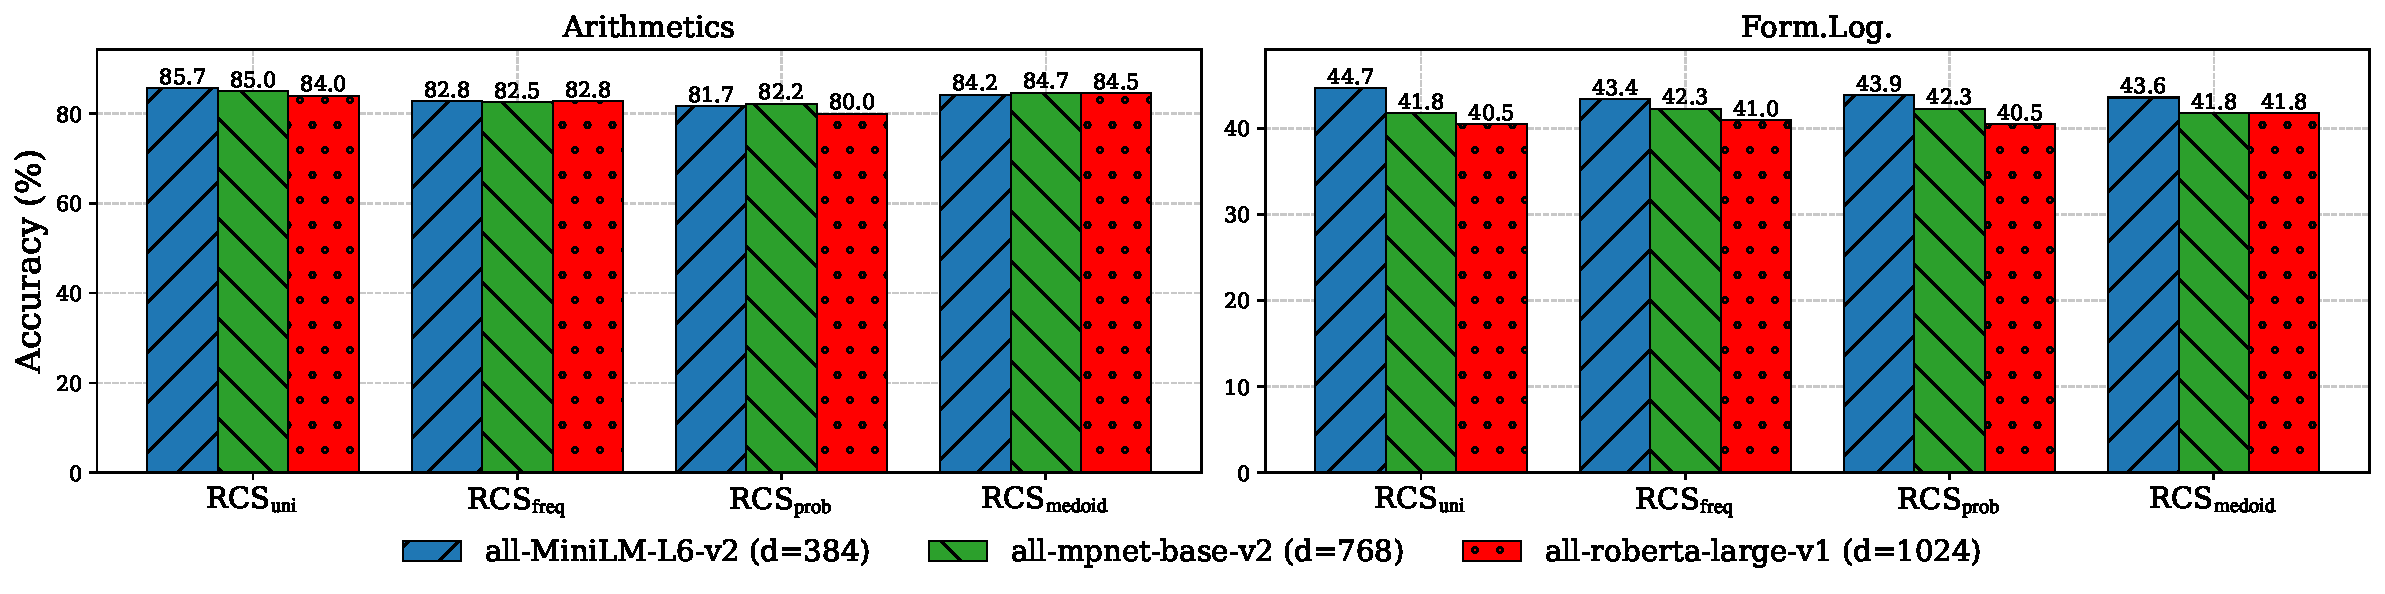
\includegraphics[width=\linewidth]{plots/abl_qwen2.5-3b_embedding_v3.pdf}
    \caption{
    Effect of the sentence embedding model on Arithmetics and Form.Log. using Qwen2.5-3B.
    }
    \label{fig:embed_qwen2.5-3b}
\end{figure*}

\begin{figure*}[ht]
    \centering
    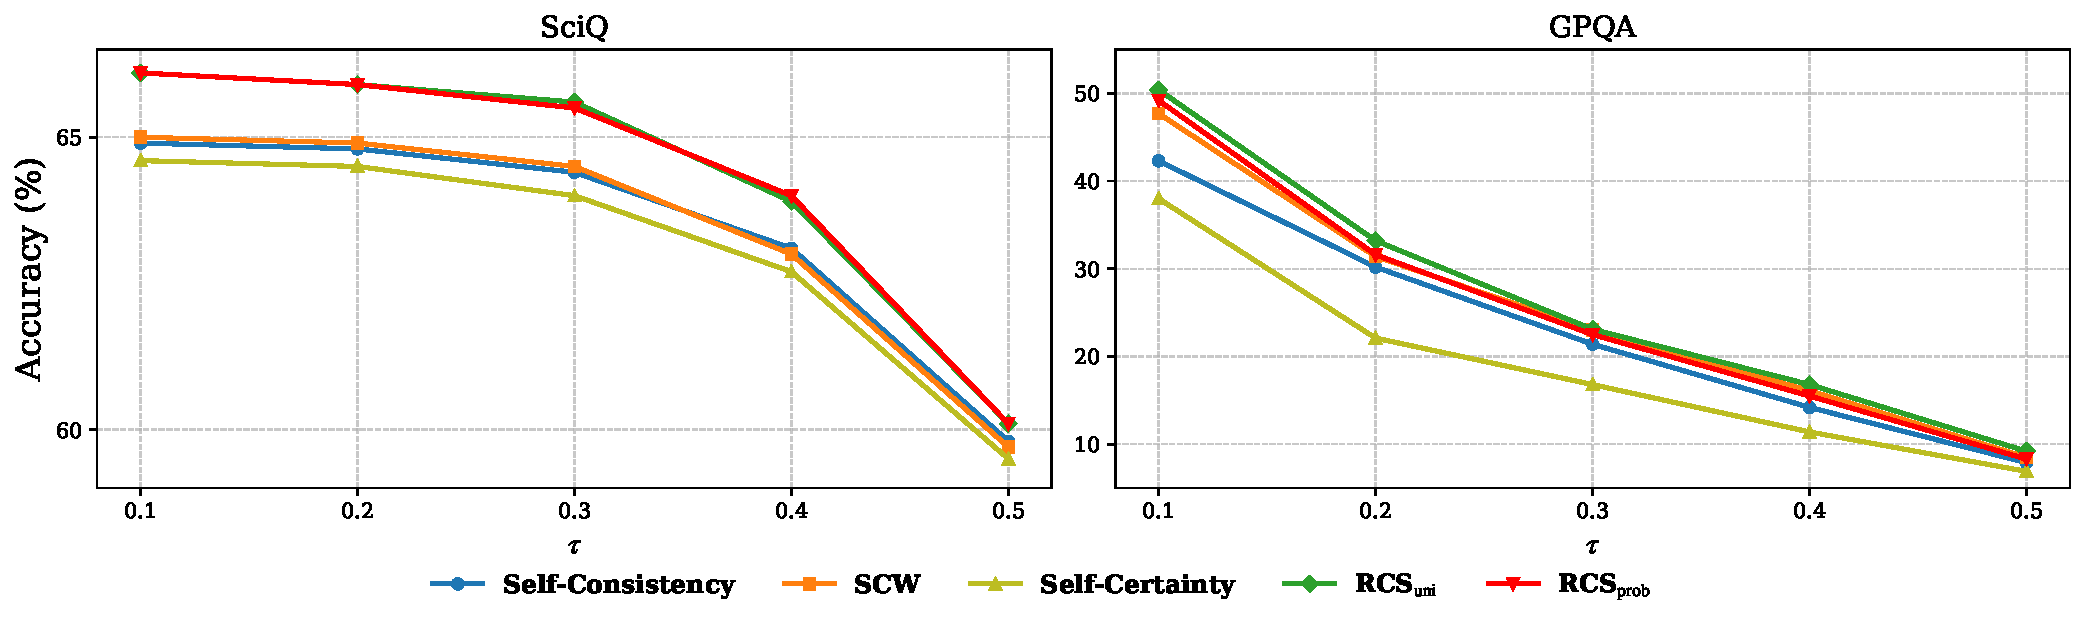
\includegraphics[width=\linewidth]{plots/abl_qwen2.5-3b_threshold_v6.pdf}
    \caption{
    Performance on SciQ and GPQA when varying correctness threshold ($\tau$) using Llama3.2-3B.
    }
    \label{fig:threshold_llama3.2-3b}
\end{figure*}

% -----------
\begin{figure*}[t]
    \centering
    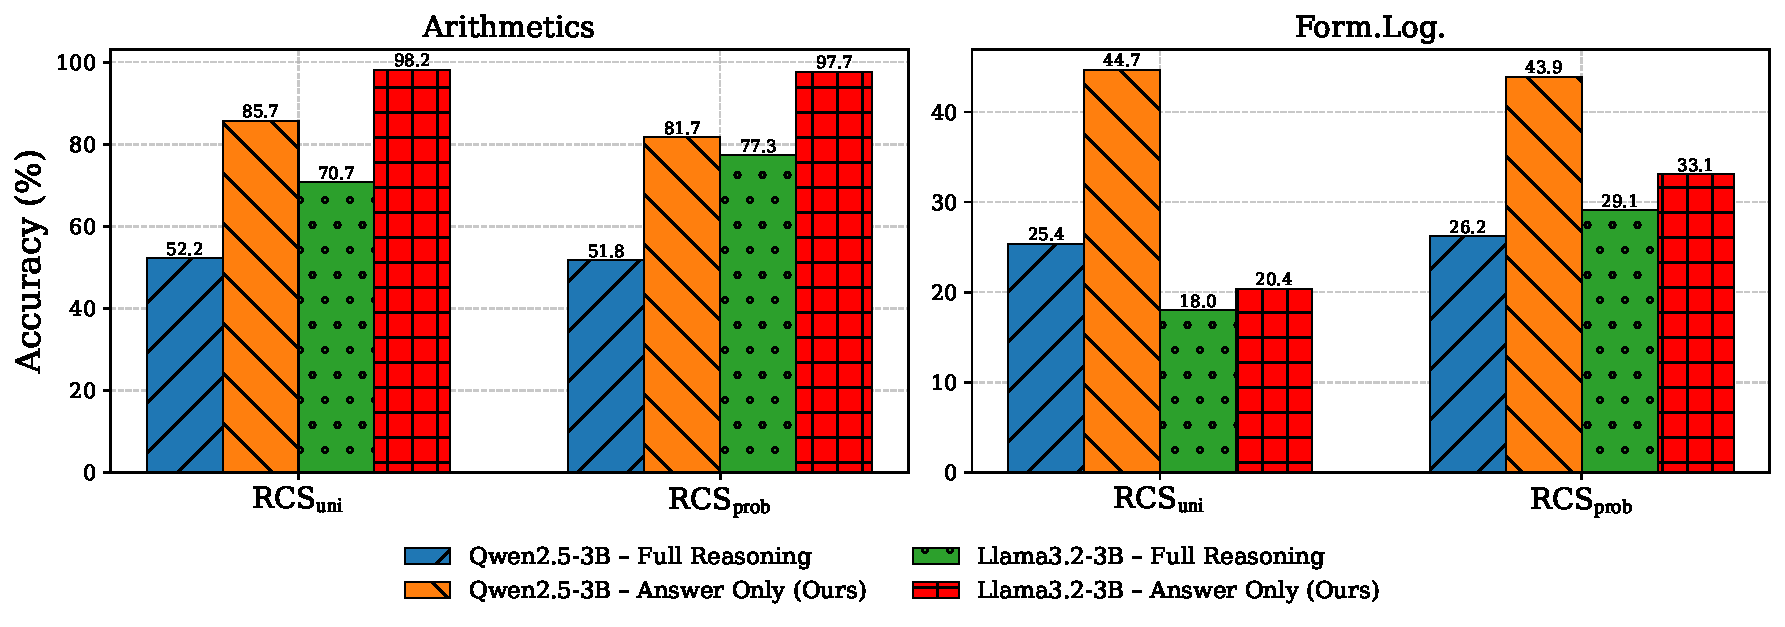
\includegraphics[width=\linewidth]{plots/abl_qwen2.5-3b_llama3.2-3b_full_vs_answer_v4.pdf}
    \caption{
    Effect of reasoning paths on Arithmetics and Form.Log. using Qwen2.5-3B and Llama3.2-3B. 
    % Similar results for Llama3.2-3B are provided in Appendix Figure~\ref{fig:full_llama3.2-3b}.
    }
    \label{fig:full}
\end{figure*}

% \begin{figure*}[t]
%     \centering
%     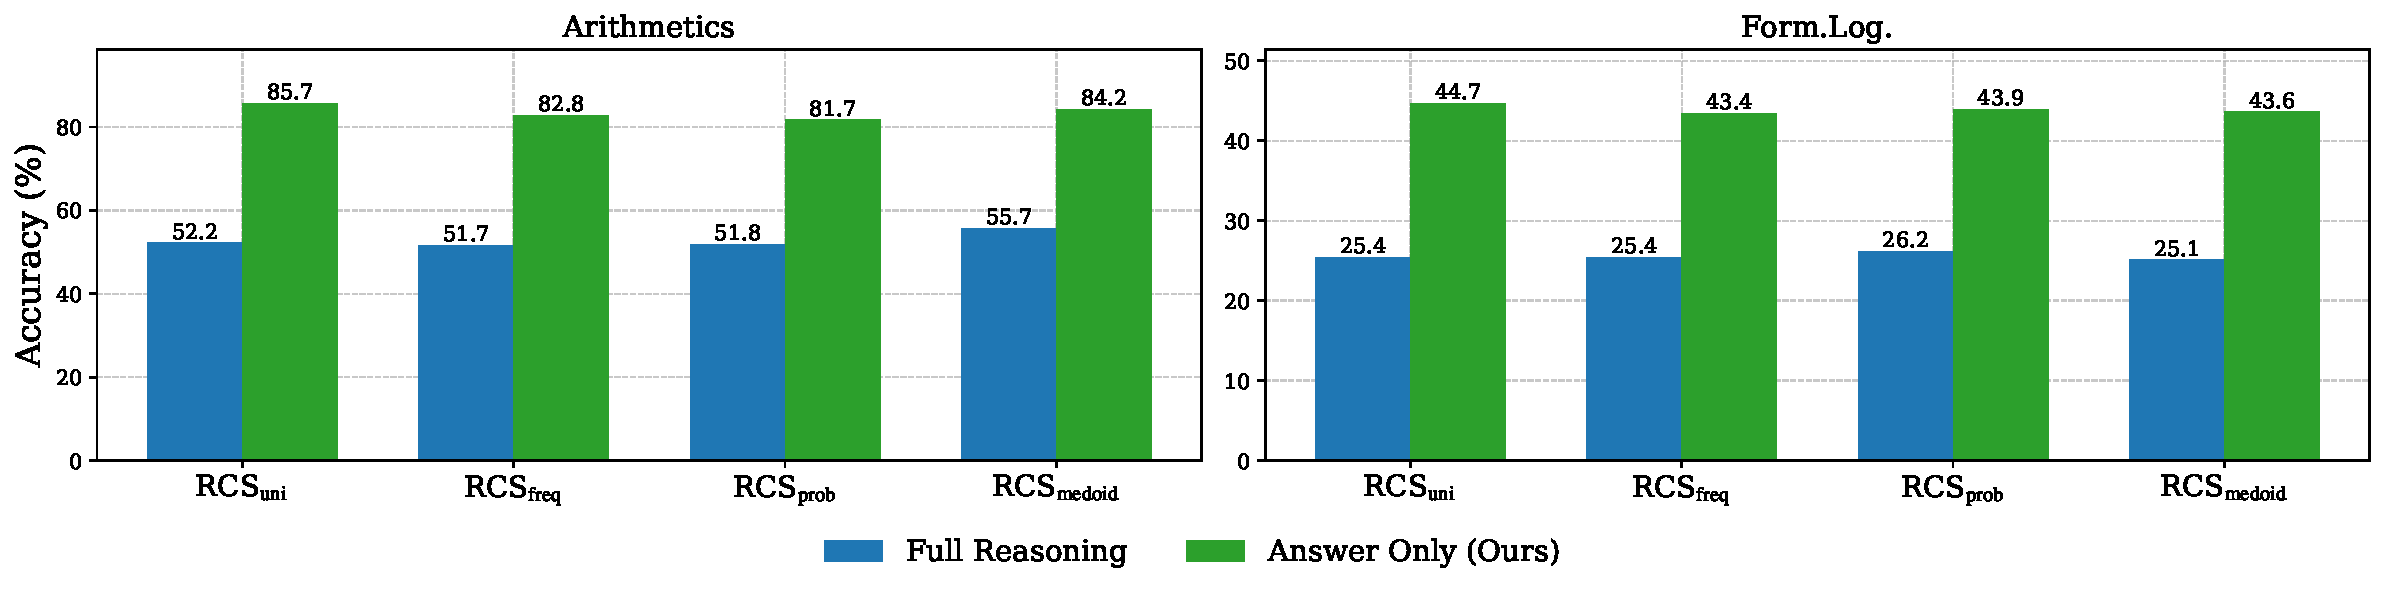
\includegraphics[width=\linewidth]{plots/abl_qwen2.5-3b_full_vs_answer_v3.pdf}
%     \caption{
%     Effect of reasoning paths on Arithmetics and Form.Log. using Qwen2.5-3B. 
%     % Similar results for Llama3.2-3B are provided in Appendix Figure~\ref{fig:full_llama3.2-3b}.
%     }
%     \label{fig:full_qwen2.5-3b}
% \end{figure*}

% \begin{figure*}[ht]
%     \centering
%     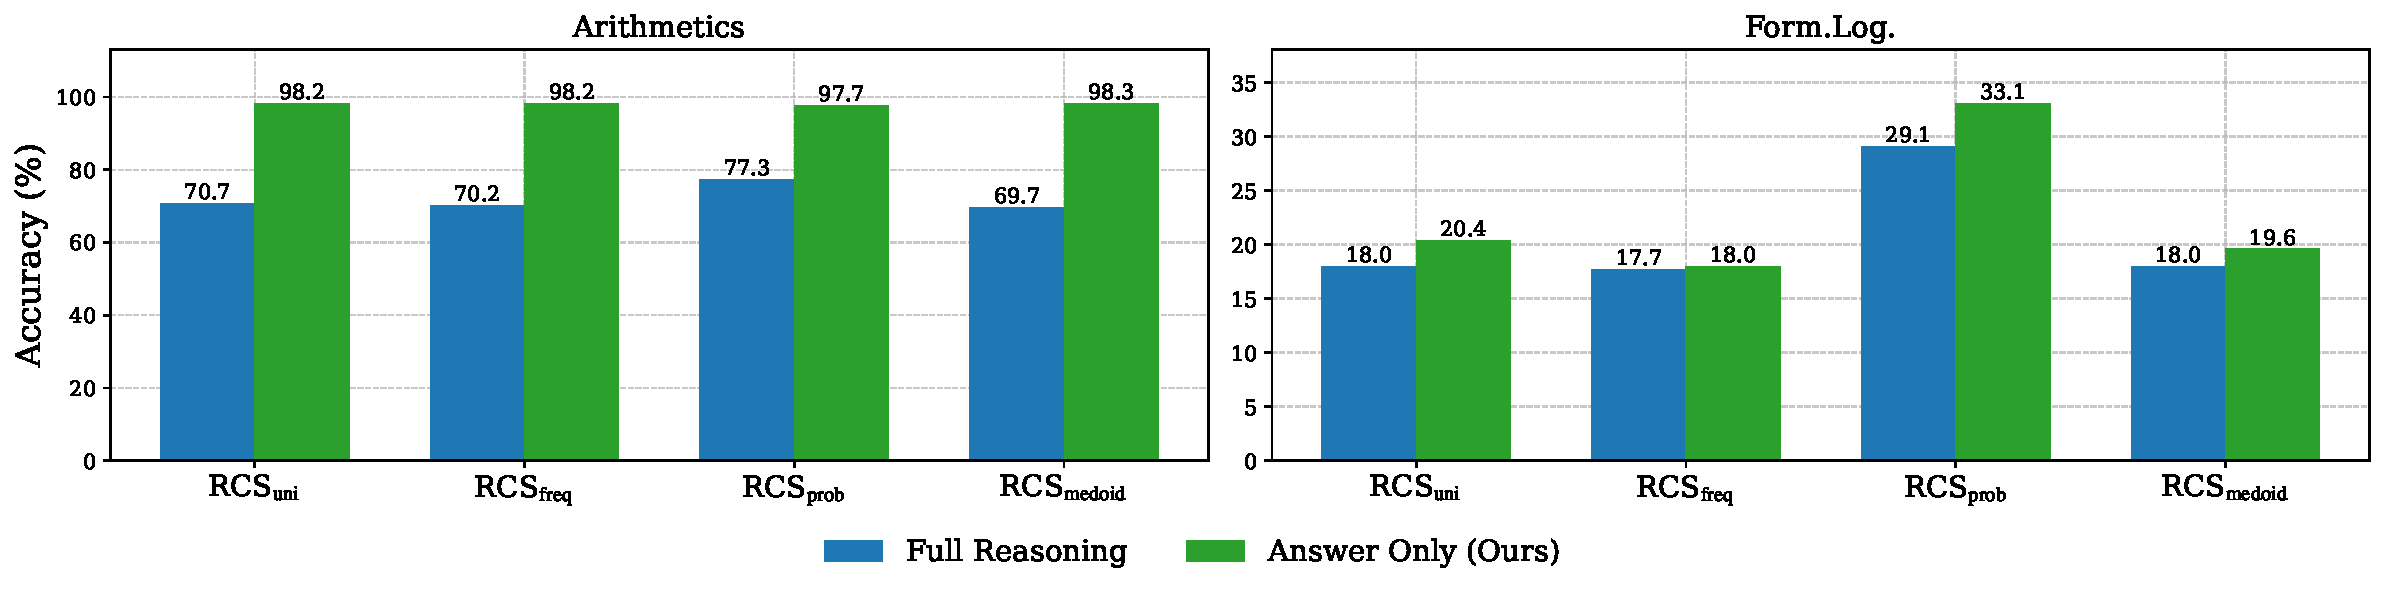
\includegraphics[width=\linewidth]{plots/abl_llama3.2-3b_full_vs_answer_v3.pdf}
%     \caption{
%     Effect of reasoning paths on Arithmetics and Form.Log. using Llama3.2-3B.}
%     \label{fig:full_llama3.2-3b}
% \end{figure*}




% ======================SCALABILITY =====================================
\subsection{Extended Results: Number Of Samples}\label{app:sample-details}

Tables~\ref{tab:ranking_n5},~\ref{tab:ranking_n20}, and~\ref{tab:ranking_n40} report performance over different number of sampling responses. 

\begin{table}[t]
  \centering
  \caption{Best-of-$N$ selection accuracy across settings ($N{=}5$).}
  \label{tab:ranking_n5}
  \resizebox{\columnwidth}{!}{
  \begin{tabular}{ll|ccccc}
    \toprule
    \textbf{Model} & \textbf{Method}
    & \textbf{SciQ} & \textbf{GPQA} 
    & \textbf{Arithmetics} & \textbf{GSM8K} & \textbf{Form.Log.} 
    \\
    \midrule
    \multirow{11}{*}{Qwen2.5-3B}
    & NLL & 61.7$\pm$1.2 &	17.6$\pm$3.1	& 49.2$\pm$12.4	& 45.2$\pm$4.7 &	28.0$\pm$3.2\\
    & ANLL & 61.6$\pm$1.1	& 17.1$\pm$4.1	& 48.7$\pm$11.4	& 46.0$\pm$4.8	& 27.5$\pm$3.3\\
    & SC  & 63.8$\pm$0.5	& 18.1$\pm$2.7	& 78.7$\pm$7.2	& 65.0$\pm$0.5	& 39.4$\pm$1.8\\
    & CE    & 63.6$\pm$0.3	& 15.7$\pm$1.7	& 78.5$\pm$7.4	& 66.8$\pm$5.0	& 42.4$\pm$0.2\\
    & ModeX    & 61.2$\pm$1.2	& 18.0$\pm$2.4	& 46.0$\pm$3.0	& 32.0$\pm$0.5	& 24.9$\pm$0.9\\
    & SCW & 64.0$\pm$0.2 & 24.0$\pm$2.6 & 72.2$\pm$2.5 & 55.8$\pm$2.2 & 36.8$\pm$1.2\\
    & RCS$_\text{medoid}$  &64.0$\pm$0.4	& 24.7$\pm$2.2	& 77.7$\pm$2.8	& 66.7$\pm$2.9	& 40.7$\pm$0.5\\
    & RCS$_\text{uni}$& 63.8$\pm$0.1	& 24.2$\pm$2.9	& 77.0$\pm$2.8	& 66.5$\pm$4.0	& 40.7$\pm$0.5 \\
    &  RCS$_\text{freq}$&64.0$\pm$0.2	& 24.0$\pm$2.6	& 77.5$\pm$3.1	& 66.3$\pm$3.8	& 41.0$\pm$0.5\\
    & RCS$_\text{cosine}$ & 63.9$\pm$0.2 & 24.9$\pm$2.4 & 72.8$\pm$2.5 & 55.5$\pm$2.4 & 36.5$\pm$1.4\\
    &  RCS$_\text{prob}$  &64.0$\pm$0.5	& 21.6$\pm$2.0	& 75.7$\pm$5.3	& 63.1$\pm$4.4	& 41.3$\pm$0.0\\
    \midrule
    
    \multirow{11}{*}{Qwen2.5-7B}
    & NLL & 67.6$\pm$1.5	& 17.1$\pm$1.4	& 63.3$\pm$10.9	& 51.4$\pm$3.4	& 36.0$\pm$2.3\\
    & ANLL & 67.5$\pm$1.1	& 16.9$\pm$1.2	& 63.5$\pm$11.0	& 51.4$\pm$3.4	& 35.4$\pm$2.0\\
    & SC  & 69.2$\pm$0.5	& 22.3$\pm$3.2	& 83.3$\pm$13.7	& 72.4$\pm$3.1	& 47.4$\pm$4.4\\
    & CE    & 69.4$\pm$0.1	& 19.9$\pm$1.1	& 84.0$\pm$16.0	& 74.3$\pm$2.6	& 47.8$\pm$3.6\\
    & ModeX & 69.0$\pm$0.7 & 22.1$\pm$3.0 & 54.2$\pm$3.2 & 40.6$\pm$2.7 & 34.1$\pm$6.3\\
    & SCW & 68.9$\pm$0.4 & 26.9$\pm$0.9 & 74.8$\pm$4.6 & 58.2$\pm$4.4 & 45.0$\pm$4.0\\
    & RCS$_\text{medoid}$  &69.0$\pm$0.4	& 27.3$\pm$0.8	&84.3$\pm$12.0	&74.3$\pm$1.8	&47.6$\pm$3.6\\
    & RCS$_\text{uni}$&68.9$\pm$0.4	&27.6$\pm$1.3	&84.2$\pm$11.8	&75.0$\pm$1.3	&47.6$\pm$3.6\\
    &  RCS$_\text{freq}$&69.0$\pm$0.4	&26.9$\pm$0.9	&84.3$\pm$12.0	&75.1$\pm$1.0	&47.6$\pm$3.6\\
    & RCS$_\text{cosine}$ & 69.0$\pm$0.4 & 27.5$\pm$1.0 & 74.8$\pm$6.0 & 60.1$\pm$2.4 & 45.2$\pm$4.4\\
    &  RCS$_\text{prob}$  &69.3$\pm$0.4	&25.2$\pm$1.5	&83.0$\pm$11.8	&70.9$\pm$2.0	&47.9$\pm$3.3\\
    \midrule

    \multirow{11}{*}{Llama3.2-3B}
    & NLL & 54.0$\pm$1.3	&19.2$\pm$0.9	&82.7$\pm$4.2	&73.4$\pm$3.8	&31.0$\pm$2.9\\
    & ANLL & 53.7$\pm$0.6	&18.5$\pm$2.0	&86.7$\pm$3.3	&76.1$\pm$1.8	&31.5$\pm$2.0\\
    & SC  & 58.6$\pm$0.8	&16.1$\pm$2.4	&93.3$\pm$2.1	&79.2$\pm$3.6	&31.5$\pm$1.7\\
    & CE    & 57.6$\pm$1.4	&19.2$\pm$3.2	&93.0$\pm$1.8	&80.3$\pm$4.1	&33.7$\pm$2.4\\
    & ModeX    & 53.4$\pm$1.1&	12.8$\pm$3.2	&68.8$\pm$1.0	&61.3$\pm$2.6	&19.1$\pm$3.5\\
    & SCW & 59.4$\pm$1.2 & 22.3$\pm$2.6 & 90.5$\pm$2.1 & 74.3$\pm$0.3 & 22.0$\pm$5.4\\
    & RCS$_\text{medoid}$  &59.4$\pm$1.2	&22.5$\pm$2.9	&94.0$\pm$0.5	&80.2$\pm$2.0	&30.9$\pm$4.8\\
    & RCS$_\text{uni}$& 59.3$\pm$1.5	&22.3$\pm$2.6	&93.3$\pm$0.6	&80.4$\pm$2.1	&30.9$\pm$4.8\\
    &  RCS$_\text{freq}$&59.4$\pm$1.2	&22.3$\pm$2.6	&93.8$\pm$0.8	&80.4$\pm$2.1	&30.9$\pm$4.8\\
    & RCS$_\text{cosine}$ & 59.3$\pm$1.4 & 22.5$\pm$2.9 & 92.8$\pm$1.1 & 76.3$\pm$1.6 & 20.9$\pm$4.4\\
    &  RCS$_\text{prob}$  &58.9$\pm$1.4	&21.2$\pm$3.6	&93.5$\pm$1.5	&80.0$\pm$1.9	&32.8$\pm$2.4\\
    \midrule

    \multirow{11}{*}{Llama3.1-8B}
    & NLL & 61.2$\pm$0.6	&21.1$\pm$1.1&	73.3$\pm$2.5&	72.8$\pm$3.3&	38.9$\pm$1.4\\
    & ANLL & 60.8$\pm$0.5	&20.7$\pm$1.4	&73.2$\pm$3.3	&73.3$\pm$3.1&	38.4$\pm$1.8\\
    & SC  & 66.0$\pm$1.8	&19.2$\pm$1.9&	82.2$\pm$7.2&	82.6$\pm$3.8	&43.1$\pm$3.9\\
    & CE    & 65.6$\pm$0.4	&19.7$\pm$3.2	&82.1$\pm$8.4	&82.4$\pm$3.1	&42.4$\pm$3.0\\
    & ModeX    & 62.1$\pm$0.9	&20.5$\pm$2.1	&50.2$\pm$0.8	&53.5$\pm$3.8	&25.1$\pm$0.5\\
    & SCW & 67.1$\pm$0.7 & 26.8$\pm$1.3 & 79.0$\pm$0.5 & 69.5$\pm$1.3 & 34.7$\pm$0.9\\
    & RCS$_\text{medoid}$  &67.0$\pm$0.8	&27.3$\pm$1.3	&86.0$\pm$4.0	&83.2$\pm$5.2	&41.8$\pm$3.2\\
    & RCS$_\text{uni}$& 67.0$\pm$0.6	&26.9$\pm$2.1	&85.5$\pm$3.0	&83.2$\pm$5.6	&42.3$\pm$3.6\\
    &  RCS$_\text{freq}$&67.1$\pm$0.7	&26.8$\pm$1.3	&85.7$\pm$3.6	&83.2$\pm$5.6	&42.3$\pm$3.6\\
    & RCS$_\text{cosine}$ & 66.9$\pm$0.6 & 27.1$\pm$2.1 & 81.3$\pm$0.8 & 70.9$\pm$2.4 & 36.8$\pm$2.6\\
    &  RCS$_\text{prob}$  &66.7$\pm$0.8	&26.4$\pm$2.7	&77.3$\pm$3.6	&76.0$\pm$3.1	&39.2$\pm$4.1\\
    \midrule

    \multirow{11}{*}{Gemma2-9B}
    & NLL & 69.2$\pm$0.4	&27.1$\pm$1.1	&94.5$\pm$1.0	&87.3$\pm$0.9	&54.5$\pm$4.4\\
    & ANLL & 66.2$\pm$0.9	&21.1$\pm$1.1	&95.8$\pm$1.0	&87.8$\pm$1.3	&54.8$\pm$2.1\\
    & SC  & 72.8$\pm$0.6	&17.3$\pm$2.3	&97.0$\pm$0.9	&88.8$\pm$1.8	&55.6$\pm$5.0\\
    & CE    & 73.2$\pm$0.4	&17.8$\pm$3.5	&97.0$\pm$0.9&	89.8$\pm$2.1	&55.5$\pm$5.2\\
    & ModeX    & 71.5$\pm$0.6	&20.7$\pm$0.5	&92.5$\pm$1.0	&64.0$\pm$2.3	&52.1$\pm$6.5\\
    & SCW & 73.9$\pm$0.6 & 24.9$\pm$2.3 & 96.7$\pm$0.8 & 72.1$\pm$0.9 & 54.0$\pm$2.9\\

    & RCS$_\text{medoid}$  &73.7$\pm$0.7&	24.2$\pm$2.0&	96.8$\pm$0.6	&89.0$\pm$2.1&	55.3$\pm$4.8\\
    & RCS$_\text{uni}$& 73.8$\pm$0.4	&25.9$\pm$2.1	&96.8$\pm$0.6	&88.7$\pm$1.6	&55.8$\pm$4.8\\
    &  RCS$_\text{freq}$&74.0$\pm$0.6	&24.9$\pm$2.3	&96.8$\pm$0.6	&88.7$\pm$1.6	&55.6$\pm$4.4\\
    & RCS$_\text{cosine}$ & 73.8$\pm$0.5 & 25.7$\pm$2.2 & 96.8$\pm$0.6 & 72.8$\pm$1.1 & 54.0$\pm$4.2\\
    &  RCS$_\text{prob}$  &73.2$\pm$0.3	&24.2$\pm$1.3	&96.8$\pm$0.6&	88.8$\pm$1.5&	55.3$\pm$3.6\\
    
    \bottomrule
  \end{tabular}}
\end{table}

%% ===============N=20================
\begin{table}[t]
  \centering
  \caption{Best-of-$N$ selection accuracy across settings ($N{=}20$).}
  \label{tab:ranking_n20}
  \resizebox{\columnwidth}{!}{
  \begin{tabular}{ll|ccccc}
    \toprule
    \textbf{Model} & \textbf{Method}
    & \textbf{SciQ} & \textbf{GPQA} 
    & \textbf{Arithmetics} & \textbf{GSM8K} & \textbf{Form.Log.} 
    \\
    \midrule
    \multirow{11}{*}{Qwen2.5-3B}
    & NLL & 59.0$\pm$0.4	&16.4$\pm$2.3	&48.2$\pm$11.9	&40.6$\pm$0.5	&26.5$\pm$2.6\\
    & ANLL & 58.4$\pm$0.4	&16.2$\pm$2.6	&47.8$\pm$12.5	&40.8$\pm$1.1	&26.5$\pm$2.6\\
    & SC  & 64.9$\pm$0.6	&20.0$\pm$0.3	&95.3$\pm$5.1	&88.3$\pm$0.9	&48.1$\pm$3.6\\
    & CE    & 64.2$\pm$0.9	&18.3$\pm$1.3	&95.3$\pm$5.9	&88.8$\pm$0.9	&47.1$\pm$2.4\\
    & ModeX    & 62.2$\pm$0.8	&21.9$\pm$1.7	&51.7$\pm$3.4	&37.9$\pm$2.1	&23.3$\pm$1.8\\
    & SCW & 64.9$\pm$0.6 & 24.4$\pm$2.7 & 92.5$\pm$0.7 & 67.0$\pm$1.3 & 42.1$\pm$2.9\\

    & RCS$_\text{medoid}$  &65.0$\pm$0.7	&26.1$\pm$2.7	&96.5$\pm$3.5	&88.5$\pm$0.6	&47.4$\pm$4.1\\
    &RCS$_\text{uni}$& 65.5$\pm$1.0	&24.9$\pm$2.7	&96.7$\pm$2.4	&87.1$\pm$1.6	&48.1$\pm$4.4\\
    &  RCS$_\text{freq}$&64.7$\pm$0.5	&23.8$\pm$2.9&	96.3$\pm$3.3&	88.0$\pm$0.8	&47.6$\pm$5.0\\
    & RCS$_\text{cosine}$ & 65.3$\pm$0.9 & 25.2$\pm$2.9 & 94.2$\pm$1.1 & 70.4$\pm$1.8 & 42.3$\pm$3.9\\
    &  RCS$_\text{prob}$  &65.3$\pm$0.7	&24.9$\pm$2.4	&95.2$\pm$3.3	&86.6$\pm$1.1	&46.6$\pm$4.1\\
    \midrule
    
    \multirow{11}{*}{Qwen2.5-7B}
    & NLL & 66.5$\pm$0.8	&18.1$\pm$1.9	&63.3$\pm$11.2	&55.8$\pm$2.0	&30.7$\pm$4.8\\
    & ANLL & 66.5$\pm$1.0&	18.1$\pm$1.8	&63.5$\pm$12.2	&55.7$\pm$1.8	&31.2$\pm$4.4\\
    & SC  & 70.0$\pm$0.2	&26.3$\pm$0.6	&93.3$\pm$9.8	&93.1$\pm$1.3&	51.8$\pm$2.3\\
    & CE    & 69.9$\pm$0.2	&25.2$\pm$0.3	&93.7$\pm$9.7	&92.6$\pm$0.8&	52.9$\pm$2.6\\
    & ModeX & 68.5$\pm$1.2 & 24.0$\pm$2.6 & 59.5$\pm$0.0 & 37.9$\pm$1.5 & 31.2$\pm$3.6\\
    & SCW & 70.0$\pm$0.3 & 27.6$\pm$2.0 & 80.8$\pm$0.4 & 67.0$\pm$1.3 & 48.7$\pm$1.8\\
    & RCS$_\text{medoid}$  &69.7$\pm$0.3&	28.0$\pm$1.8	&95.0$\pm$6.9&	92.2$\pm$0.8	&52.6$\pm$1.7\\
    & RCS$_\text{uni}$&69.9$\pm$0.2	&28.7$\pm$2.2	&95.8$\pm$5.9	&91.7$\pm$1.1	&53.4$\pm$2.4\\
    &  RCS$_\text{freq}$&70.1$\pm$0.3	&28.0$\pm$1.6	&94.5$\pm$7.8	&92.7$\pm$1.1&	52.1$\pm$1.8\\
    & RCS$_\text{cosine}$ & 69.8$\pm$0.2 & 28.3$\pm$1.8 & 86.0$\pm$2.8 & 70.4$\pm$2.4 & 48.7$\pm$1.7\\
    &  RCS$_\text{prob}$  &70.0$\pm$0.3&	27.5$\pm$1.6&	95.3$\pm$6.8	&91.7$\pm$0.3	&53.4$\pm$3.2\\
    \midrule

    \multirow{11}{*}{Llama3.2-3B}
    & NLL & 53.0$\pm$0.5	&22.1$\pm$2.9	&90.2$\pm$0.8	&79.9$\pm$2.1	&39.7$\pm$0.0\\
    & ANLL & 52.8$\pm$0.9	&19.3$\pm$3.5	&91.7$\pm$0.3	&82.7$\pm$0.9	&39.9$\pm$5.3\\
    & SC  & 59.8$\pm$0.3	&15.7$\pm$0.8	&98.2$\pm$0.3	&89.3$\pm$1.3	&43.7$\pm$2.9\\
    & CE    & 60.0$\pm$0.6	&17.3$\pm$1.5	&98.2$\pm$0.3	&89.7$\pm$1.3	&45.0$\pm$3.0\\
    & ModeX    & 55.0$\pm$0.7	&16.9$\pm$3.2	&73.0$\pm$0.5	&61.8$\pm$5.7	&20.1$\pm$2.0\\
    & SCW & 60.3$\pm$0.4 & 25.0$\pm$2.6 & 97.5$\pm$nan & 84.1$\pm$1.3 & 24.6$\pm$2.4\\

    & RCS$_\text{medoid}$  &60.7$\pm$0.2&	26.1$\pm$3.4&	98.0$\pm$0.0&	89.5$\pm$1.3	&43.9$\pm$3.2\\
    & RCS$_\text{uni}$& 60.7$\pm$0.7	&26.8$\pm$2.9&	98.5$\pm$0.5	&89.5$\pm$1.6	&44.2$\pm$2.4\\
    &  RCS$_\text{freq}$&60.4$\pm$0.3	&25.7$\pm$2.9&	98.0$\pm$0.0	&89.3$\pm$1.3	&43.4$\pm$2.5\\
    & RCS$_\text{cosine}$ & 60.8$\pm$0.6 & 26.1$\pm$4.0 & 98.5$\pm$nan & 84.3$\pm$1.5 & 22.8$\pm$1.7\\
    &  RCS$_\text{prob}$  &60.7$\pm$0.5&	26.4$\pm$3.7	&98.0$\pm$0.0&	89.5$\pm$1.1&	42.1$\pm$2.4\\
    \midrule

    \multirow{11}{*}{Llama3.1-8B}
    & NLL & 61.0$\pm$1.5	&20.7$\pm$1.5&	81.2$\pm$4.3	&83.8$\pm$1.8&	48.9$\pm$1.8\\
    & ANLL & 61.1$\pm$1.9	&21.8$\pm$0.0	&79.8$\pm$3.9	&82.2$\pm$3.1&	44.4$\pm$2.1\\
    & SC  & 68.1$\pm$0.5	&18.9$\pm$0.4	&95.3$\pm$6.0	&91.9$\pm$1.3&	55.3$\pm$2.0\\
    & CE    & 68.2$\pm$0.6	&20.7$\pm$0.0	&94.8$\pm$7.2	&91.7$\pm$1.5&	54.0$\pm$2.1\\
    & ModeX    & 62.8$\pm$0.7	&22.3$\pm$0.5	&54.8$\pm$0.6	&49.9$\pm$3.6	&24.3$\pm$3.3\\
    & SCW & 68.3$\pm$0.1 & 32.4$\pm$0.4 & 92.3$\pm$0.8 & 84.3$\pm$1.3 & 39.7$\pm$3.5\\

    & RCS$_\text{medoid}$  &67.9$\pm$0.1	&35.8$\pm$0.7	&97.8$\pm$2.1	&92.2$\pm$1.8	&55.0$\pm$2.4\\
    & RCS$_\text{uni}$& 68.3$\pm$0.5	&36.0$\pm$1.1	&98.8$\pm$1.2	&91.4$\pm$1.8	&54.0$\pm$2.4\\
    &  RCS$_\text{freq}$&68.3$\pm$0.5	&33.7$\pm$0.7&	96.0$\pm$5.2&	92.2$\pm$1.8	&55.0$\pm$2.4\\
    & RCS$_\text{cosine}$ & 68.3$\pm$0.3 & 36.0$\pm$2.6 & 95.3$\pm$1.4 & 83.6$\pm$1.1 & 39.4$\pm$3.7\\
    &  RCS$_\text{prob}$  &68.1$\pm$0.3&	36.3$\pm$0.7	&97.2$\pm$1.2	&88.3$\pm$1.8	&52.9$\pm$3.0\\
    \midrule

    \multirow{11}{*}{Gemma2-9B}
    & NLL & 74.1$\pm$0.3	&27.1$\pm$1.1&	96.2$\pm$0.3&	89.3$\pm$0.9&	52.1$\pm$0.9\\
    & ANLL & 64.8$\pm$0.5&	23.0$\pm$1.1	&96.3$\pm$0.3	&89.8$\pm$0.9	&54.5$\pm$1.7\\
    & SC  & 74.1$\pm$0.8	&22.1$\pm$2.0&	97.2$\pm$0.3&	91.7$\pm$0.3	&54.0$\pm$0.8\\
    & CE    & 74.3$\pm$0.4&	21.8$\pm$0.5&	97.2$\pm$0.3&	91.7$\pm$0.8&	54.0$\pm$0.8\\
    & ModeX    & 73.0$\pm$0.4&22.1$\pm$1.6	&92.3$\pm$2.0&	64.8$\pm$1.1	&51.9$\pm$5.4\\
    & SCW & 74.1$\pm$0.5 & 28.8$\pm$2.0 & 97.0$\pm$0.5 & 75.8$\pm$0.3 & 51.3$\pm$0.5\\
    & RCS$_\text{medoid}$  &74.2$\pm$0.4	&28.7$\pm$1.7&	97.2$\pm$0.3&	91.7$\pm$0.3&	54.2$\pm$0.5\\
    & RCS$_\text{uni}$& 74.7$\pm$0.4	&29.9$\pm$1.3	&97.2$\pm$0.3	&91.7$\pm$0.3	&54.2$\pm$0.5\\
    &  RCS$_\text{freq}$&74.2$\pm$0.6&	29.4$\pm$2.1&	97.2$\pm$0.3	&91.9$\pm$0.0&	54.2$\pm$0.5\\
    & RCS$_\text{cosine}$ & 74.6$\pm$0.4 & 29.0$\pm$0.5 & 97.2$\pm$0.3 & 76.3$\pm$0.8 & 52.1$\pm$0.9\\
    &  RCS$_\text{prob}$  &74.6$\pm$0.6	&29.5$\pm$0.9	&97.2$\pm$0.3	&91.5$\pm$0.3	&54.2$\pm$0.9\\
    
    \bottomrule
  \end{tabular}}
\end{table}

%% ===============N=40================
\begin{table}[t]
  \centering
  \caption{Best-of-$N$ selection accuracy across settings ($N{=}40$).}
  \label{tab:ranking_n40}
  \resizebox{\columnwidth}{!}{
  \begin{tabular}{ll|ccccc}
    \toprule
    \textbf{Model} & \textbf{Method}
    & \textbf{SciQ} & \textbf{GPQA} 
    & \textbf{Arithmetics} & \textbf{GSM8K} & \textbf{Form.Log.} 
    \\
    \midrule
    \multirow{11}{*}{Qwen2.5-3B}
    & NLL & 56.3$\pm$0.8	&16.8$\pm$1.8	&45.3$\pm$13.0&	42.8$\pm$1.5&	25.9$\pm$3.8\\
    & ANLL & 56.1$\pm$0.9	&16.8$\pm$2.0	&44.8$\pm$13.3	&43.0$\pm$2.8&	25.1$\pm$3.8\\
    & SC  & 	65.2$\pm$0.4&	21.8$\pm$1.4	&97.3$\pm$2.9&	90.2$\pm$1.1&	49.5$\pm$1.2\\
    & CE    & 65.2$\pm$0.3	&20.4$\pm$2.7	&97.5$\pm$2.6	&90.4$\pm$0.5	&48.9$\pm$3.2\\
    & ModeX    & 63.0$\pm$1.0	&20.0$\pm$0.5&	49.8$\pm$3.2	&35.7$\pm$3.1&	25.7$\pm$6.7\\
    & SCW & 65.3$\pm$0.3 & 25.6$\pm$2.3 & 89.0$\pm$2.1 & 71.7$\pm$1.2 & 44.2$\pm$1.7\\
    & RCS$_\text{medoid}$  &65.5$\pm$0.5&	25.0$\pm$1.3	&98.2$\pm$1.5	&90.0$\pm$0.8	&47.9$\pm$1.2\\
    & RCS$_\text{uni}$& 65.7$\pm$0.7&	25.0$\pm$1.3	&98.5$\pm$1.3	&89.7$\pm$1.3	&48.4$\pm$0.8\\
    &  RCS$_\text{freq}$&65.3$\pm$0.5	&23.8$\pm$2.4&	97.7$\pm$2.4&	90.0$\pm$0.8	&47.6$\pm$2.1\\
    & RCS$_\text{cosine}$ & 65.7$\pm$0.7 & 25.7$\pm$0.6 & 97.2$\pm$1.1 & 76.1$\pm$2.2 & 44.7$\pm$1.2\\
    &  RCS$_\text{prob}$  &65.9$\pm$0.7&	24.4$\pm$1.0	&98.2$\pm$1.6&	89.3$\pm$1.3	&47.4$\pm$0.5\\
    \midrule
    
    \multirow{11}{*}{Qwen2.5-7B}
    & NLL & 66.0$\pm$0.4	&18.5$\pm$1.2&	63.0$\pm$10.1	&57.5$\pm$3.1&	30.7$\pm$4.4\\
    & ANLL & 65.9$\pm$0.6&	18.5$\pm$0.8	&62.8$\pm$9.3	&57.5$\pm$3.4&	30.4$\pm$3.2\\
    & SC  & 70.5$\pm$0.3	&26.1$\pm$1.6&	96.2$\pm$5.8	&94.4$\pm$0.5&	54.0$\pm$0.8\\
    & CE    & 70.4$\pm$0.6&	26.9$\pm$3.1	&96.3$\pm$5.5	&94.4$\pm$0.0&	53.7$\pm$1.2\\
    & ModeX & 69.6$\pm$0.3 & 25.0$\pm$1.7 & 53.2$\pm$1.8 & 38.6$\pm$1.8 & 31.2$\pm$2.6\\
    & SCW & 70.4$\pm$0.1 & 28.2$\pm$0.6 & 86.0$\pm$0.0 & 74.6$\pm$2.8 & 49.5$\pm$2.4\\
    & RCS$_\text{medoid}$  &70.0$\pm$0.1	&28.0$\pm$0.9	&97.2$\pm$4.0&	94.8$\pm$0.3&	53.2$\pm$2.1\\
    & RCS$_\text{uni}$&70.3$\pm$0.4	&29.0$\pm$0.9&	98.2$\pm$2.3&	94.6$\pm$0.3	&52.6$\pm$3.7\\
    &  RCS$_\text{freq}$&70.5$\pm$0.2	&27.5$\pm$0.5&	96.5$\pm$5.2	&94.6$\pm$0.3&	52.9$\pm$3.2\\
    & RCS$_\text{cosine}$ & 70.2$\pm$0.4 & 28.3$\pm$0.3 & 94.0$\pm$0.0 & 75.6$\pm$1.8 & 50.3$\pm$1.7\\
    &  RCS$_\text{prob}$  &70.4$\pm$0.4	&27.3$\pm$0.8&	97.5$\pm$3.5	&94.6$\pm$0.3&	52.4$\pm$3.5\\
    \midrule

    \multirow{11}{*}{Llama3.2-3B}
    & NLL & 53.4$\pm$0.3&	21.6$\pm$1.7	&93.5$\pm$2.6&	82.7$\pm$1.0&	36.2$\pm$4.0\\
    & ANLL & 52.8$\pm$0.6	&18.7$\pm$2.3&	93.3$\pm$2.5&	83.2$\pm$1.8&	41.8$\pm$5.7\\
    & SC  & 60.4$\pm$0.7	&17.6$\pm$0.9&	98.7$\pm$0.6&	91.2$\pm$0.8&	44.2$\pm$0.5\\
    & CE    & 60.2$\pm$0.4&	21.2$\pm$3.2	&98.8$\pm$0.3&	91.2$\pm$0.6&	43.1$\pm$0.9\\
    & ModeX    & 55.8$\pm$0.9	&19.0$\pm$2.9&	72.5$\pm$2.6	&57.0$\pm$4.1	&22.0$\pm$3.2\\
    & SCW & 60.6$\pm$0.9 & 24.7$\pm$2.4 & 98.8$\pm$0.4 & 86.6$\pm$1.1 & 22.2$\pm$4.2\\
    & RCS$_\text{medoid}$  &60.9$\pm$1.0	&29.4$\pm$1.6&	98.7$\pm$0.6&	91.2$\pm$0.6&	45.2$\pm$0.8\\
    & RCS$_\text{uni}$&	60.9$\pm$0.8	&29.4$\pm$2.0	&98.5$\pm$0.9	&90.4$\pm$0.5&	46.3$\pm$1.7\\
    &  RCS$_\text{freq}$&61.0$\pm$1.0&	26.9$\pm$1.9&	98.7$\pm$0.6&	90.9$\pm$0.5	&44.2$\pm$1.7\\
    & RCS$_\text{cosine}$ & 61.1$\pm$1.1 & 29.9$\pm$2.0 & 98.8$\pm$1.1 & 86.3$\pm$0.5 & 23.0$\pm$2.9\\
    &  RCS$_\text{prob}$  &61.0$\pm$0.6	&29.4$\pm$2.1	&98.3$\pm$0.3&	90.7$\pm$0.3&	44.7$\pm$2.8\\
    \midrule

    \multirow{11}{*}{Llama3.1-8B}
    & NLL & 61.8$\pm$0.9	&18.9$\pm$1.1&	83.7$\pm$1.2	&83.9$\pm$2.5&	46.8$\pm$2.1\\
    & ANLL & 61.3$\pm$0.8	&20.5$\pm$1.8&	84.0$\pm$1.7&	81.7$\pm$2.0&	43.4$\pm$4.0\\
    & SC  & 69.3$\pm$0.3	&19.7$\pm$0.7&	96.3$\pm$4.2&	93.2$\pm$0.8&	51.9$\pm$2.0\\
    & CE    & 68.5$\pm$0.4&	18.9$\pm$0.4&	96.5$\pm$4.3&	93.2$\pm$0.8&	51.1$\pm$1.7\\
    & ModeX    & 64.8$\pm$0.3&	19.3$\pm$2.7&	53.5$\pm$0.9&	51.4$\pm$1.6	&23.0$\pm$2.1\\
    & SCW & 69.2$\pm$0.4 & 25.6$\pm$1.1 & 98.8$\pm$0.8 & 85.8$\pm$0.5 & 37.6$\pm$1.2\\
    & RCS$_\text{medoid}$  &69.1$\pm$0.3	&31.6$\pm$0.7&	98.5$\pm$0.5&	92.4$\pm$0.5	&51.1$\pm$1.2\\
    & RCS$_\text{uni}$& 69.6$\pm$0.2	&31.4$\pm$0.4	&98.7$\pm$1.0&	92.2$\pm$0.3&	50.5$\pm$1.2\\
    &  RCS$_\text{freq}$&69.2$\pm$0.8&	28.2$\pm$1.8	&96.7$\pm$3.6&	93.1$\pm$0.6&	51.1$\pm$1.2\\
    & RCS$_\text{cosine}$ & 69.5$\pm$0.2 & 31.9$\pm$1.1 & 99.2$\pm$0.6 & 84.9$\pm$0.8 & 38.1$\pm$1.4\\
    &  RCS$_\text{prob}$  &69.6$\pm$0.4&	29.5$\pm$1.5&	98.5$\pm$0.9&91.9$\pm$1.3	&51.6$\pm$2.1\\
    \midrule

    \multirow{11}{*}{Gemma2-9B}
    & NLL & 74.2$\pm$0.1	&26.8$\pm$2.1&	96.0$\pm$0.5	&89.7$\pm$0.8&51.3$\pm$3.9\\
    & ANLL & 62.2$\pm$1.5	&20.7$\pm$1.6&	96.2$\pm$0.3&	89.5$\pm$1.8&	53.7$\pm$2.0\\
    & SC  & 	74.2$\pm$0.4	&22.5$\pm$0.8	&97.5$\pm$0.0	&91.7$\pm$0.8&	55.6$\pm$0.8\\
    & CE    & 74.2$\pm$0.3	&19.3$\pm$0.6&	97.5$\pm$0.0	&91.5$\pm$0.3	&55.3$\pm$1.2\\
    & ModeX    & 71.9$\pm$0.4 &	21.4$\pm$3.2&	93.5$\pm$0.5	&66.3$\pm$2.9	&54.0$\pm$2.4\\
    & SCW & 74.2$\pm$0.5 & 26.9$\pm$0.9 & 97.5$\pm$0.0 & 77.2$\pm$0.9 & 52.4$\pm$0.8\\
    & RCS$_\text{medoid}$  &74.4$\pm$0.4&	29.4$\pm$1.2	&97.5$\pm$0.0	&91.7$\pm$0.8&	55.0$\pm$0.9\\
    & RCS$_\text{uni}$& 74.4$\pm$0.8	&29.7$\pm$1.6&	97.5$\pm$0.0&	91.5$\pm$0.6	&54.8$\pm$0.8\\
    &  RCS$_\text{freq}$&74.2$\pm$0.4&	28.0$\pm$1.0	&97.5$\pm$0.0	&91.7$\pm$0.8	&55.3$\pm$1.2\\
    & RCS$_\text{cosine}$ & 74.3$\pm$0.6 & 29.9$\pm$0.8 & 97.5$\pm$0.0 & 76.7$\pm$0.9 & 52.6$\pm$0.5\\
    &  RCS$_\text{prob}$  &74.4$\pm$0.5&	29.7$\pm$0.8	&97.3$\pm$0.3&	91.2$\pm$0.8&	55.3$\pm$0.5\\
    
    \bottomrule
  \end{tabular}}
\end{table}


\clearpage
\input{checklist}

\end{document}
